\documentclass[11pt,a4paper]{article}
\usepackage[utf8]{inputenc}
\usepackage[T1]{fontenc}
\usepackage[brazilian]{babel}
\usepackage{amsmath,amssymb}
\usepackage{booktabs,longtable,array}
\usepackage{graphicx}
\usepackage[a4paper,margin=1.8cm]{geometry}
\usepackage[hidelinks]{hyperref}
\usepackage[font=small,labelfont=bf,skip=4pt]{caption}
\setlength{\emergencystretch}{3em}\setlength{\parindent}{1.2em}\setlength{\parskip}{3pt}
\title{Backbones para a Neural Fourier Head: relat\'orio do experimento de 21/11/2026}
\author{Gerado por \texttt{codigo/relatorio.py} a partir dos CSV de \texttt{resultados/}}
\date{}
\begin{document}
\maketitle

\section*{Como ler este relatório}
Este relatório foi gerado por código; nenhum número do texto foi digitado à mão (todos estão em \texttt{numeros.json}). Os casos de vitória da NFH foram \emph{procurados} (exemplificação): eles mostram onde a NFH iguala ou supera a camada densa, e não valem como regra geral. Todas as combinações testadas e todas as derrotas aparecem aqui. Nas tabelas, ``densa+E'' é a camada densa treinada por mais épocas, o controle das épocas extras que a NFH recebe no ajuste. Diferenças relativas são $\text{NFH}/\text{referência}-1$: valores negativos favorecem a NFH.

Arquivos lidos: \texttt{t1.csv} (1458 linhas válidas), \texttt{t2.csv} (528) e \texttt{confirmacao.csv} (172). Linhas de cabeçalho repetidas descartadas: 0, 0 e 0. Linhas duplicadas (mesma tarefa e variante) descartadas: 0, 0 e 0.

\section*{Resumo dos resultados}
Funil: 226 combinações na T1, 105 qualificadas pela validação, 12 na T2 (16 pares combinação e largura), 14 pares qualificados, 8 na confirmação, 6 com SUCESSO e 2 com FALHA.

Dos 6 SUCESSO, 4 são sintéticos (SINT-M/PatchTST (largura 1), SINT-M/iTransformer (largura 2), SINT-U48/DLinear (largura 1) e SINT-U48/Linear (largura 1)) e 2 são de dados reais (ETTh2-U/FreqMLP (largura 1) e ETTh2-U/iTransformer (largura 1)), de 1 série real: ETTh2-U. Todos usam fração de treino de 0,1 a 0,25 (nenhum usa o treino inteiro). Eles foram procurados entre as combinações da T1 e valem só para esse recorte: não mostram que a NFH iguala a densa em dados reais em geral nem em \emph{backbones} em geral.

As 2 FALHAS são: ETTh1-M/PatchTST (largura 1), tipo ``falha pelo MAE'' (RMSE \textminus{}3,99\% e MAE +0,65\% contra a densa+E); ETTh1-M/PatchTST (largura 2), tipo ``falha pelo MAE'' (RMSE \textminus{}2,82\% e MAE +2,05\% contra a densa+E).
 Em ETTh1-M/PatchTST (largura 1) e ETTh1-M/PatchTST (largura 2), todos os modelos (densa, densa+E, \texttt{proj\_K10} e NFH) ficam acima da ingênua do último valor no RMSE médio de teste.


Na T1, a NFH vence a densa+E no teste nas duas métricas (RMSE e MAE) em 97 de 226 combinações, e a mediana da diferença relativa de RMSE de teste da melhor variante é +0,00\% (zero na precisão mostrada) contra a densa+E. Em 45 combinações a NFH ganhou na validação e perdeu no teste.

\textbf{Explicabilidade na SINT-M da varredura (resultado negativo).} Aqui o $y$ passado entra na janela ($d=5$; na dissertação $d=4$, sem $y$). ``Acerto'' é a fração das janelas de teste em que a variável de maior atribuição nos Integrated Gradients é a condutora conhecida. 
Em SINT-\allowbreak{}M\_\allowbreak{}M\_\allowbreak{}PatchTST\_\allowbreak{}w1\_\allowbreak{}f0.\allowbreak{}1, o acerto com as 5 colunas é 0,00 para a tendência e 0,00 para o ciclo (participação do $y$ passado na atribuição: 99,97\% e 100,00\%); só com as 4 covariáveis, 0,58 e 0,02. 
Em SINT-\allowbreak{}M\_\allowbreak{}M\_\allowbreak{}iTransformer\_\allowbreak{}w2\_\allowbreak{}f0.\allowbreak{}25, o acerto com as 5 colunas é 0,00 para a tendência e 0,00 para o ciclo (participação do $y$ passado na atribuição: 99,99\% e 100,00\%); só com as 4 covariáveis, 0,46 e 0,02. 
A atribuição não recupera a verdade conhecida quando o alvo passado está na entrada. Isso limita a alegação de explicação conferida nesta varredura; o resultado positivo da dissertação é de outra configuração.

Na T2, 3 pares qualificaram, não foram à confirmação e tiveram RMSE ou MAE de teste pior que o da densa+E; eles estão na Seção~\ref{sec:naoganhou}.

\section{Protocolo em uma página}
O protocolo foi escrito em 21/11/2026, antes de qualquer execução (\texttt{INSTRUCOES.md}). A pergunta é em que \emph{backbones} e conjuntos a NFH, no lugar da camada densa final, tem RMSE \textbf{e} MAE de teste iguais ou menores que os da densa. Todos os modelos têm a forma \texttt{InstanceNorm(Backbone + cabeça)}, com janela $L=96$, horizonte $H=48$, $q=2$, divisão cronológica 70/15/15 e a mesma semente, o mesmo otimizador (Adam, taxa $10^{-3}$) e os mesmos dados para a densa e a NFH; a cabeça NFH tem os mesmos $H(p+1)$ parâmetros da densa.

\textbf{Seleção só na validação.} Em cada etapa, a combinação e a variante NFH candidata são escolhidas pelo RMSE de validação relativo à densa+E (e o MAE de validação relativo precisa ser menor ou igual a zero); \texttt{selecionar.py} nem carrega as colunas de teste. O teste só entra na confirmação e neste relatório.

\textbf{Controle densa+E.} A densa é treinada por mais 15 épocas com taxa $10^{-4}$, sem penalização, escolhendo a época de menor RMSE de validação. A NFH é comparada com ela e com a densa simples; a densa+E tem, por construção, RMSE de validação menor ou igual ao da densa.

\textbf{Etapas.} T1 (triagem: todos os \emph{backbones}, largura 1, semente 0), T2 (as combinações selecionadas, sementes 0, 1, 2, larguras 1 e 2) e confirmação no teste com \textbf{sementes novas} (10 a 14), com a densa, a densa+E, a projeção \texttt{proj\_K10} e a variante NFH escolhida.

\textbf{Critério de sucesso (\S{}6).} Média do RMSE de teste \emph{e} média do MAE de teste da NFH menores ou iguais às da densa \emph{e} às da densa+E, e RMSE de teste da NFH menor que o da densa+E em pelo menos 4 das 5 sementes. Só as combinações com SUCESSO são citadas como exemplos em que a NFH iguala ou supera a densa; as demais são derrotas ou falhas do critério (pelo MAE ou pelas vitórias).

\textbf{Mudanças registradas no \S{}10} (texto integral no Apêndice~\ref{ap:s10}):
\begin{itemize}\setlength{\itemsep}{0pt}
\item \textbf{21/11/2026}: versão inicial (coordenador).
\item \textbf{21/11/2026, 16h10} (coordenador): antes de qualquer execução de T1, com base no relatório do pesquisador (\texttt{pesquisa/\allowbreak{}relatorio\_\allowbreak{}backbones.\allowbreak{}md}) e na revisão do código (\texttt{.\allowbreak{}kiro/\allowbreak{}specs/\allowbreak{}rodada-\allowbreak{}20261121/\allowbreak{}logs/\allowbreak{}revisao\_\allowbreak{}codigo.\allowbreak{}md}): 1. \textbf{Backbone acrescentado:} \texttt{FreqMLP} (rfft da janela, bins k = 1..12 em parte real e imaginária, duas camadas com GELU, p = 64$\cdot$largura), como...
\item \textbf{21/11/2026, 17h20} (coordenador): \textbf{Exemplo passo a passo (\S{}9), pré-registro.} Para que as contas caibam à mão, o exemplo não usa os \emph{backbones} grandes da T1: usa a série de livro de \texttt{teste\_\allowbreak{}exemplificacao\_\allowbreak{}nfh/\allowbreak{}exemplo\_\allowbreak{}livro/\allowbreak{}gerar.\allowbreak{}py} (H = 8, q = 1, K = 2, L = 16, d = 4, alvo y\_t = x1\_\{t$-$8\} + x2\_\{t$-$8\} + ruído, y fora da entrada, oráculo linear conhecido), com ru...
\item \textbf{21/11/2026, 18h15} (coordenador): \textbf{por tempo de máquina}, antes de rodar qualquer seleção sobre a T1 e sem ler colunas de teste: as tarefas da T1 duram de 12 a 92 min (TCN em CPU), e a ETA da T1 passou a \textasciitilde{}9 h. Para que T2 e confirmação terminem na manhã de 22/11: (1) um 9.º worker (GPU, \texttt{-\allowbreak{}-\allowbreak{}worker 8}) entrou na T1 às 18h10, com reivindicação dinâmica (não muda ...
\item \textbf{21/11/2026, 21h25} (coordenador): \textbf{depois da confirmação do exemplo passo a passo}, a pedido da auditoria externa (\texttt{.\allowbreak{}kiro/\allowbreak{}specs/\allowbreak{}rodada-\allowbreak{}20261121/\allowbreak{}avaliadores\_\allowbreak{}externos/\allowbreak{}20261121b\_\allowbreak{}exemplo\_\allowbreak{}auditor.\allowbreak{}md}, item 2): controle relatado da densa projetada em T $\oplus$ S, sem treino (\texttt{exemplo\_\allowbreak{}sintetico/\allowbreak{}projetar\_\allowbreak{}confirmacao.\allowbreak{}py}; ŷ $-$ QQᵀŷ nas sementes 10 a 19; confere que a densa re...
\item \textbf{22/11/2026, 18h28} (coordenador): \textbf{retomada depois do desligamento da máquina (21/11 21h33)}. Nada muda no protocolo: mesmas filas (\texttt{filas/\allowbreak{}t2.\allowbreak{}json}, md5 22ac3027..., gerada pela seleção automática de 21/11 21h14), mesmas regras de seleção e de confirmação, mesmo código de treino. Só muda a alocação: o controle das épocas (\texttt{experimento\_\allowbreak{}controle\_\allowbreak{}epocas/\allowbreak{}}) tem prio...
\item \textbf{22/11/2026, 23h07} (coordenador): \textbf{registro que faltava}, a pedido da auditoria externa (\texttt{.\allowbreak{}kiro/\allowbreak{}specs/\allowbreak{}rodada-\allowbreak{}20261121/\allowbreak{}avaliadores\_\allowbreak{}externos/\allowbreak{}20261122\_\allowbreak{}backbones\_\allowbreak{}auditor.\allowbreak{}md}, \S{}6 e \S{}9 item 6). Nada muda no protocolo nem em nenhum resultado. O exemplo passo a passo (\S{}9 e o registro de 21/11 17h20) \textbf{não usa} os hiperparâmetros do \S{}3. Valores de `exemplo\_sintetico/p...
\item \textbf{23/11/2026, 09h10} (coordenador): \textbf{depois de todos os resultados}, ao preparar o repositório público: o rótulo de licença do OPSD em \texttt{dados/\allowbreak{}baixar\_\allowbreak{}dados.\allowbreak{}py} (l. 212) e \texttt{dados/\allowbreak{}catalogo.\allowbreak{}json} dizia "CC BY 4.0", o que a página do pacote não sustenta (a licença dos dados não é declarada; ver \texttt{DATA.\allowbreak{}md} do repositório público, seção OPSD). O rótulo foi trocado por "...
\end{itemize}
\section{Contagens}
\textbf{T1.} A T1 testou 226 combinações (conjunto, modo, \emph{backbone}, fração) em 10 \emph{backbones} e 14 conjuntos (12 nomes de conjunto; ETTh1 e opsd\_de\_solar entram nos modos U e M, e cada modo conta como um conjunto, o que dá 14). Para cada combinação a melhor variante NFH foi escolhida só pelo RMSE de validação. Contra a densa+E, essa variante venceu em RMSE de validação em 129 combinações e, separadamente, em RMSE de teste em 112; venceu em RMSE \emph{e} MAE em 105 (validação) e 97 (teste). Em 45 combinações a NFH ganhou na validação e perdeu no teste (a escolha da melhor entre as variantes NFH da T1, 3 a 4 por combinação, favorece a NFH na validação, o que explica parte da diferença).
 Qualificaram pelo critério da validação 105 combinações e 12 foram para a T2 (\texttt{selecao\_T1.md}).
 A fila da T2 tem 48 tarefas de treino em 16 combinações com largura.


\textbf{T2.} A T2 deixou resultados completos (as sementes 0, 1, 2) em 16 pares (combinação, largura), de 12 combinações. A melhor variante (pela média do RMSE de validação relativo) venceu a densa+E no RMSE de validação em 16 pares e, separadamente, no RMSE de teste em 13 (em RMSE e MAE: 12). Qualificaram 14 pares (selecao\_T2.md)
 e 8 foram para a confirmação.


\textbf{Confirmação.} 8 combinações foram confirmadas com sementes novas: 6 com SUCESSO e 2 com FALHA (0 derrotas no RMSE médio, 2 falhas pelo MAE e 0 falhas pelas vitórias, definidas na Seção~\ref{sec:naoganhou})
.

\section{Triagem T1}
A Tabela~\ref{tab:t1_contagem_bb} dá as contagens por \emph{backbone} e a Tabela~\ref{tab:t1_contagem_cj} por conjunto e fração. As Tabelas~\ref{tab:t1_bb_val} e \ref{tab:t1_bb_test} resumem, por \emph{backbone}, a diferença relativa da melhor variante NFH (escolhida na validação) contra a densa+E e contra a densa, em RMSE e MAE: mediana e, entre colchetes, primeiro e terceiro quartis. As Tabelas~\ref{tab:t1_cj_val} e \ref{tab:t1_cj_test} fazem o mesmo por conjunto e fração.

\begin{table}[htbp]
\centering
\scriptsize
\setlength{\tabcolsep}{2pt}
\caption{T1: combina\c{c}\~oes testadas e vit\'orias da NFH sobre a densa+E, por backbone. ``Vence'' = RMSE (ou RMSE e MAE) menor que o da densa+E, da melhor variante NFH escolhida na valida\c{c}\~ao.}\label{tab:t1_contagem_bb}
\begin{tabular}{lrrrrrrr}
\toprule
Backbone & Comb. & \shortstack[l]{RMSE val} & \shortstack[l]{RMSE teste} & \shortstack[l]{RMSE+MAE val} & \shortstack[l]{RMSE+MAE teste} & Qualif. & \shortstack[l]{Foram T2} \\ \midrule
Conv1D+LSTM & 22 & 17 & 13 & 13 & 12 & 13 & 2 \\
DLinear & 22 & 10 & 12 & 7 & 12 & 7 & 1 \\
FreqMLP & 22 & 15 & 8 & 11 & 8 & 11 & 2 \\
LSTM & 22 & 14 & 11 & 12 & 8 & 12 & 0 \\
Linear & 22 & 8 & 9 & 6 & 9 & 6 & 1 \\
MLP & 22 & 10 & 11 & 8 & 8 & 8 & 0 \\
PatchTST & 24 & 18 & 15 & 17 & 13 & 17 & 3 \\
TCN & 22 & 4 & 9 & 4 & 8 & 4 & 0 \\
TSMixer & 24 & 15 & 14 & 12 & 10 & 12 & 0 \\
iTransformer & 24 & 18 & 10 & 15 & 9 & 15 & 3 \\
\bottomrule
\end{tabular}
\par\smallskip{\scriptsize Fonte: resultados/t1.csv e selecao\_T1.md.}
\end{table}


\begin{table}[htbp]
\centering
\scriptsize
\setlength{\tabcolsep}{2pt}
\caption{T1: combina\c{c}\~oes testadas e vit\'orias da NFH sobre a densa+E, por conjunto e fração. ``Vence'' = RMSE (ou RMSE e MAE) menor que o da densa+E, da melhor variante NFH escolhida na valida\c{c}\~ao.}\label{tab:t1_contagem_cj}
\begin{tabular}{lrrrrrrr}
\toprule
\shortstack[l]{Conjunto e\\ fração} & Comb. & \shortstack[l]{RMSE val} & \shortstack[l]{RMSE teste} & \shortstack[l]{RMSE+MAE val} & \shortstack[l]{RMSE+MAE teste} & Qualif. & \shortstack[l]{Foram T2} \\ \midrule
ETTh1-M f=0.25 & 3 & 3 & 1 & 3 & 1 & 3 & 2 \\
ETTh1-U f=0.25 & 10 & 9 & 4 & 8 & 4 & 8 & 0 \\
ETTh1-U f=1 & 10 & 9 & 5 & 8 & 3 & 8 & 0 \\
ETTh2-U f=0.25 & 10 & 9 & 8 & 7 & 7 & 7 & 2 \\
ETTh2-U f=1 & 10 & 6 & 7 & 6 & 7 & 6 & 0 \\
SINT-M-M f=0.1 & 10 & 8 & 8 & 7 & 8 & 7 & 1 \\
SINT-M-M f=0.25 & 10 & 8 & 8 & 8 & 8 & 8 & 1 \\
SINT-M-M f=1 & 10 & 7 & 7 & 7 & 7 & 7 & 1 \\
SINT-U48-U f=0.1 & 10 & 6 & 8 & 6 & 8 & 6 & 3 \\
SINT-U48-U f=0.25 & 10 & 9 & 5 & 8 & 5 & 8 & 0 \\
SINT-U48-U f=1 & 10 & 9 & 9 & 9 & 9 & 9 & 0 \\
air\_quality-U f=0.25 & 10 & 5 & 3 & 4 & 3 & 4 & 0 \\
air\_quality-U f=1 & 10 & 6 & 3 & 4 & 3 & 4 & 1 \\
bike\_sharing\_dc-U f=0.25 & 10 & 0 & 1 & 0 & 1 & 0 & 0 \\
bike\_sharing\_dc-U f=1 & 10 & 0 & 0 & 0 & 0 & 0 & 0 \\
electricity\_mt156-U f=0.25 & 10 & 3 & 5 & 1 & 1 & 1 & 0 \\
household\_power-U f=0.25 & 10 & 8 & 2 & 4 & 0 & 4 & 0 \\
jena\_climate-U f=0.25 & 10 & 4 & 8 & 2 & 6 & 2 & 0 \\
melbourne\_pedestrian\_southbank-U f=0.25 & 10 & 2 & 2 & 2 & 2 & 2 & 0 \\
melbourne\_pedestrian\_southbank-U f=1 & 10 & 2 & 1 & 2 & 1 & 2 & 0 \\
opsd\_de\_solar-M f=0.25 & 3 & 2 & 3 & 1 & 3 & 1 & 0 \\
opsd\_de\_solar-U f=0.25 & 10 & 3 & 4 & 0 & 3 & 0 & 0 \\
seoul\_bike-U f=0.25 & 10 & 5 & 7 & 2 & 5 & 2 & 0 \\
seoul\_bike-U f=1 & 10 & 6 & 3 & 6 & 2 & 6 & 1 \\
\bottomrule
\end{tabular}
\par\smallskip{\scriptsize Fonte: resultados/t1.csv e selecao\_T1.md.}
\end{table}


\begin{table}[htbp]
\centering
\scriptsize
\setlength{\tabcolsep}{2pt}
\caption{T1, valida\c{c}\~ao: diferen\c{c}a relativa da melhor variante NFH (escolhida na valida\c{c}\~ao), mediana [Q1; Q3], por backbone.}\label{tab:t1_bb_val}
\begin{tabular}{lrllll}
\toprule
Backbone & n & \shortstack[l]{RMSE vs\\ densa+E} & \shortstack[l]{MAE vs\\ densa+E} & \shortstack[l]{RMSE vs\\ densa} & \shortstack[l]{MAE vs\\ densa} \\ \midrule
Conv1D+LSTM & 22 & \textminus{}0,24\% [\textminus{}0,90; \textminus{}0,00] & \textminus{}0,13\% [\textminus{}0,88; +0,69] & \textminus{}1,00\% [\textminus{}2,07; \textminus{}0,00] & \textminus{}1,02\% [\textminus{}2,22; \textminus{}0,00] \\
DLinear & 22 & +0,00\% [\textminus{}0,08; +0,21] & +0,02\% [\textminus{}0,18; +0,17] & \textminus{}0,09\% [\textminus{}0,34; \textminus{}0,01] & \textminus{}0,11\% [\textminus{}1,14; \textminus{}0,00] \\
FreqMLP & 22 & \textminus{}0,06\% [\textminus{}0,91; +0,26] & \textminus{}0,06\% [\textminus{}0,64; +0,63] & \textminus{}0,51\% [\textminus{}1,20; \textminus{}0,03] & \textminus{}0,41\% [\textminus{}1,25; +0,00] \\
LSTM & 22 & \textminus{}0,07\% [\textminus{}0,34; +0,24] & \textminus{}0,00\% [\textminus{}0,29; +0,54] & \textminus{}0,28\% [\textminus{}1,47; \textminus{}0,00] & \textminus{}0,29\% [\textminus{}0,75; \textminus{}0,00] \\
Linear & 22 & +0,01\% [\textminus{}0,00; +0,21] & +0,07\% [\textminus{}0,00; +0,25] & \textminus{}0,04\% [\textminus{}0,28; \textminus{}0,00] & \textminus{}0,04\% [\textminus{}0,98; +0,00] \\
MLP & 22 & +0,06\% [\textminus{}0,06; +0,82] & +0,35\% [\textminus{}0,19; +1,28] & \textminus{}0,10\% [\textminus{}1,22; \textminus{}0,01] & \textminus{}0,33\% [\textminus{}1,60; \textminus{}0,00] \\
PatchTST & 24 & \textminus{}1,15\% [\textminus{}2,41; +0,03] & \textminus{}1,50\% [\textminus{}2,59; +0,12] & \textminus{}1,54\% [\textminus{}4,84; \textminus{}0,51] & \textminus{}2,25\% [\textminus{}4,90; \textminus{}0,31] \\
TCN & 22 & +0,06\% [+0,00; +0,48] & +0,03\% [\textminus{}0,00; +1,29] & \textminus{}0,00\% [\textminus{}0,29; +0,00] & +0,00\% [\textminus{}0,00; +0,00] \\
TSMixer & 24 & \textminus{}0,22\% [\textminus{}0,70; +0,17] & +0,00\% [\textminus{}0,50; +0,80] & \textminus{}0,36\% [\textminus{}1,12; \textminus{}0,00] & \textminus{}0,23\% [\textminus{}0,94; +0,00] \\
iTransformer & 24 & \textminus{}1,05\% [\textminus{}1,91; \textminus{}0,00] & \textminus{}1,02\% [\textminus{}1,79; +1,39] & \textminus{}1,57\% [\textminus{}2,91; \textminus{}0,50] & \textminus{}1,99\% [\textminus{}3,02; \textminus{}0,27] \\
\bottomrule
\end{tabular}
\par\smallskip{\scriptsize Fonte: resultados/t1.csv.}
\end{table}


\begin{table}[htbp]
\centering
\scriptsize
\setlength{\tabcolsep}{2pt}
\caption{T1, teste: diferen\c{c}a relativa da melhor variante NFH (escolhida na valida\c{c}\~ao), mediana [Q1; Q3], por backbone.}\label{tab:t1_bb_test}
\begin{tabular}{lrllll}
\toprule
Backbone & n & \shortstack[l]{RMSE vs\\ densa+E} & \shortstack[l]{MAE vs\\ densa+E} & \shortstack[l]{RMSE vs\\ densa} & \shortstack[l]{MAE vs\\ densa} \\ \midrule
Conv1D+LSTM & 22 & \textminus{}0,00\% [\textminus{}1,21; +0,33] & \textminus{}0,00\% [\textminus{}1,63; +1,33] & \textminus{}0,59\% [\textminus{}2,18; +0,00] & \textminus{}1,10\% [\textminus{}2,20; \textminus{}0,00] \\
DLinear & 22 & \textminus{}0,00\% [\textminus{}0,32; +0,05] & \textminus{}0,00\% [\textminus{}0,38; +0,11] & \textminus{}0,06\% [\textminus{}0,99; \textminus{}0,00] & \textminus{}0,08\% [\textminus{}1,40; \textminus{}0,00] \\
FreqMLP & 22 & +0,57\% [\textminus{}0,43; +1,11] & +0,20\% [\textminus{}0,51; +1,96] & +0,00\% [\textminus{}1,12; +0,52] & +0,00\% [\textminus{}1,34; +0,45] \\
LSTM & 22 & \textminus{}0,00\% [\textminus{}0,75; +0,88] & +0,54\% [\textminus{}0,22; +1,57] & \textminus{}0,33\% [\textminus{}0,80; +0,00] & \textminus{}0,00\% [\textminus{}1,01; +0,00] \\
Linear & 22 & +0,00\% [\textminus{}0,11; +0,13] & +0,00\% [\textminus{}0,10; +0,15] & \textminus{}0,05\% [\textminus{}0,99; \textminus{}0,00] & \textminus{}0,09\% [\textminus{}1,71; \textminus{}0,00] \\
MLP & 22 & \textminus{}0,02\% [\textminus{}0,48; +1,10] & +0,62\% [\textminus{}0,44; +1,63] & \textminus{}0,09\% [\textminus{}1,36; +0,00] & \textminus{}0,78\% [\textminus{}1,72; +0,00] \\
PatchTST & 24 & \textminus{}1,16\% [\textminus{}2,26; +0,58] & \textminus{}0,50\% [\textminus{}2,28; +0,77] & \textminus{}1,63\% [\textminus{}4,14; \textminus{}0,00] & \textminus{}2,00\% [\textminus{}4,41; \textminus{}0,00] \\
TCN & 22 & +0,11\% [\textminus{}0,00; +1,31] & +0,03\% [\textminus{}0,00; +2,43] & \textminus{}0,00\% [\textminus{}0,00; +0,00] & +0,00\% [\textminus{}0,00; +0,00] \\
TSMixer & 24 & \textminus{}0,00\% [\textminus{}0,86; +0,89] & +0,21\% [\textminus{}0,44; +1,77] & \textminus{}0,00\% [\textminus{}1,04; +0,00] & \textminus{}0,00\% [\textminus{}1,24; +0,06] \\
iTransformer & 24 & +0,21\% [\textminus{}1,57; +1,03] & +0,41\% [\textminus{}1,46; +1,81] & \textminus{}0,99\% [\textminus{}2,18; +0,00] & \textminus{}1,43\% [\textminus{}2,95; +0,00] \\
\bottomrule
\end{tabular}
\par\smallskip{\scriptsize Fonte: resultados/t1.csv.}
\end{table}


\begin{table}[htbp]
\centering
\scriptsize
\setlength{\tabcolsep}{2pt}
\caption{T1, valida\c{c}\~ao: diferen\c{c}a relativa da melhor variante NFH (escolhida na valida\c{c}\~ao), mediana [Q1; Q3], por conjunto e fração.}\label{tab:t1_cj_val}
\begin{tabular}{lrllll}
\toprule
\shortstack[l]{Conjunto e\\ fração} & n & \shortstack[l]{RMSE vs\\ densa+E} & \shortstack[l]{MAE vs\\ densa+E} & \shortstack[l]{RMSE vs\\ densa} & \shortstack[l]{MAE vs\\ densa} \\ \midrule
ETTh1-M f=0.25 & 3 & \textminus{}5,03\% [\textminus{}6,94; \textminus{}3,13] & \textminus{}5,09\% [\textminus{}6,13; \textminus{}2,80] & \textminus{}6,04\% [\textminus{}8,63; \textminus{}3,63] & \textminus{}6,50\% [\textminus{}8,26; \textminus{}3,55] \\
ETTh1-U f=0.25 & 10 & \textminus{}0,29\% [\textminus{}1,30; \textminus{}0,01] & \textminus{}0,34\% [\textminus{}1,47; \textminus{}0,03] & \textminus{}1,13\% [\textminus{}1,76; \textminus{}0,48] & \textminus{}1,47\% [\textminus{}2,34; \textminus{}0,21] \\
ETTh1-U f=1 & 10 & \textminus{}0,04\% [\textminus{}0,10; \textminus{}0,00] & \textminus{}0,10\% [\textminus{}0,33; \textminus{}0,00] & \textminus{}0,04\% [\textminus{}0,10; \textminus{}0,00] & \textminus{}0,10\% [\textminus{}0,33; \textminus{}0,00] \\
ETTh2-U f=0.25 & 10 & \textminus{}0,17\% [\textminus{}1,61; \textminus{}0,01] & \textminus{}0,04\% [\textminus{}1,44; +0,02] & \textminus{}0,29\% [\textminus{}1,74; \textminus{}0,08] & \textminus{}0,13\% [\textminus{}1,50; \textminus{}0,00] \\
ETTh2-U f=1 & 10 & \textminus{}0,33\% [\textminus{}0,59; +0,00] & \textminus{}0,38\% [\textminus{}0,87; +0,00] & \textminus{}0,33\% [\textminus{}1,03; \textminus{}0,12] & \textminus{}0,42\% [\textminus{}1,11; \textminus{}0,23] \\
SINT-M-M f=0.1 & 10 & \textminus{}1,41\% [\textminus{}2,64; \textminus{}0,04] & \textminus{}0,29\% [\textminus{}1,60; \textminus{}0,05] & \textminus{}2,09\% [\textminus{}3,15; \textminus{}0,10] & \textminus{}0,52\% [\textminus{}1,72; \textminus{}0,28] \\
SINT-M-M f=0.25 & 10 & \textminus{}0,92\% [\textminus{}2,49; \textminus{}0,19] & \textminus{}0,96\% [\textminus{}1,90; \textminus{}0,29] & \textminus{}2,08\% [\textminus{}2,96; \textminus{}1,16] & \textminus{}2,14\% [\textminus{}3,49; \textminus{}0,86] \\
SINT-M-M f=1 & 10 & \textminus{}0,17\% [\textminus{}1,04; +0,00] & \textminus{}0,37\% [\textminus{}0,90; +0,00] & \textminus{}1,75\% [\textminus{}3,52; \textminus{}0,09] & \textminus{}1,69\% [\textminus{}3,06; \textminus{}0,18] \\
SINT-U48-U f=0.1 & 10 & \textminus{}1,34\% [\textminus{}2,07; +0,38] & \textminus{}1,32\% [\textminus{}1,92; +0,41] & \textminus{}2,07\% [\textminus{}2,69; \textminus{}0,11] & \textminus{}1,89\% [\textminus{}2,67; \textminus{}0,09] \\
SINT-U48-U f=0.25 & 10 & \textminus{}1,10\% [\textminus{}1,37; \textminus{}0,72] & \textminus{}0,98\% [\textminus{}1,31; \textminus{}0,64] & \textminus{}1,92\% [\textminus{}2,28; \textminus{}1,72] & \textminus{}1,75\% [\textminus{}2,16; \textminus{}1,47] \\
SINT-U48-U f=1 & 10 & \textminus{}0,35\% [\textminus{}0,52; \textminus{}0,24] & \textminus{}0,38\% [\textminus{}0,57; \textminus{}0,29] & \textminus{}1,20\% [\textminus{}1,29; \textminus{}1,11] & \textminus{}1,14\% [\textminus{}1,26; \textminus{}1,08] \\
air\_quality-U f=0.25 & 10 & +0,00\% [\textminus{}0,01; +0,13] & +0,00\% [\textminus{}0,33; +0,41] & \textminus{}0,00\% [\textminus{}0,21; +0,00] & +0,00\% [\textminus{}0,00; +0,00] \\
air\_quality-U f=1 & 10 & \textminus{}0,20\% [\textminus{}0,86; +0,00] & \textminus{}0,08\% [\textminus{}0,70; +0,64] & \textminus{}0,53\% [\textminus{}1,77; \textminus{}0,01] & \textminus{}0,43\% [\textminus{}1,76; +0,00] \\
bike\_sharing\_dc-U f=0.25 & 10 & +0,87\% [+0,35; +1,31] & +1,55\% [+0,64; +2,56] & \textminus{}0,00\% [\textminus{}0,00; +0,00] & +0,00\% [\textminus{}0,00; +0,00] \\
bike\_sharing\_dc-U f=1 & 10 & +2,12\% [+0,60; +2,94] & +3,44\% [+1,92; +5,23] & \textminus{}0,00\% [\textminus{}0,00; \textminus{}0,00] & \textminus{}0,00\% [\textminus{}0,00; +0,00] \\
electricity\_mt156-U f=0.25 & 10 & +0,15\% [\textminus{}0,05; +0,48] & +0,99\% [+0,19; +1,20] & \textminus{}0,34\% [\textminus{}0,78; \textminus{}0,05] & \textminus{}0,19\% [\textminus{}0,52; \textminus{}0,05] \\
household\_power-U f=0.25 & 10 & \textminus{}0,28\% [\textminus{}0,51; \textminus{}0,08] & \textminus{}0,11\% [\textminus{}0,32; +0,22] & \textminus{}0,53\% [\textminus{}0,93; \textminus{}0,18] & \textminus{}0,38\% [\textminus{}1,03; \textminus{}0,13] \\
jena\_climate-U f=0.25 & 10 & +0,04\% [\textminus{}0,07; +0,32] & +0,33\% [+0,00; +0,77] & \textminus{}0,10\% [\textminus{}1,69; +0,00] & \textminus{}0,46\% [\textminus{}2,13; +0,00] \\
melbourne\_pedestrian\_southbank-U f=0.25 & 10 & +0,30\% [+0,06; +0,63] & +0,50\% [+0,14; +1,61] & \textminus{}0,00\% [\textminus{}0,03; +0,00] & \textminus{}0,00\% [\textminus{}0,00; +0,00] \\
melbourne\_pedestrian\_southbank-U f=1 & 10 & +1,21\% [+0,56; +1,78] & +2,28\% [+1,42; +2,70] & +0,00\% [\textminus{}0,00; +0,00] & +0,00\% [\textminus{}0,00; +0,00] \\
opsd\_de\_solar-M f=0.25 & 3 & \textminus{}0,67\% [\textminus{}0,69; \textminus{}0,28] & \textminus{}1,83\% [\textminus{}2,14; +0,46] & \textminus{}1,19\% [\textminus{}1,32; \textminus{}1,06] & \textminus{}3,48\% [\textminus{}3,64; \textminus{}2,76] \\
opsd\_de\_solar-U f=0.25 & 10 & +0,15\% [\textminus{}0,03; +0,20] & +0,51\% [+0,19; +1,35] & \textminus{}0,38\% [\textminus{}0,57; \textminus{}0,14] & \textminus{}2,63\% [\textminus{}3,77; \textminus{}1,22] \\
seoul\_bike-U f=0.25 & 10 & \textminus{}0,17\% [\textminus{}0,62; +0,02] & +0,19\% [+0,02; +0,47] & \textminus{}0,45\% [\textminus{}0,77; \textminus{}0,04] & \textminus{}0,21\% [\textminus{}1,19; +0,00] \\
seoul\_bike-U f=1 & 10 & \textminus{}0,00\% [\textminus{}0,08; +0,03] & \textminus{}0,00\% [\textminus{}1,03; +0,16] & \textminus{}0,04\% [\textminus{}0,24; \textminus{}0,00] & \textminus{}0,10\% [\textminus{}1,36; \textminus{}0,00] \\
\bottomrule
\end{tabular}
\par\smallskip{\scriptsize Fonte: resultados/t1.csv.}
\end{table}


\begin{table}[htbp]
\centering
\scriptsize
\setlength{\tabcolsep}{2pt}
\caption{T1, teste: diferen\c{c}a relativa da melhor variante NFH (escolhida na valida\c{c}\~ao), mediana [Q1; Q3], por conjunto e fração.}\label{tab:t1_cj_test}
\begin{tabular}{lrllll}
\toprule
\shortstack[l]{Conjunto e\\ fração} & n & \shortstack[l]{RMSE vs\\ densa+E} & \shortstack[l]{MAE vs\\ densa+E} & \shortstack[l]{RMSE vs\\ densa} & \shortstack[l]{MAE vs\\ densa} \\ \midrule
ETTh1-M f=0.25 & 3 & +2,05\% [\textminus{}0,77; +2,63] & +4,62\% [+2,11; +5,10] & +2,17\% [\textminus{}1,25; +4,52] & +4,68\% [+1,41; +6,30] \\
ETTh1-U f=0.25 & 10 & +0,27\% [\textminus{}0,87; +2,05] & +0,37\% [\textminus{}0,80; +4,37] & \textminus{}0,36\% [\textminus{}1,16; +1,90] & \textminus{}0,37\% [\textminus{}1,22; +3,56] \\
ETTh1-U f=1 & 10 & \textminus{}0,00\% [\textminus{}0,66; +0,00] & +0,00\% [+0,00; +0,54] & \textminus{}0,00\% [\textminus{}0,66; +0,00] & +0,00\% [+0,00; +0,54] \\
ETTh2-U f=0.25 & 10 & \textminus{}0,51\% [\textminus{}1,89; \textminus{}0,00] & \textminus{}0,12\% [\textminus{}1,18; +1,13] & \textminus{}0,59\% [\textminus{}1,99; \textminus{}0,00] & \textminus{}0,42\% [\textminus{}1,30; +1,13] \\
ETTh2-U f=1 & 10 & \textminus{}0,03\% [\textminus{}1,10; +0,02] & \textminus{}0,16\% [\textminus{}0,98; \textminus{}0,00] & \textminus{}0,55\% [\textminus{}1,17; \textminus{}0,02] & \textminus{}0,76\% [\textminus{}1,58; \textminus{}0,03] \\
SINT-M-M f=0.1 & 10 & \textminus{}2,98\% [\textminus{}3,63; \textminus{}0,17] & \textminus{}2,43\% [\textminus{}3,27; \textminus{}0,10] & \textminus{}2,77\% [\textminus{}3,30; \textminus{}2,38] & \textminus{}2,74\% [\textminus{}3,59; \textminus{}2,05] \\
SINT-M-M f=0.25 & 10 & \textminus{}0,28\% [\textminus{}4,81; \textminus{}0,03] & \textminus{}0,29\% [\textminus{}5,38; \textminus{}0,02] & \textminus{}4,70\% [\textminus{}5,32; \textminus{}1,17] & \textminus{}4,79\% [\textminus{}5,89; \textminus{}1,15] \\
SINT-M-M f=1 & 10 & \textminus{}0,11\% [\textminus{}1,58; +0,00] & \textminus{}0,36\% [\textminus{}1,57; \textminus{}0,00] & \textminus{}0,94\% [\textminus{}5,92; +0,00] & \textminus{}1,47\% [\textminus{}6,09; \textminus{}0,00] \\
SINT-U48-U f=0.1 & 10 & \textminus{}1,00\% [\textminus{}2,04; \textminus{}0,01] & \textminus{}1,11\% [\textminus{}1,97; \textminus{}0,02] & \textminus{}1,48\% [\textminus{}2,72; \textminus{}0,00] & \textminus{}1,56\% [\textminus{}2,53; \textminus{}0,00] \\
SINT-U48-U f=0.25 & 10 & \textminus{}0,05\% [\textminus{}1,37; +0,39] & \textminus{}0,29\% [\textminus{}1,22; +0,22] & \textminus{}1,19\% [\textminus{}1,88; \textminus{}0,24] & \textminus{}1,35\% [\textminus{}1,79; \textminus{}0,35] \\
SINT-U48-U f=1 & 10 & \textminus{}0,57\% [\textminus{}0,90; \textminus{}0,44] & \textminus{}0,50\% [\textminus{}0,77; \textminus{}0,43] & \textminus{}1,28\% [\textminus{}1,64; \textminus{}1,03] & \textminus{}1,36\% [\textminus{}1,77; \textminus{}1,01] \\
air\_quality-U f=0.25 & 10 & +0,44\% [+0,00; +1,12] & +0,74\% [\textminus{}0,00; +1,24] & +0,00\% [\textminus{}0,00; +0,00] & +0,00\% [\textminus{}0,00; +0,00] \\
air\_quality-U f=1 & 10 & +0,88\% [\textminus{}0,00; +1,76] & +0,89\% [\textminus{}0,31; +2,73] & +0,00\% [\textminus{}0,45; +0,19] & +0,00\% [\textminus{}1,45; +1,58] \\
bike\_sharing\_dc-U f=0.25 & 10 & +1,01\% [+0,42; +2,24] & +1,79\% [+0,76; +3,85] & +0,00\% [\textminus{}0,00; +0,00] & +0,00\% [\textminus{}0,00; +0,00] \\
bike\_sharing\_dc-U f=1 & 10 & +0,80\% [+0,35; +1,61] & +1,81\% [+1,01; +3,35] & \textminus{}0,00\% [\textminus{}0,00; +0,00] & \textminus{}0,00\% [\textminus{}0,00; +0,00] \\
electricity\_mt156-U f=0.25 & 10 & \textminus{}0,01\% [\textminus{}0,26; +0,19] & +0,51\% [+0,03; +0,81] & \textminus{}0,81\% [\textminus{}1,27; \textminus{}0,38] & \textminus{}0,80\% [\textminus{}1,44; \textminus{}0,13] \\
household\_power-U f=0.25 & 10 & +0,36\% [+0,05; +0,56] & +0,38\% [+0,14; +1,56] & \textminus{}0,11\% [\textminus{}0,30; \textminus{}0,01] & \textminus{}0,12\% [\textminus{}1,06; +0,60] \\
jena\_climate-U f=0.25 & 10 & \textminus{}0,24\% [\textminus{}0,45; \textminus{}0,00] & \textminus{}0,00\% [\textminus{}0,07; +0,18] & \textminus{}0,04\% [\textminus{}1,61; \textminus{}0,00] & \textminus{}0,00\% [\textminus{}1,37; +0,00] \\
melbourne\_pedestrian\_southbank-U f=0.25 & 10 & +0,49\% [+0,06; +0,66] & +0,90\% [+0,12; +1,39] & \textminus{}0,00\% [\textminus{}0,01; +0,00] & \textminus{}0,00\% [\textminus{}0,00; +0,00] \\
melbourne\_pedestrian\_southbank-U f=1 & 10 & +1,44\% [+0,57; +2,03] & +2,30\% [+1,25; +3,71] & +0,00\% [\textminus{}0,00; +0,00] & \textminus{}0,00\% [\textminus{}0,00; +0,00] \\
opsd\_de\_solar-M f=0.25 & 3 & \textminus{}2,63\% [\textminus{}3,93; \textminus{}1,84] & \textminus{}3,04\% [\textminus{}3,78; \textminus{}2,83] & \textminus{}2,28\% [\textminus{}3,64; \textminus{}2,08] & \textminus{}5,47\% [\textminus{}6,02; \textminus{}4,77] \\
opsd\_de\_solar-U f=0.25 & 10 & +0,04\% [\textminus{}1,25; +0,19] & \textminus{}0,16\% [\textminus{}0,65; +0,84] & \textminus{}0,80\% [\textminus{}1,54; \textminus{}0,51] & \textminus{}3,10\% [\textminus{}3,91; \textminus{}2,23] \\
seoul\_bike-U f=0.25 & 10 & \textminus{}0,05\% [\textminus{}0,65; \textminus{}0,01] & \textminus{}0,03\% [\textminus{}0,36; +0,40] & \textminus{}0,72\% [\textminus{}1,37; +0,00] & \textminus{}0,51\% [\textminus{}1,59; \textminus{}0,01] \\
seoul\_bike-U f=1 & 10 & +0,22\% [+0,00; +0,68] & +0,14\% [\textminus{}0,43; +0,53] & +0,00\% [\textminus{}0,01; +0,31] & +0,00\% [\textminus{}0,73; +0,00] \\
\bottomrule
\end{tabular}
\par\smallskip{\scriptsize Fonte: resultados/t1.csv.}
\end{table}


\begin{figure}[htbp]\centering\caption{T1: RMSE da melhor variante NFH relativo à densa+E, por \emph{backbone}. Caixas cinza-claro: validação; caixas cinza-escuro: teste; linha tracejada: igualdade com a densa+E.}\label{fig:t1bb}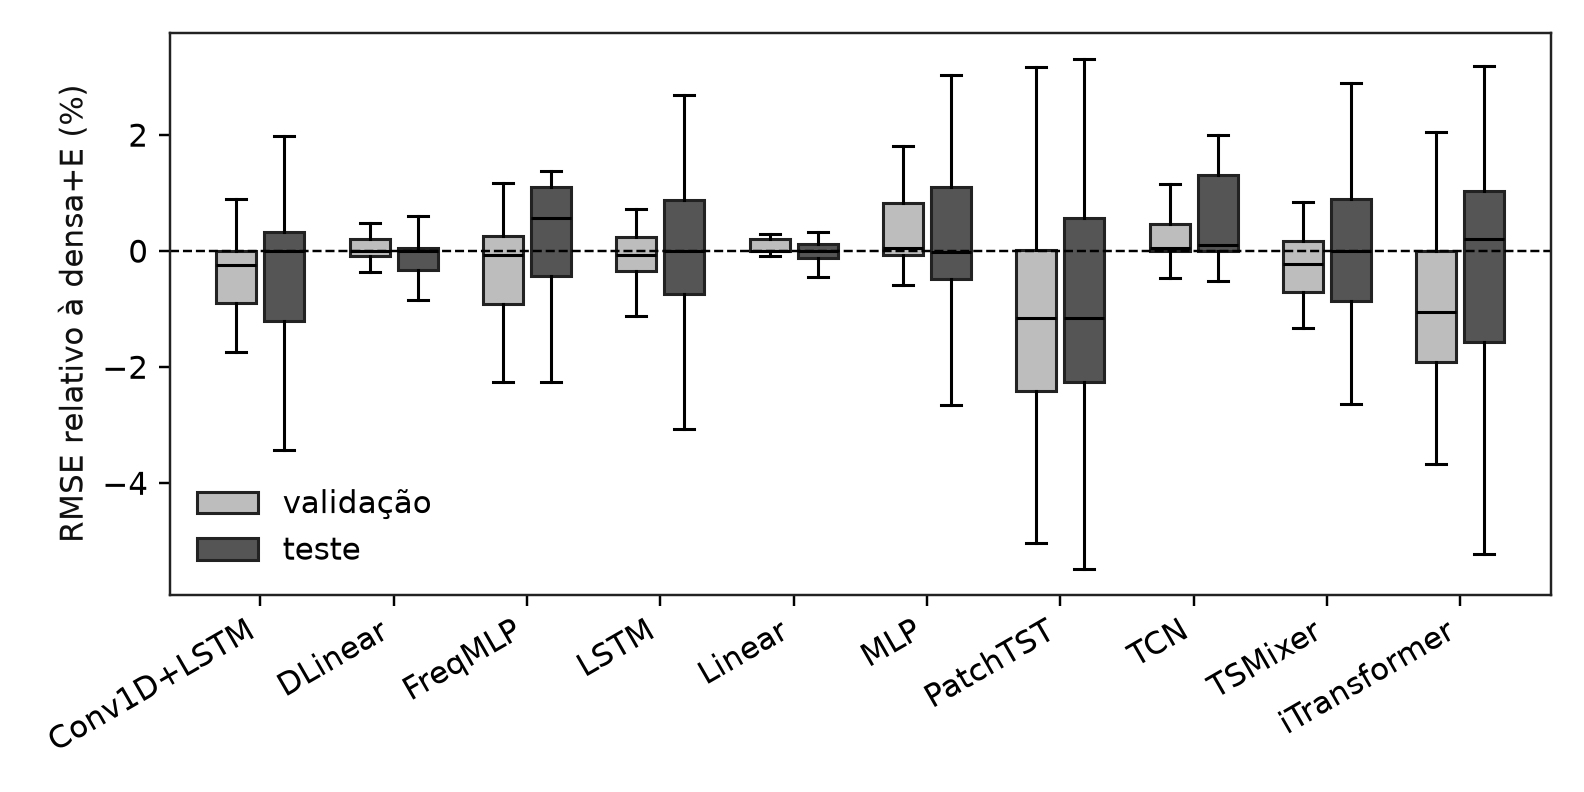
\includegraphics[width=0.92\linewidth]{figuras/t1_por_backbone.png}\par\smallskip{\scriptsize Fonte: resultados/t1.csv.}\end{figure}
\subsection{Qual variante NFH mais vence}
A Tabela~\ref{tab:t1_variantes} conta, para cada variante, em quantas combinações ela venceu a densa+E no RMSE de validação e no de teste (cada variante olhada sozinha) e quantas vezes foi a escolhida na validação. A que mais venceu no teste foi \texttt{conv\_L1000\_K10}, com 108 vitórias em 226 combinações; a mais escolhida na validação foi \texttt{conv\_L1000\_K10} (179 vezes). A Tabela~\ref{tab:t1_variantes_agr} agrega por família (\texttt{conv} = conversão exata da densa e ajuste; \texttt{zero} = NFH treinada do zero), por $\lambda$ e por $K$.

\begin{table}[htbp]
\centering
\scriptsize
\setlength{\tabcolsep}{2pt}
\caption{T1: variantes NFH, vit\'orias sobre a densa+E (RMSE) e escolhas pela valida\c{c}\~ao.}\label{tab:t1_variantes}
\begin{tabular}{lrrrrr}
\toprule
Variante & Comb. & \shortstack[l]{Vence val} & \shortstack[l]{Vence teste} & \shortstack[l]{Mediana rel.\\ RMSE teste} & Escolhida \\ \midrule
\texttt{conv\_L1000\_K10} & 226 & 115 & 108 & +0,00\% & 179 \\
\texttt{zero\_L100\_K10} & 226 & 50 & 55 & +1,45\% & 23 \\
\texttt{zero\_L1000\_K10} & 226 & 36 & 43 & +2,30\% & 16 \\
\texttt{zero\_L1000\_K4} & 60 & 14 & 13 & +3,59\% & 8 \\
\bottomrule
\end{tabular}
\par\smallskip{\scriptsize Fonte: resultados/t1.csv (semente 0, largura 1).}
\end{table}


\begin{table}[htbp]
\centering
\scriptsize
\setlength{\tabcolsep}{2pt}
\caption{T1: vit\'orias por fam\'ilia, $\lambda$ e $K$ (soma sobre as variantes do grupo).}\label{tab:t1_variantes_agr}
\begin{tabular}{llrrrr}
\toprule
Campo & Valor & Pares & \shortstack[l]{Vence val} & \shortstack[l]{Vence teste} & Escolhida \\ \midrule
família & conv & 226 & 115 & 108 & 179 \\
família & zero & 512 & 100 & 111 & 47 \\
$\lambda$ & 100.0 & 226 & 50 & 55 & 23 \\
$\lambda$ & 1000.0 & 512 & 165 & 164 & 203 \\
K & 10 & 678 & 201 & 206 & 218 \\
K & 4 & 60 & 14 & 13 & 8 \\
\bottomrule
\end{tabular}
\par\smallskip{\scriptsize Fonte: resultados/t1.csv.}
\end{table}


\section{Aprofundamento T2}
A Tabela~\ref{tab:t2_rel} mostra, para cada par (combinação, largura), a melhor variante pela média do RMSE de validação relativo à densa+E nas 3 sementes, e as médias das diferenças relativas na validação e no teste. A Tabela~\ref{tab:t2_abs} traz as médias absolutas de RMSE e MAE. ``Passa'' e ``Conf.'' vêm de \texttt{selecao\_T2.md}.

\tiny
\setlength{\tabcolsep}{2pt}
\begin{longtable}{llrrlrrrrrrll}
\caption{T2: m\'edias sobre as sementes 0, 1 e 2 da diferen\c{c}a relativa da melhor variante NFH (contra a densa+E, salvo a \'ultima coluna de teste).}\label{tab:t2_rel}\\
\toprule
Conjunto & Backbone & Fr. & L & Variante & \shortstack[l]{RMSE val} & \shortstack[l]{MAE val} & \shortstack[l]{Pior sem.\\ val} & \shortstack[l]{RMSE teste} & \shortstack[l]{MAE teste} & \shortstack[l]{RMSE teste\\ vs densa} & Passa & Conf. \\ \midrule
\endfirsthead
\toprule
Conjunto & Backbone & Fr. & L & Variante & \shortstack[l]{RMSE val} & \shortstack[l]{MAE val} & \shortstack[l]{Pior sem.\\ val} & \shortstack[l]{RMSE teste} & \shortstack[l]{MAE teste} & \shortstack[l]{RMSE teste\\ vs densa} & Passa & Conf. \\ \midrule
\endhead
\bottomrule
\multicolumn{13}{l}{\textit{Fonte: resultados/t2.csv e selecao\_T2.md.}}\\
\endlastfoot
SINT-M-M & iTransformer & 0.25 & 2 & \texttt{conv\_\allowbreak{}L1000\_\allowbreak{}K10} & \textminus{}9,89\% & \textminus{}6,41\% & \textminus{}7,29\% & \textminus{}7,24\% & \textminus{}6,08\% & \textminus{}7,95\% & sim & sim \\
ETTh1-M & PatchTST & 0.25 & 2 & \texttt{zero\_\allowbreak{}L1000\_\allowbreak{}K4} & \textminus{}8,66\% & \textminus{}7,06\% & \textminus{}7,66\% & \textminus{}5,91\% & \textminus{}0,99\% & \textminus{}5,91\% & sim & sim \\
ETTh1-M & PatchTST & 0.25 & 1 & \texttt{zero\_\allowbreak{}L1000\_\allowbreak{}K4} & \textminus{}6,98\% & \textminus{}5,54\% & \textminus{}3,70\% & \textminus{}4,32\% & \textminus{}0,33\% & \textminus{}4,68\% & sim & sim \\
SINT-M-M & PatchTST & 0.1 & 1 & \texttt{conv\_\allowbreak{}L1000\_\allowbreak{}K4} & \textminus{}5,61\% & \textminus{}5,38\% & \textminus{}3,98\% & \textminus{}7,61\% & \textminus{}7,88\% & \textminus{}7,61\% & sim & sim \\
ETTh1-M & iTransformer & 0.25 & 1 & \texttt{zero\_\allowbreak{}L1000\_\allowbreak{}K4} & \textminus{}5,47\% & \textminus{}5,10\% & \textminus{}4,36\% & \textminus{}0,95\% & +0,23\% & +0,22\% & sim & n\~ao \\
SINT-M-M & iTransformer & 0.25 & 1 & \texttt{conv\_\allowbreak{}L1000\_\allowbreak{}K10} & \textminus{}4,63\% & \textminus{}2,71\% & \textminus{}3,59\% & \textminus{}4,99\% & \textminus{}3,99\% & \textminus{}5,41\% & sim & n\~ao \\
air\_quality-U & PatchTST & 1 & 1 & \texttt{zero\_\allowbreak{}L1000\_\allowbreak{}K10} & \textminus{}4,31\% & \textminus{}4,77\% & \textminus{}3,47\% & +2,72\% & +0,32\% & +0,91\% & sim & n\~ao \\
SINT-M-M & PatchTST & 0.1 & 2 & \texttt{conv\_\allowbreak{}L1000\_\allowbreak{}K10} & \textminus{}3,80\% & \textminus{}3,29\% & \textminus{}2,98\% & \textminus{}4,99\% & \textminus{}4,61\% & \textminus{}4,99\% & sim & n\~ao \\
ETTh2-U & iTransformer & 0.25 & 1 & \texttt{zero\_\allowbreak{}L1000\_\allowbreak{}K4} & \textminus{}2,94\% & \textminus{}3,13\% & \textminus{}2,38\% & \textminus{}3,93\% & \textminus{}4,07\% & \textminus{}3,77\% & sim & sim \\
SINT-U48-U & Linear & 0.1 & 1 & \texttt{zero\_\allowbreak{}L1000\_\allowbreak{}K4} & \textminus{}2,53\% & \textminus{}2,48\% & \textminus{}2,37\% & \textminus{}2,53\% & \textminus{}2,22\% & \textminus{}2,74\% & sim & sim \\
SINT-M-M & Conv1D+LSTM & 1 & 2 & \texttt{zero\_\allowbreak{}L1000\_\allowbreak{}K10} & \textminus{}2,23\% & \textminus{}2,22\% & \textminus{}1,12\% & \textminus{}1,14\% & \textminus{}1,07\% & \textminus{}2,22\% & sim & n\~ao \\
SINT-U48-U & DLinear & 0.1 & 1 & \texttt{zero\_\allowbreak{}L1000\_\allowbreak{}K4} & \textminus{}2,13\% & \textminus{}2,14\% & \textminus{}2,06\% & \textminus{}2,17\% & \textminus{}2,02\% & \textminus{}2,48\% & sim & sim \\
SINT-M-M & Conv1D+LSTM & 1 & 1 & \texttt{conv\_\allowbreak{}L1000\_\allowbreak{}K4} & \textminus{}1,70\% & \textminus{}1,51\% & \textminus{}0,00\% & +0,92\% & +0,99\% & +1,71\% & sim & n\~ao \\
seoul\_bike-U & Conv1D+LSTM & 1 & 1 & \texttt{conv\_\allowbreak{}L1000\_\allowbreak{}K10} & \textminus{}1,62\% & \textminus{}1,22\% & +0,00\% & +0,37\% & +0,01\% & \textminus{}2,01\% & n\~ao & n\~ao \\
ETTh2-U & FreqMLP & 0.25 & 1 & \texttt{conv\_\allowbreak{}L100\_\allowbreak{}K10} & \textminus{}1,39\% & \textminus{}1,69\% & \textminus{}0,70\% & \textminus{}1,48\% & \textminus{}0,91\% & \textminus{}1,48\% & sim & sim \\
SINT-U48-U & FreqMLP & 0.1 & 1 & \texttt{zero\_\allowbreak{}L100\_\allowbreak{}K10} & \textminus{}0,27\% & \textminus{}0,02\% & +2,20\% & \textminus{}0,13\% & \textminus{}0,27\% & \textminus{}0,45\% & n\~ao & n\~ao \\
\end{longtable}
\normalsize


\tiny
\setlength{\tabcolsep}{2pt}
\begin{longtable}{llrrrrrrrrrr}
\caption{T2: m\'edias sobre as 3 sementes de RMSE e MAE (escala padronizada pelo treino).}\label{tab:t2_abs}\\
\toprule
Conjunto & Backbone & Fr. & L & \shortstack[l]{RMSE val\\ densa+E} & \shortstack[l]{RMSE val\\ NFH} & \shortstack[l]{RMSE teste\\ densa} & \shortstack[l]{RMSE teste\\ densa+E} & \shortstack[l]{RMSE teste\\ NFH} & \shortstack[l]{MAE teste\\ densa} & \shortstack[l]{MAE teste\\ densa+E} & \shortstack[l]{MAE teste\\ NFH} \\ \midrule
\endfirsthead
\toprule
Conjunto & Backbone & Fr. & L & \shortstack[l]{RMSE val\\ densa+E} & \shortstack[l]{RMSE val\\ NFH} & \shortstack[l]{RMSE teste\\ densa} & \shortstack[l]{RMSE teste\\ densa+E} & \shortstack[l]{RMSE teste\\ NFH} & \shortstack[l]{MAE teste\\ densa} & \shortstack[l]{MAE teste\\ densa+E} & \shortstack[l]{MAE teste\\ NFH} \\ \midrule
\endhead
\bottomrule
\multicolumn{12}{l}{\textit{Fonte: resultados/t2.csv.}}\\
\endlastfoot
SINT-M-M & iTransformer & 0.25 & 2 & 0,2853 & 0,2570 & 0,3178 & 0,3154 & 0,2925 & 0,2469 & 0,2448 & 0,2299 \\
ETTh1-M & PatchTST & 0.25 & 2 & 0,2615 & 0,2388 & 0,3343 & 0,3343 & 0,3145 & 0,2485 & 0,2485 & 0,2460 \\
ETTh1-M & PatchTST & 0.25 & 1 & 0,2549 & 0,2370 & 0,3245 & 0,3233 & 0,3089 & 0,2421 & 0,2409 & 0,2397 \\
SINT-M-M & PatchTST & 0.1 & 1 & 0,2756 & 0,2600 & 0,2896 & 0,2896 & 0,2671 & 0,2304 & 0,2304 & 0,2118 \\
ETTh1-M & iTransformer & 0.25 & 1 & 0,2469 & 0,2334 & 0,2956 & 0,2990 & 0,2961 & 0,2253 & 0,2270 & 0,2275 \\
SINT-M-M & iTransformer & 0.25 & 1 & 0,2732 & 0,2605 & 0,3103 & 0,3089 & 0,2935 & 0,2420 & 0,2401 & 0,2305 \\
air\_quality-U & PatchTST & 1 & 1 & 0,8486 & 0,8120 & 0,5925 & 0,5819 & 0,5977 & 0,4391 & 0,4320 & 0,4333 \\
SINT-M-M & PatchTST & 0.1 & 2 & 0,2671 & 0,2570 & 0,2816 & 0,2816 & 0,2675 & 0,2220 & 0,2220 & 0,2118 \\
ETTh2-U & iTransformer & 0.25 & 1 & 0,3502 & 0,3399 & 0,4884 & 0,4892 & 0,4700 & 0,3745 & 0,3754 & 0,3602 \\
SINT-U48-U & Linear & 0.1 & 1 & 0,3169 & 0,3089 & 0,3156 & 0,3149 & 0,3069 & 0,2503 & 0,2498 & 0,2443 \\
SINT-M-M & Conv1D+LSTM & 1 & 2 & 0,2180 & 0,2131 & 0,2388 & 0,2363 & 0,2335 & 0,1890 & 0,1865 & 0,1845 \\
SINT-U48-U & DLinear & 0.1 & 1 & 0,3152 & 0,3085 & 0,3140 & 0,3130 & 0,3063 & 0,2492 & 0,2484 & 0,2434 \\
SINT-M-M & Conv1D+LSTM & 1 & 1 & 0,2167 & 0,2130 & 0,2249 & 0,2266 & 0,2287 & 0,1770 & 0,1783 & 0,1801 \\
seoul\_bike-U & Conv1D+LSTM & 1 & 1 & 0,9062 & 0,8914 & 0,6247 & 0,6099 & 0,6121 & 0,4396 & 0,4227 & 0,4228 \\
ETTh2-U & FreqMLP & 0.25 & 1 & 0,3583 & 0,3533 & 0,4961 & 0,4961 & 0,4887 & 0,3835 & 0,3835 & 0,3800 \\
SINT-U48-U & FreqMLP & 0.1 & 1 & 0,3371 & 0,3362 & 0,3420 & 0,3409 & 0,3404 & 0,2731 & 0,2724 & 0,2716 \\
\end{longtable}
\normalsize


\section{Confirmação com sementes novas}
As Tabelas~\ref{tab:conf_rmse} e \ref{tab:conf_mae} dão, por combinação, a média $\pm$ desvio-padrão amostral (denominador $n-1$) entre as sementes de RMSE e MAE de teste da densa, da densa+E, da \texttt{proj\_K10} e da NFH. A Tabela~\ref{tab:conf_vit} traz as vitórias da NFH por semente (estritamente menor), a comparação com a melhor ingênua (média de treino, último valor ou sazonal de 24 h, a de menor erro de teste em cada métrica) e o veredito pelo critério do \S{}6.

\textbf{Atenção:} a linha marcada com $\dagger$ é o exemplo passo a passo, com \textbf{outro protocolo}: $H=8$, série de livro, 10 sementes (10 e 19), critério com pelo menos 8 vitórias, sem \texttt{proj\_K10} nem ingênuas. Ela não é comparável às demais.

\textbf{O que as sementes variam, e o que não.} Na T1, na T2 e na confirmação, a semente muda só a inicialização dos pesos e a ordem dos lotes. A divisão cronológica (70/15/15) e as séries sintéticas são fixas, e a confirmação avalia o \emph{mesmo bloco de teste} da T1 e da T2: as sementes são novas, o teste não. O desvio-padrão das tabelas mede, portanto, a variação do treino, e \emph{não} mede a incerteza de amostragem do teste. Ganhos pequenos podem não se repetir em outra série ou em outro bloco de teste.

\tiny
\setlength{\tabcolsep}{2pt}
\begin{longtable}{llrrlrrllll}
\caption{Confirma\c{c}\~ao: RMSE de teste, m\'edia $\pm$ desvio-padr\~ao entre as sementes (escala padronizada pelo treino; menor \'e melhor). A coluna ``Sem. com densa+E = densa'' conta as sementes em que a \'epoca escolhida da densa+E \'e 0, isto \'e, a densa+E \'e o mesmo modelo da densa.}\label{tab:conf_rmse}\\
\toprule
Conjunto & Backbone & Fr. & L & \shortstack[l]{Variante NFH} & Sem. & \shortstack[l]{Sem. com\\ densa+E =\\ densa (época\\ 0)} & densa & densa+E & proj\_K10 & NFH \\ \midrule
\endfirsthead
\toprule
Conjunto & Backbone & Fr. & L & \shortstack[l]{Variante NFH} & Sem. & \shortstack[l]{Sem. com\\ densa+E =\\ densa (época\\ 0)} & densa & densa+E & proj\_K10 & NFH \\ \midrule
\endhead
\bottomrule
\multicolumn{11}{l}{\textit{Fonte: resultados/confirmacao.csv; $\dagger$ = exemplo\_sintetico/confirmacao.csv (outro protocolo, $H=8$).}}\\
\endlastfoot
ETTh1-M & PatchTST & 0.25 & 1 & \texttt{zero\_\allowbreak{}L1000\_\allowbreak{}K4} & 5 & 2/5 & 0,3255 $\pm$ 0,0091 & 0,3207 $\pm$ 0,0073 & 0,3236 $\pm$ 0,0094 & 0,3080 $\pm$ 0,0032 \\
ETTh1-M & PatchTST & 0.25 & 2 & \texttt{zero\_\allowbreak{}L1000\_\allowbreak{}K4} & 5 & 4/5 & 0,3246 $\pm$ 0,0110 & 0,3219 $\pm$ 0,0117 & 0,3236 $\pm$ 0,0107 & 0,3129 $\pm$ 0,0025 \\
ETTh2-U & FreqMLP & 0.25 & 1 & \texttt{conv\_\allowbreak{}L100\_\allowbreak{}K10} & 5 & 2/5 & 0,4962 $\pm$ 0,0098 & 0,4951 $\pm$ 0,0089 & 0,4914 $\pm$ 0,0102 & 0,4876 $\pm$ 0,0066 \\
ETTh2-U & iTransformer & 0.25 & 1 & \texttt{zero\_\allowbreak{}L1000\_\allowbreak{}K4} & 5 & 5/5 & 0,4898 $\pm$ 0,0161 & 0,4898 $\pm$ 0,0161 & 0,4895 $\pm$ 0,0162 & 0,4752 $\pm$ 0,0038 \\
SINT-M-M & PatchTST & 0.1 & 1 & \texttt{conv\_\allowbreak{}L1000\_\allowbreak{}K4} & 5 & 4/5 & 0,2923 $\pm$ 0,0116 & 0,2923 $\pm$ 0,0116 & 0,2898 $\pm$ 0,0115 & 0,2695 $\pm$ 0,0091 \\
SINT-M-M & iTransformer & 0.25 & 2 & \texttt{conv\_\allowbreak{}L1000\_\allowbreak{}K10} & 5 & 2/5 & 0,3173 $\pm$ 0,0104 & 0,3144 $\pm$ 0,0095 & 0,3166 $\pm$ 0,0102 & 0,2949 $\pm$ 0,0051 \\
SINT-U48-U & DLinear & 0.1 & 1 & \texttt{zero\_\allowbreak{}L1000\_\allowbreak{}K4} & 5 & 0/5 & 0,3140 $\pm$ 0,0001 & 0,3132 $\pm$ 0,0001 & 0,3096 $\pm$ 0,0002 & 0,3073 $\pm$ 0,0009 \\
SINT-U48-U & Linear & 0.1 & 1 & \texttt{zero\_\allowbreak{}L1000\_\allowbreak{}K4} & 5 & 0/5 & 0,3155 $\pm$ 0,0004 & 0,3148 $\pm$ 0,0001 & 0,3101 $\pm$ 0,0003 & 0,3063 $\pm$ 0,0003 \\
SINT-H8 (livro)$^\dagger$ & 1 camada, p=16 & n=1000 & -- & \texttt{zero\_\allowbreak{}L1000} & 10 & n/d & 0,3282 $\pm$ 0,0116 & 0,3285 $\pm$ 0,0124 & n/d & 0,3038 $\pm$ 0,0015 \\
\end{longtable}
\normalsize


\tiny
\setlength{\tabcolsep}{2pt}
\begin{longtable}{llrrllll}
\caption{Confirma\c{c}\~ao: MAE de teste, m\'edia $\pm$ desvio-padr\~ao entre as sementes.}\label{tab:conf_mae}\\
\toprule
Conjunto & Backbone & Fr. & L & densa & densa+E & proj\_K10 & NFH \\ \midrule
\endfirsthead
\toprule
Conjunto & Backbone & Fr. & L & densa & densa+E & proj\_K10 & NFH \\ \midrule
\endhead
\bottomrule
\multicolumn{8}{l}{\textit{Fonte: resultados/confirmacao.csv; $\dagger$ = exemplo (outro protocolo).}}\\
\endlastfoot
ETTh1-M & PatchTST & 0.25 & 1 & 0,2425 $\pm$ 0,0098 & 0,2390 $\pm$ 0,0047 & 0,2409 $\pm$ 0,0101 & 0,2405 $\pm$ 0,0033 \\
ETTh1-M & PatchTST & 0.25 & 2 & 0,2424 $\pm$ 0,0079 & 0,2397 $\pm$ 0,0083 & 0,2415 $\pm$ 0,0076 & 0,2447 $\pm$ 0,0026 \\
ETTh2-U & FreqMLP & 0.25 & 1 & 0,3829 $\pm$ 0,0097 & 0,3813 $\pm$ 0,0085 & 0,3791 $\pm$ 0,0102 & 0,3787 $\pm$ 0,0051 \\
ETTh2-U & iTransformer & 0.25 & 1 & 0,3732 $\pm$ 0,0146 & 0,3732 $\pm$ 0,0146 & 0,3729 $\pm$ 0,0146 & 0,3654 $\pm$ 0,0039 \\
SINT-M-M & PatchTST & 0.1 & 1 & 0,2309 $\pm$ 0,0083 & 0,2309 $\pm$ 0,0083 & 0,2291 $\pm$ 0,0082 & 0,2133 $\pm$ 0,0072 \\
SINT-M-M & iTransformer & 0.25 & 2 & 0,2465 $\pm$ 0,0075 & 0,2449 $\pm$ 0,0078 & 0,2459 $\pm$ 0,0075 & 0,2306 $\pm$ 0,0040 \\
SINT-U48-U & DLinear & 0.1 & 1 & 0,2490 $\pm$ 0,0001 & 0,2485 $\pm$ 0,0001 & 0,2455 $\pm$ 0,0001 & 0,2444 $\pm$ 0,0007 \\
SINT-U48-U & Linear & 0.1 & 1 & 0,2502 $\pm$ 0,0004 & 0,2497 $\pm$ 0,0001 & 0,2459 $\pm$ 0,0003 & 0,2436 $\pm$ 0,0003 \\
SINT-H8 (livro)$^\dagger$ & 1 camada, p=16 & n=1000 & -- & 0,2625 $\pm$ 0,0088 & 0,2625 $\pm$ 0,0093 & n/d & 0,2445 $\pm$ 0,0011 \\
\end{longtable}
\normalsize


\tiny
\setlength{\tabcolsep}{2pt}
\begin{longtable}{llrrrrrrlrrl}
\caption{Confirma\c{c}\~ao: vit\'orias da NFH por semente (estritamente menor), compara\c{c}\~ao com a melhor ing\^enua e veredito do \S6.}\label{tab:conf_vit}\\
\toprule
Conjunto & Backbone & Fr. & L & \shortstack[l]{RMSE vs\\ densa+E} & \shortstack[l]{MAE vs\\ densa+E} & \shortstack[l]{RMSE vs\\ densa} & \shortstack[l]{MAE vs\\ densa} & \shortstack[l]{Melhor ing\^enua\\ (RMSE)} & \shortstack[l]{NFH vs\\ ing. RMSE} & \shortstack[l]{NFH vs\\ ing. MAE} & Veredito \\ \midrule
\endfirsthead
\toprule
Conjunto & Backbone & Fr. & L & \shortstack[l]{RMSE vs\\ densa+E} & \shortstack[l]{MAE vs\\ densa+E} & \shortstack[l]{RMSE vs\\ densa} & \shortstack[l]{MAE vs\\ densa} & \shortstack[l]{Melhor ing\^enua\\ (RMSE)} & \shortstack[l]{NFH vs\\ ing. RMSE} & \shortstack[l]{NFH vs\\ ing. MAE} & Veredito \\ \midrule
\endhead
\bottomrule
\multicolumn{12}{l}{\textit{Fonte: resultados/confirmacao.csv (ing\^enuas: linhas \texttt{ingenua\_*}); $\dagger$ = exemplo (outro protocolo).}}\\
\endlastfoot
ETTh1-M & PatchTST & 0.25 & 1 & 5/5 & 2/5 & 5/5 & 2/5 & 0,3013 (ulti) & +2,22\% & +6,78\% & \textbf{FALHA} \\
ETTh1-M & PatchTST & 0.25 & 2 & 4/5 & 2/5 & 4/5 & 3/5 & 0,3013 (ulti) & +3,85\% & +8,61\% & \textbf{FALHA} \\
ETTh2-U & FreqMLP & 0.25 & 1 & 5/5 & 4/5 & 5/5 & 4/5 & 0,5188 (sazo) & \textminus{}6,02\% & \textminus{}2,56\% & \textbf{SUCESSO} \\
ETTh2-U & iTransformer & 0.25 & 1 & 5/5 & 4/5 & 5/5 & 4/5 & 0,5188 (sazo) & \textminus{}8,41\% & \textminus{}5,98\% & \textbf{SUCESSO} \\
SINT-M-M & PatchTST & 0.1 & 1 & 5/5 & 5/5 & 5/5 & 5/5 & 0,3850 (sazo) & \textminus{}30,00\% & \textminus{}30,08\% & \textbf{SUCESSO} \\
SINT-M-M & iTransformer & 0.25 & 2 & 5/5 & 5/5 & 5/5 & 5/5 & 0,3850 (sazo) & \textminus{}23,41\% & \textminus{}24,39\% & \textbf{SUCESSO} \\
SINT-U48-U & DLinear & 0.1 & 1 & 5/5 & 5/5 & 5/5 & 5/5 & 0,3927 (sazo) & \textminus{}21,74\% & \textminus{}22,38\% & \textbf{SUCESSO} \\
SINT-U48-U & Linear & 0.1 & 1 & 5/5 & 5/5 & 5/5 & 5/5 & 0,3927 (sazo) & \textminus{}21,99\% & \textminus{}22,64\% & \textbf{SUCESSO} \\
SINT-H8 (livro)$^\dagger$ & 1 camada, p=16 & n=1000 & -- & 10/10 & 10/10 & 10/10 & 10/10 & n/d & n/d & n/d & \textbf{SUCESSO}$^\dagger$ \\
\end{longtable}
\normalsize


\textbf{Controle das épocas extras sem efeito em parte das sementes.} Quando a época escolhida da densa+E é 0, as 15 épocas extras não melhoraram a validação e a densa+E é o mesmo modelo da densa (RMSE de teste igual nessas sementes). Isso ocorre, em número de sementes, em: ETTh1-M/PatchTST (largura 1): 2 de 5; ETTh1-M/PatchTST (largura 2): 4 de 5; ETTh2-U/FreqMLP (largura 1): 2 de 5; ETTh2-U/iTransformer (largura 1): 5 de 5; SINT-M/PatchTST (largura 1): 4 de 5; SINT-M/iTransformer (largura 2): 2 de 5. Nessas sementes o controle não acrescenta informação; a comparação continua válida, porque a NFH é comparada com o melhor que a densa conseguiu na validação, mas a coluna da densa+E repete a da densa.

\begin{figure}[htbp]\centering\caption{Confirmação: RMSE de teste da NFH relativo à densa+E, por semente (pontos cinza) e na média (losango preto). Valores negativos favorecem a NFH.}\label{fig:conf}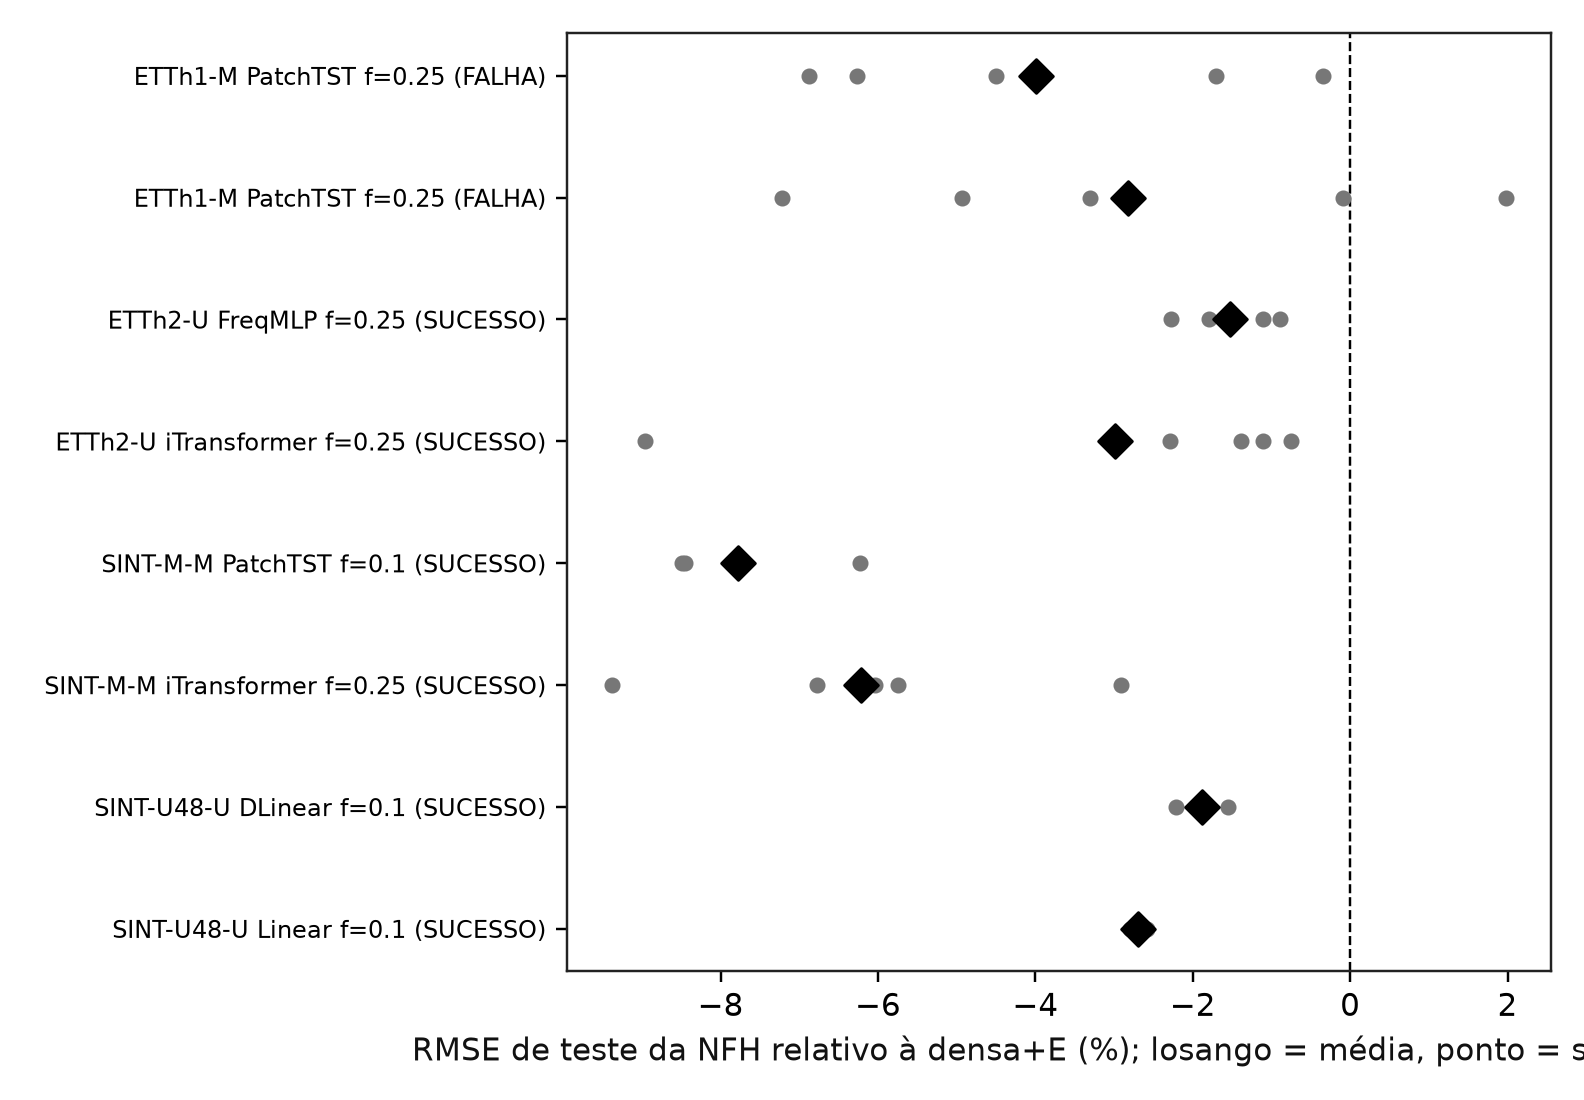
\includegraphics[width=0.95\linewidth]{figuras/confirmacao_por_semente.png}\par\smallskip{\scriptsize Fonte: resultados/confirmacao.csv.}\end{figure}
\section{Exemplos em que a NFH iguala ou supera a densa}\label{sec:exemplos}
Esta seção lista \emph{somente} as combinações com SUCESSO: média de RMSE e de MAE de teste da NFH menores ou iguais às da densa e da densa+E, e vitória em RMSE contra a densa+E em pelo menos 4 das 5 sementes. Elas foram \emph{procuradas} (T1, T2 e confirmação) e não representam o comportamento geral.

\paragraph{ETTh2-U, FreqMLP, fração 0.25, largura 1, variante \texttt{conv\_\allowbreak{}L100\_\allowbreak{}K10}.} RMSE de teste (média $\pm$ dp, 5 sementes): NFH 0,4876 $\pm$ 0,0066; densa 0,4962 $\pm$ 0,0098; densa+E 0,4951 $\pm$ 0,0089; \texttt{proj\_K10} 0,4914 $\pm$ 0,0102. MAE de teste: NFH 0,3787 $\pm$ 0,0051; densa 0,3829 $\pm$ 0,0097; densa+E 0,3813 $\pm$ 0,0085. A diferença relativa das médias da NFH é \textminus{}1,52\% (RMSE) e \textminus{}0,68\% (MAE) contra a densa+E, e \textminus{}1,74\% e \textminus{}1,09\% contra a densa. Vitórias da NFH: RMSE 5 de 5 e MAE 4 de 5 contra a densa+E; RMSE 5 e MAE 4 contra a densa. Cobertura mediana $1-\varepsilon_R$ da NFH: 0,996. 
Melhor ingênua em RMSE: ingenua\_sazonal24 (0,5188); a NFH fica \textminus{}6,02\% dela em RMSE e \textminus{}2,56\% em MAE (melhor ingênua em MAE: ingenua\_sazonal24). A densa fica \textminus{}4,35\% da melhor ingênua em RMSE.


\paragraph{ETTh2-U, iTransformer, fração 0.25, largura 1, variante \texttt{zero\_\allowbreak{}L1000\_\allowbreak{}K4}.} RMSE de teste (média $\pm$ dp, 5 sementes): NFH 0,4752 $\pm$ 0,0038; densa 0,4898 $\pm$ 0,0161; densa+E 0,4898 $\pm$ 0,0161; \texttt{proj\_K10} 0,4895 $\pm$ 0,0162. MAE de teste: NFH 0,3654 $\pm$ 0,0039; densa 0,3732 $\pm$ 0,0146; densa+E 0,3732 $\pm$ 0,0146. A diferença relativa das médias da NFH é \textminus{}2,99\% (RMSE) e \textminus{}2,07\% (MAE) contra a densa+E, e \textminus{}2,99\% e \textminus{}2,07\% contra a densa. Vitórias da NFH: RMSE 5 de 5 e MAE 4 de 5 contra a densa+E; RMSE 5 e MAE 4 contra a densa. Cobertura mediana $1-\varepsilon_R$ da NFH: 1,000. 
Melhor ingênua em RMSE: ingenua\_sazonal24 (0,5188); a NFH fica \textminus{}8,41\% dela em RMSE e \textminus{}5,98\% em MAE (melhor ingênua em MAE: ingenua\_sazonal24). A densa fica \textminus{}5,58\% da melhor ingênua em RMSE.


\paragraph{SINT-M-M, PatchTST, fração 0.1, largura 1, variante \texttt{conv\_\allowbreak{}L1000\_\allowbreak{}K4}.} RMSE de teste (média $\pm$ dp, 5 sementes): NFH 0,2695 $\pm$ 0,0091; densa 0,2923 $\pm$ 0,0116; densa+E 0,2923 $\pm$ 0,0116; \texttt{proj\_K10} 0,2898 $\pm$ 0,0115. MAE de teste: NFH 0,2133 $\pm$ 0,0072; densa 0,2309 $\pm$ 0,0083; densa+E 0,2309 $\pm$ 0,0083. A diferença relativa das médias da NFH é \textminus{}7,78\% (RMSE) e \textminus{}7,65\% (MAE) contra a densa+E, e \textminus{}7,78\% e \textminus{}7,65\% contra a densa. Vitórias da NFH: RMSE 5 de 5 e MAE 5 de 5 contra a densa+E; RMSE 5 e MAE 5 contra a densa. Cobertura mediana $1-\varepsilon_R$ da NFH: 1,000. 
Melhor ingênua em RMSE: ingenua\_sazonal24 (0,3850); a NFH fica \textminus{}30,00\% dela em RMSE e \textminus{}30,08\% em MAE (melhor ingênua em MAE: ingenua\_sazonal24). A densa fica \textminus{}24,09\% da melhor ingênua em RMSE.


\paragraph{SINT-M-M, iTransformer, fração 0.25, largura 2, variante \texttt{conv\_\allowbreak{}L1000\_\allowbreak{}K10}.} RMSE de teste (média $\pm$ dp, 5 sementes): NFH 0,2949 $\pm$ 0,0051; densa 0,3173 $\pm$ 0,0104; densa+E 0,3144 $\pm$ 0,0095; \texttt{proj\_K10} 0,3166 $\pm$ 0,0102. MAE de teste: NFH 0,2306 $\pm$ 0,0040; densa 0,2465 $\pm$ 0,0075; densa+E 0,2449 $\pm$ 0,0078. A diferença relativa das médias da NFH é \textminus{}6,22\% (RMSE) e \textminus{}5,84\% (MAE) contra a densa+E, e \textminus{}7,08\% e \textminus{}6,46\% contra a densa. Vitórias da NFH: RMSE 5 de 5 e MAE 5 de 5 contra a densa+E; RMSE 5 e MAE 5 contra a densa. Cobertura mediana $1-\varepsilon_R$ da NFH: 1,000. 
Melhor ingênua em RMSE: ingenua\_sazonal24 (0,3850); a NFH fica \textminus{}23,41\% dela em RMSE e \textminus{}24,39\% em MAE (melhor ingênua em MAE: ingenua\_sazonal24). A densa fica \textminus{}17,58\% da melhor ingênua em RMSE.


\paragraph{SINT-U48-U, DLinear, fração 0.1, largura 1, variante \texttt{zero\_\allowbreak{}L1000\_\allowbreak{}K4}.} RMSE de teste (média $\pm$ dp, 5 sementes): NFH 0,3073 $\pm$ 0,0009; densa 0,3140 $\pm$ 0,0001; densa+E 0,3132 $\pm$ 0,0001; \texttt{proj\_K10} 0,3096 $\pm$ 0,0002. MAE de teste: NFH 0,2444 $\pm$ 0,0007; densa 0,2490 $\pm$ 0,0001; densa+E 0,2485 $\pm$ 0,0001. A diferença relativa das médias da NFH é \textminus{}1,89\% (RMSE) e \textminus{}1,64\% (MAE) contra a densa+E, e \textminus{}2,12\% e \textminus{}1,85\% contra a densa. Vitórias da NFH: RMSE 5 de 5 e MAE 5 de 5 contra a densa+E; RMSE 5 e MAE 5 contra a densa. Cobertura mediana $1-\varepsilon_R$ da NFH: 1,000. 
Melhor ingênua em RMSE: ingenua\_sazonal24 (0,3927); a NFH fica \textminus{}21,74\% dela em RMSE e \textminus{}22,38\% em MAE (melhor ingênua em MAE: ingenua\_sazonal24). A densa fica \textminus{}20,04\% da melhor ingênua em RMSE.


\paragraph{SINT-U48-U, Linear, fração 0.1, largura 1, variante \texttt{zero\_\allowbreak{}L1000\_\allowbreak{}K4}.} RMSE de teste (média $\pm$ dp, 5 sementes): NFH 0,3063 $\pm$ 0,0003; densa 0,3155 $\pm$ 0,0004; densa+E 0,3148 $\pm$ 0,0001; \texttt{proj\_K10} 0,3101 $\pm$ 0,0003. MAE de teste: NFH 0,2436 $\pm$ 0,0003; densa 0,2502 $\pm$ 0,0004; densa+E 0,2497 $\pm$ 0,0001. A diferença relativa das médias da NFH é \textminus{}2,70\% (RMSE) e \textminus{}2,46\% (MAE) contra a densa+E, e \textminus{}2,91\% e \textminus{}2,63\% contra a densa. Vitórias da NFH: RMSE 5 de 5 e MAE 5 de 5 contra a densa+E; RMSE 5 e MAE 5 contra a densa. Cobertura mediana $1-\varepsilon_R$ da NFH: 1,000. 
Melhor ingênua em RMSE: ingenua\_sazonal24 (0,3927); a NFH fica \textminus{}21,99\% dela em RMSE e \textminus{}22,64\% em MAE (melhor ingênua em MAE: ingenua\_sazonal24). A densa fica \textminus{}19,65\% da melhor ingênua em RMSE.


\paragraph{Exemplo passo a passo (outro protocolo).} O exemplo didático ($H=8$, $p=16$, $n=1000$ janelas de treino, variante \texttt{zero\_\allowbreak{}L1000}) tem veredito SUCESSO no seu próprio critério (10 sementes, pelo menos 8 vitórias): RMSE de teste 0,3038 $\pm$ 0,0015 (NFH), 0,3282 $\pm$ 0,0116 (densa) e 0,3285 $\pm$ 0,0124 (densa+E). Foi avaliado no próprio protocolo (sem as ingênuas nem a \texttt{proj\_K10}); não é uma das combinações da T1, da T2 ou da confirmação de \emph{backbones}.

\section{Onde a NFH não ganhou}\label{sec:naoganhou}
\emph{Derrota}: a média de RMSE de teste da NFH é maior que a da densa ou a da densa+E. \emph{Falha pelo MAE}: as médias de RMSE não pioram, mas a média de MAE de teste da NFH é maior que a da densa ou a da densa+E; é uma derrota parcial. \emph{Falha pelas vitórias}: as médias de RMSE e de MAE não pioram, mas a NFH vence a densa+E em menos sementes que o mínimo. Não há limiar de tolerância, e este relatório não chama nenhuma combinação de empate.

\tiny
\setlength{\tabcolsep}{2pt}
\begin{longtable}{llrrllrrrlp{3.6cm}}
\caption{Confirma\c{c}\~ao: combina\c{c}\~oes sem SUCESSO (diferen\c{c}as relativas das m\'edias de teste).}\label{tab:nao_ganhou_conf}\\
\toprule
Conjunto & Backbone & Fr. & L & Variante & Tipo & \shortstack[l]{RMSE vs\\ densa+E} & \shortstack[l]{MAE vs\\ densa+E} & \shortstack[l]{RMSE vs\\ densa} & \shortstack[l]{Vit. RMSE} & \shortstack[l]{Falhas do\\ crit\'erio} \\ \midrule
\endfirsthead
\toprule
Conjunto & Backbone & Fr. & L & Variante & Tipo & \shortstack[l]{RMSE vs\\ densa+E} & \shortstack[l]{MAE vs\\ densa+E} & \shortstack[l]{RMSE vs\\ densa} & \shortstack[l]{Vit. RMSE} & \shortstack[l]{Falhas do\\ crit\'erio} \\ \midrule
\endhead
\bottomrule
\multicolumn{11}{l}{\textit{Fonte: resultados/confirmacao.csv.}}\\
\endlastfoot
ETTh1-M & PatchTST & 0.25 & 1 & \texttt{zero\_\allowbreak{}L1000\_\allowbreak{}K4} & falha pelo MAE & \textminus{}3,99\% & +0,65\% & \textminus{}5,39\% & 5/5 & média de MAE da NFH maior que a da densa+E \\
ETTh1-M & PatchTST & 0.25 & 2 & \texttt{zero\_\allowbreak{}L1000\_\allowbreak{}K4} & falha pelo MAE & \textminus{}2,82\% & +2,05\% & \textminus{}3,61\% & 4/5 & média de MAE da NFH maior que a da densa; média de MAE da NFH maior que a da densa+E \\
\end{longtable}
\normalsize


Em ETTh1-M/PatchTST (largura 1), fração 0,25: \textbf{todos os modelos ficam acima da ingênua do último valor}: RMSE médio de teste de 0,3013 para a ingênua contra 0,3080 (NFH), 0,3255 (densa) e 0,3207 (densa+E) e, no MAE, 0,2253 contra 0,2405 da NFH. A NFH não bate nem a ingênua nessa combinação; a diferença para a densa+E não muda isso.

Em ETTh1-M/PatchTST (largura 2), fração 0,25: \textbf{todos os modelos ficam acima da ingênua do último valor}: RMSE médio de teste de 0,3013 para a ingênua contra 0,3129 (NFH), 0,3246 (densa) e 0,3219 (densa+E) e, no MAE, 0,2253 contra 0,2447 da NFH. A NFH não bate nem a ingênua nessa combinação; a diferença para a densa+E não muda isso.

Na T2, 2 dos 16 pares (combinação, largura) não qualificaram para a confirmação (Tabela~\ref{tab:nao_ganhou_t2}).

\tiny
\setlength{\tabcolsep}{2pt}
\begin{longtable}{llrrlrrrrr}
\caption{T2: pares sem qualifica\c{c}\~ao (m\'edias sobre as sementes; contra a densa+E).}\label{tab:nao_ganhou_t2}\\
\toprule
Conjunto & Backbone & Fr. & L & Variante & \shortstack[l]{RMSE val} & \shortstack[l]{MAE val} & \shortstack[l]{Pior sem.\\ val} & \shortstack[l]{RMSE teste} & \shortstack[l]{MAE teste} \\ \midrule
\endfirsthead
\toprule
Conjunto & Backbone & Fr. & L & Variante & \shortstack[l]{RMSE val} & \shortstack[l]{MAE val} & \shortstack[l]{Pior sem.\\ val} & \shortstack[l]{RMSE teste} & \shortstack[l]{MAE teste} \\ \midrule
\endhead
\bottomrule
\multicolumn{10}{l}{\textit{Fonte: resultados/t2.csv.}}\\
\endlastfoot
seoul\_bike-U & Conv1D+LSTM & 1 & 1 & \texttt{conv\_\allowbreak{}L1000\_\allowbreak{}K10} & \textminus{}1,62\% & \textminus{}1,22\% & +0,00\% & +0,37\% & +0,01\% \\
SINT-U48-U & FreqMLP & 0.1 & 1 & \texttt{zero\_\allowbreak{}L100\_\allowbreak{}K10} & \textminus{}0,27\% & \textminus{}0,02\% & +2,20\% & \textminus{}0,13\% & \textminus{}0,27\% \\
\end{longtable}
\normalsize


Também na T2, 6 pares qualificaram pela validação e não foram à confirmação (limites da seleção da T2); 3 deles tiveram RMSE ou MAE de teste médio \emph{pior} que o da densa+E (Tabela~\ref{tab:t2_qualif_perdeu}). Eles não passaram pela confirmação, e a perda no teste da T2 é média de 3 sementes, sem sementes novas.

\tiny
\setlength{\tabcolsep}{2pt}
\begin{longtable}{llrrlrrrrl}
\caption{T2: pares que qualificaram, n\~ao foram \`a confirma\c{c}\~ao e perderam no teste (m\'edias sobre as sementes; contra a densa+E).}\label{tab:t2_qualif_perdeu}\\
\toprule
Conjunto & Backbone & Fr. & L & Variante & \shortstack[l]{RMSE val} & \shortstack[l]{MAE val} & \shortstack[l]{RMSE teste} & \shortstack[l]{MAE teste} & \shortstack[l]{Pior em} \\ \midrule
\endfirsthead
\toprule
Conjunto & Backbone & Fr. & L & Variante & \shortstack[l]{RMSE val} & \shortstack[l]{MAE val} & \shortstack[l]{RMSE teste} & \shortstack[l]{MAE teste} & \shortstack[l]{Pior em} \\ \midrule
\endhead
\bottomrule
\multicolumn{10}{l}{\textit{Fonte: resultados/t2.csv e selecao\_T2.md.}}\\
\endlastfoot
ETTh1-M & iTransformer & 0.25 & 1 & \texttt{zero\_\allowbreak{}L1000\_\allowbreak{}K4} & \textminus{}5,47\% & \textminus{}5,10\% & \textminus{}0,95\% & +0,23\% & MAE \\
air\_quality-U & PatchTST & 1 & 1 & \texttt{zero\_\allowbreak{}L1000\_\allowbreak{}K10} & \textminus{}4,31\% & \textminus{}4,77\% & +2,72\% & +0,32\% & RMSE e MAE \\
SINT-M-M & Conv1D+LSTM & 1 & 1 & \texttt{conv\_\allowbreak{}L1000\_\allowbreak{}K4} & \textminus{}1,70\% & \textminus{}1,51\% & +0,92\% & +0,99\% & RMSE e MAE \\
\end{longtable}
\normalsize


Na T1, a melhor variante NFH não venceu a densa+E em RMSE de validação em 97 das 226 combinações e não a venceu em RMSE de teste em 114. A mediana da diferença relativa de RMSE de teste da melhor variante é +0,00\% contra a densa+E e \textminus{}0,06\% contra a densa. Todas as combinações da T1 estão no Apêndice~\ref{ap:t1}.

\section{Explicações das combinações com SUCESSO}
Esta seção só inclui as combinações cujo veredito recalculado a partir de \texttt{confirmacao.csv} é SUCESSO; o campo de veredito gravado nos arquivos de explicação não é usado para essa escolha.

Para 6 combinações, \texttt{explicar\_bb.py} usou o modelo da semente 10 salvo pela confirmação e calculou, no teste, a decomposição $T$, $S$, $R$, as participações $\varepsilon_T,\varepsilon_S,\varepsilon_R$ (mediana e quartis), a decomposição pura da densa pelo Projetor e os Integrated Gradients de $g_T$ e $g_S$ (referência zero) com o erro de completude.

\tiny
\setlength{\tabcolsep}{2pt}
\begin{longtable}{lllllrr}
\caption{Explica\c{c}\~oes (semente 10, teste): participa\c{c}\~oes de energia, mediana [Q1; Q3], e erro relativo mediano de completude dos IG (s\'o NFH).}\label{tab:expl_eps}\\
\toprule
Combina\c{c}\~ao & Modelo & $\varepsilon_T$ & $\varepsilon_S$ & $\varepsilon_R$ & \shortstack[l]{Compl. $g_T$} & \shortstack[l]{Compl. $g_S$} \\ \midrule
\endfirsthead
\toprule
Combina\c{c}\~ao & Modelo & $\varepsilon_T$ & $\varepsilon_S$ & $\varepsilon_R$ & \shortstack[l]{Compl. $g_T$} & \shortstack[l]{Compl. $g_S$} \\ \midrule
\endhead
\bottomrule
\multicolumn{7}{l}{\textit{Fonte: resultados/explicacoes/*.json.}}\\
\endlastfoot
ETTh2\_\allowbreak{}U\_\allowbreak{}FreqMLP\_\allowbreak{}w1\_\allowbreak{}f0.\allowbreak{}25 & NFH & 0,129 [0,063; 0,252] & 0,864 [0,742; 0,932] & 0,004 [0,002; 0,007] & 0,0000 & 0,0000 \\
 & densa (Projetor) & 0,137 [0,068; 0,265] & 0,816 [0,681; 0,892] & 0,037 [0,021; 0,063] & -- & -- \\
ETTh2\_\allowbreak{}U\_\allowbreak{}iTransformer\_\allowbreak{}w1\_\allowbreak{}f0.\allowbreak{}25 & NFH & 0,084 [0,030; 0,208] & 0,916 [0,792; 0,969] & 0,000 [0,000; 0,000] & 0,0000 & 0,0000 \\
 & densa (Projetor) & 0,186 [0,084; 0,335] & 0,810 [0,661; 0,912] & 0,003 [0,002; 0,006] & -- & -- \\
SINT-\allowbreak{}M\_\allowbreak{}M\_\allowbreak{}PatchTST\_\allowbreak{}w1\_\allowbreak{}f0.\allowbreak{}1 & NFH & 0,106 [0,061; 0,178] & 0,892 [0,820; 0,937] & 0,001 [0,001; 0,002] & 0,0000 & 0,0000 \\
 & densa (Projetor) & 0,111 [0,060; 0,181] & 0,874 [0,804; 0,924] & 0,012 [0,008; 0,017] & -- & -- \\
SINT-\allowbreak{}M\_\allowbreak{}M\_\allowbreak{}iTransformer\_\allowbreak{}w2\_\allowbreak{}f0.\allowbreak{}25 & NFH & 0,101 [0,065; 0,167] & 0,899 [0,833; 0,935] & 0,000 [0,000; 0,000] & 0,0000 & 0,0000 \\
 & densa (Projetor) & 0,111 [0,069; 0,172] & 0,889 [0,827; 0,929] & 0,001 [0,001; 0,001] & -- & -- \\
SINT-\allowbreak{}U48\_\allowbreak{}U\_\allowbreak{}DLinear\_\allowbreak{}w1\_\allowbreak{}f0.\allowbreak{}1 & NFH & 0,068 [0,048; 0,107] & 0,932 [0,893; 0,952] & 0,000 [0,000; 0,000] & 0,0000 & 0,0000 \\
 & densa (Projetor) & 0,076 [0,054; 0,114] & 0,914 [0,875; 0,937] & 0,009 [0,007; 0,013] & -- & -- \\
SINT-\allowbreak{}U48\_\allowbreak{}U\_\allowbreak{}Linear\_\allowbreak{}w1\_\allowbreak{}f0.\allowbreak{}1 & NFH & 0,074 [0,049; 0,114] & 0,926 [0,886; 0,951] & 0,000 [0,000; 0,000] & 0,0000 & 0,0000 \\
 & densa (Projetor) & 0,076 [0,053; 0,119] & 0,911 [0,866; 0,935] & 0,012 [0,009; 0,017] & -- & -- \\
\end{longtable}
\normalsize


\subsection{ETTh2\_\allowbreak{}U\_\allowbreak{}FreqMLP\_\allowbreak{}w1\_\allowbreak{}f0.\allowbreak{}25}
Semente 10, 2470 janelas de teste. Participações de energia da NFH (mediana [Q1; Q3]): $\varepsilon_T=0,129 [0,063; 0,252]$, $\varepsilon_S=0,864 [0,742; 0,932]$, $\varepsilon_R=0,004 [0,002; 0,007]$. A densa da mesma semente, decomposta só pelo Projetor, dá $\varepsilon_T=0,137 [0,068; 0,265]$, $\varepsilon_S=0,816 [0,681; 0,892]$, $\varepsilon_R=0,037 [0,021; 0,063]$. O harmônico de maior amplitude mediana da NFH é $k=1$ (período 48,0 h, amplitude 0,587). RMSE e MAE de teste desta semente: NFH 0,4948 e 0,3834; densa 0,5063 e 0,3902. IG de $g_T$ (50 janelas, 64 passos, referência zero): maior participação mediana em ``defasagens 1 a 24 h'' (46,7\%); erro de completude mediano 0,000001 (relativo 0,0000). IG de $g_S$ (50 janelas, 64 passos, referência zero): maior participação mediana em ``defasagens 1 a 24 h'' (35,6\%); erro de completude mediano 0,000001 (relativo 0,0000).

\begin{figure}[htbp]\centering\caption{ETTh2\_\allowbreak{}U\_\allowbreak{}FreqMLP\_\allowbreak{}w1\_\allowbreak{}f0.\allowbreak{}25: uma janela de teste (previs\~ao, $T$, $S$, $R$ e, nos sint\'eticos, a verdade).}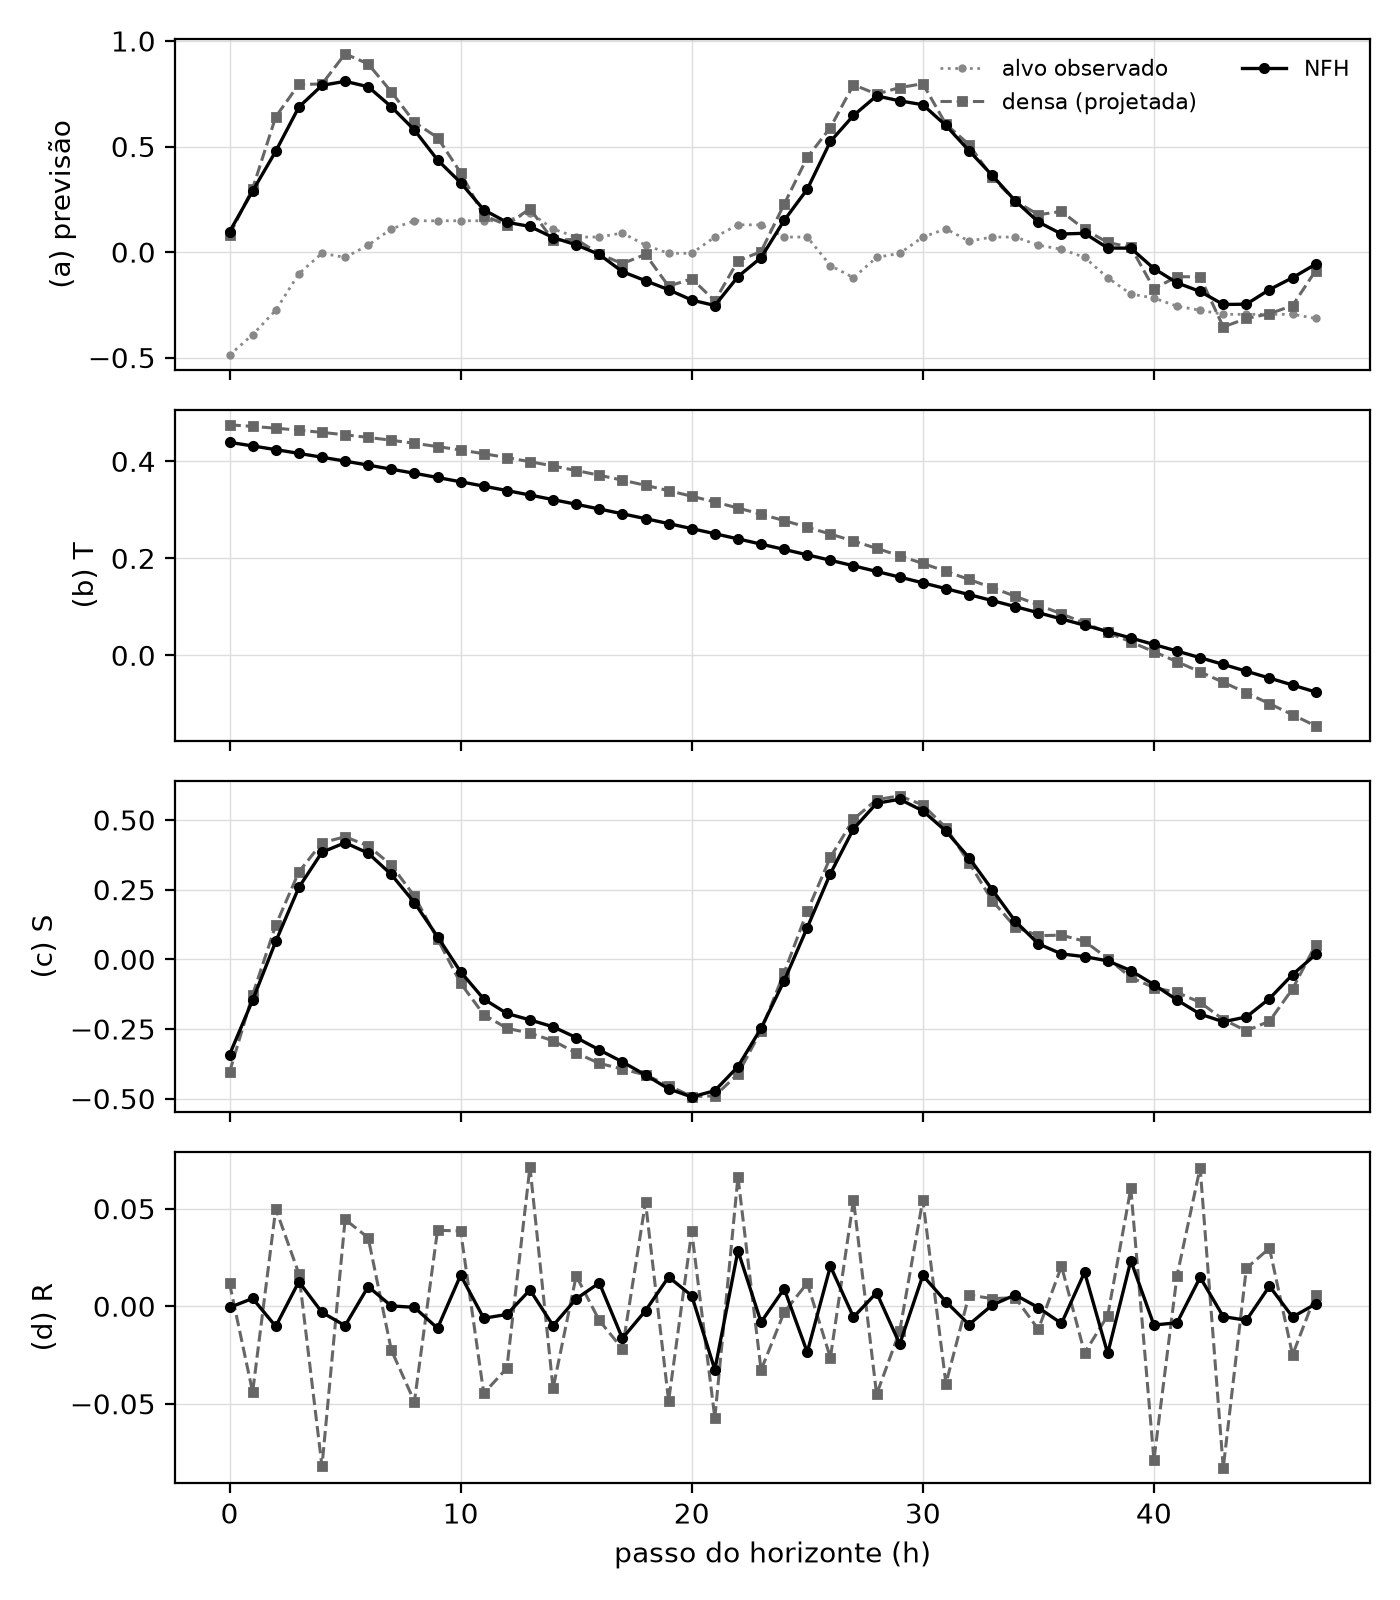
\includegraphics[width=0.95\linewidth]{figuras/expl_ETTh2_U_FreqMLP_w1_f0.25.png}\par\smallskip{\scriptsize Fonte: explicar\_bb.py.}\end{figure}
\subsection{ETTh2\_\allowbreak{}U\_\allowbreak{}iTransformer\_\allowbreak{}w1\_\allowbreak{}f0.\allowbreak{}25}
Semente 10, 2470 janelas de teste. Participações de energia da NFH (mediana [Q1; Q3]): $\varepsilon_T=0,084 [0,030; 0,208]$, $\varepsilon_S=0,916 [0,792; 0,969]$, $\varepsilon_R=0,000 [0,000; 0,000]$. A densa da mesma semente, decomposta só pelo Projetor, dá $\varepsilon_T=0,186 [0,084; 0,335]$, $\varepsilon_S=0,810 [0,661; 0,912]$, $\varepsilon_R=0,003 [0,002; 0,006]$. O harmônico de maior amplitude mediana da NFH é $k=2$ (período 24,0 h, amplitude 0,396). RMSE e MAE de teste desta semente: NFH 0,4770 e 0,3683; densa 0,4882 e 0,3693. IG de $g_T$ (50 janelas, 64 passos, referência zero): maior participação mediana em ``defasagens 1 a 24 h'' (57,0\%); erro de completude mediano 0,000021 (relativo 0,0000). IG de $g_S$ (50 janelas, 64 passos, referência zero): maior participação mediana em ``defasagens 1 a 24 h'' (31,5\%); erro de completude mediano 0,000001 (relativo 0,0000).

\begin{figure}[htbp]\centering\caption{ETTh2\_\allowbreak{}U\_\allowbreak{}iTransformer\_\allowbreak{}w1\_\allowbreak{}f0.\allowbreak{}25: uma janela de teste (previs\~ao, $T$, $S$, $R$ e, nos sint\'eticos, a verdade).}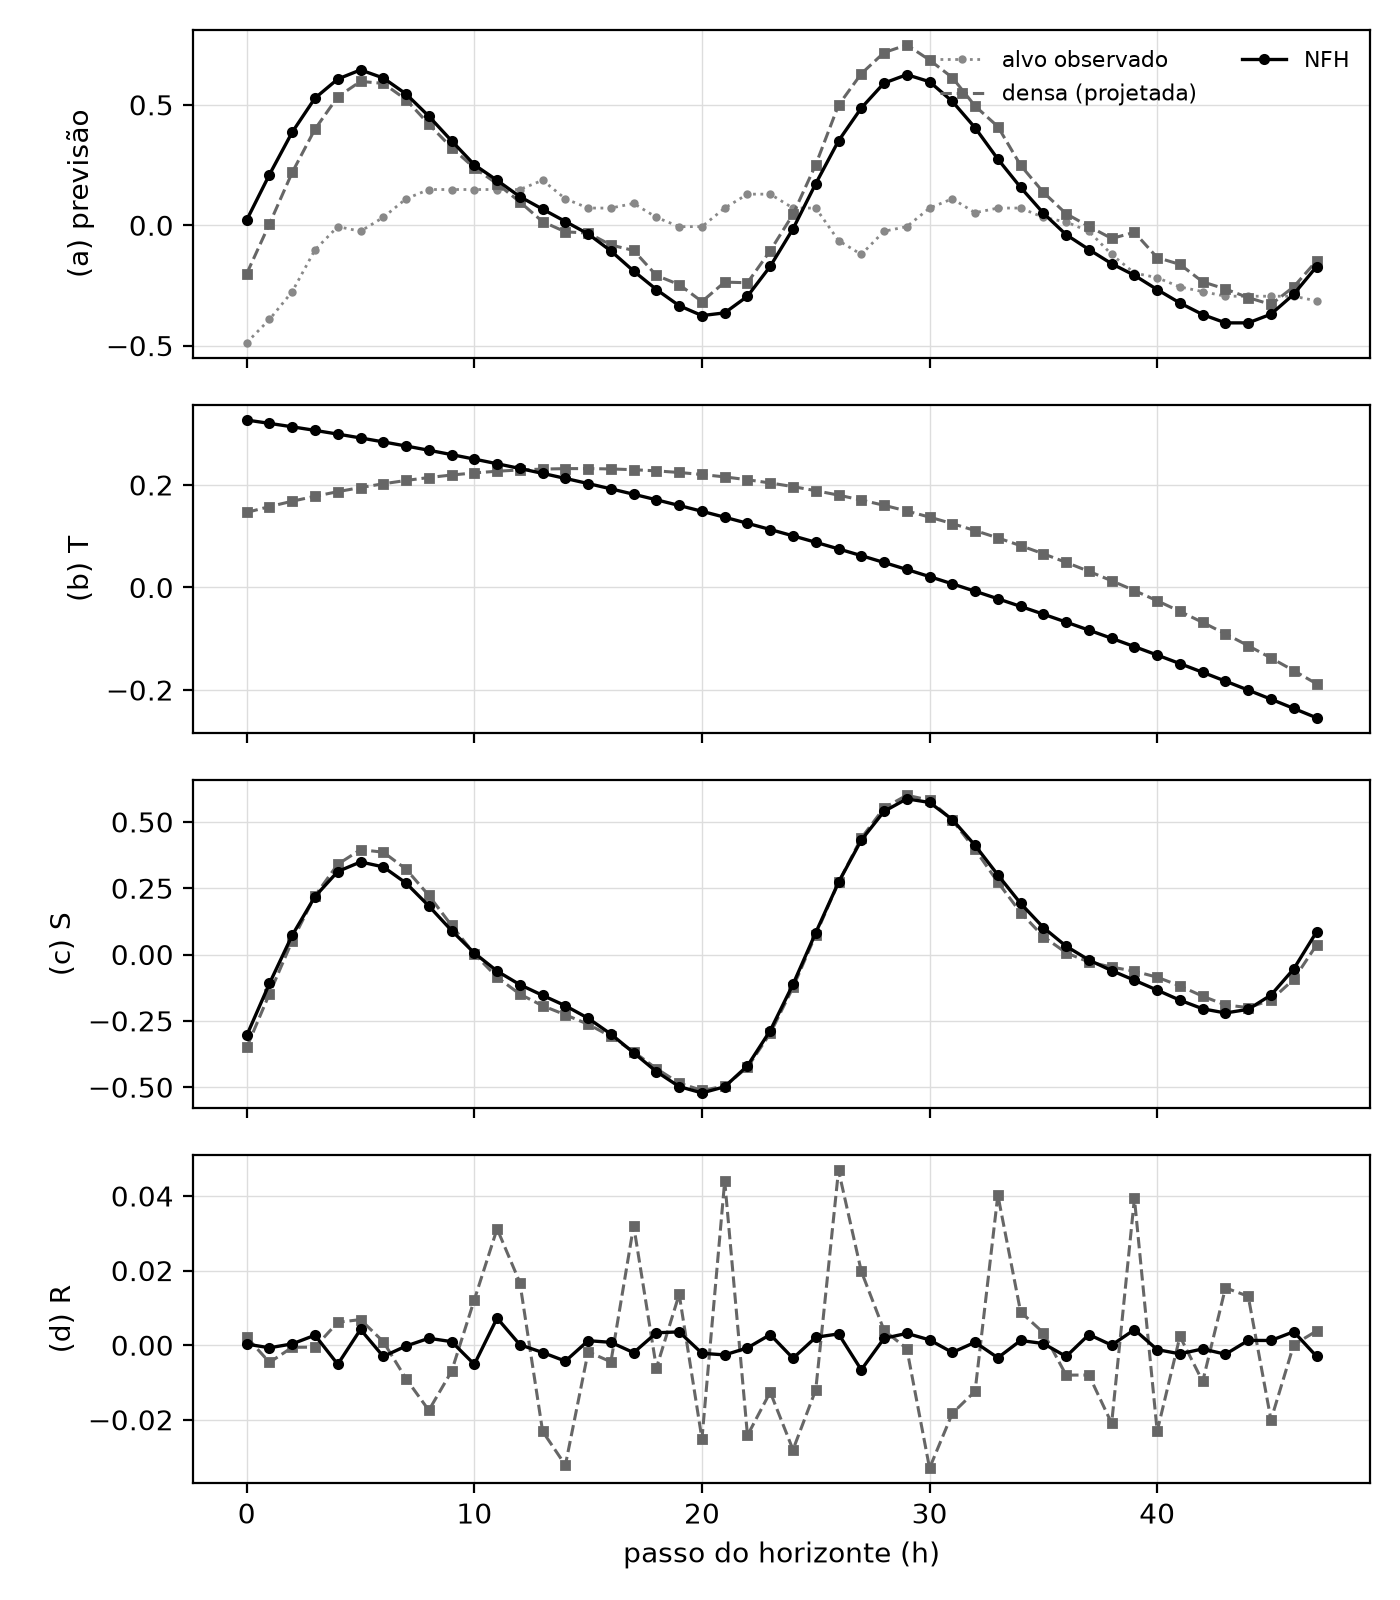
\includegraphics[width=0.95\linewidth]{figuras/expl_ETTh2_U_iTransformer_w1_f0.25.png}\par\smallskip{\scriptsize Fonte: explicar\_bb.py.}\end{figure}
\subsection{SINT-\allowbreak{}M\_\allowbreak{}M\_\allowbreak{}PatchTST\_\allowbreak{}w1\_\allowbreak{}f0.\allowbreak{}1}
Semente 10, 1650 janelas de teste. Participações de energia da NFH (mediana [Q1; Q3]): $\varepsilon_T=0,106 [0,061; 0,178]$, $\varepsilon_S=0,892 [0,820; 0,937]$, $\varepsilon_R=0,001 [0,001; 0,002]$. A densa da mesma semente, decomposta só pelo Projetor, dá $\varepsilon_T=0,111 [0,060; 0,181]$, $\varepsilon_S=0,874 [0,804; 0,924]$, $\varepsilon_R=0,012 [0,008; 0,017]$. O harmônico de maior amplitude mediana da NFH é $k=2$ (período 24,0 h, amplitude 0,814). RMSE e MAE de teste desta semente: NFH 0,2834 e 0,2240; densa 0,3097 e 0,2434. IG de $g_T$ (50 janelas, 64 passos, referência zero): maior participação mediana em ``y'' (100,0\%); erro de completude mediano 0,000003 (relativo 0,0000). IG de $g_S$ (50 janelas, 64 passos, referência zero): maior participação mediana em ``y'' (100,0\%); erro de completude mediano 0,000004 (relativo 0,0000). SINT-M: acerto da tendência (x1) 0,00 com as 5 colunas e 0,58 só com as 4 covariáveis; acerto do ciclo (x2) 0,00 e 0,02. Aviso: aqui $d=5$ e a última coluna é o próprio $y$ passado (na v3, $d=4$); sua participação mediana é 100,0\% em $g_T$ e 100,0\% em $g_S$.

\begin{figure}[htbp]\centering\caption{SINT-\allowbreak{}M\_\allowbreak{}M\_\allowbreak{}PatchTST\_\allowbreak{}w1\_\allowbreak{}f0.\allowbreak{}1: uma janela de teste (previs\~ao, $T$, $S$, $R$ e, nos sint\'eticos, a verdade).}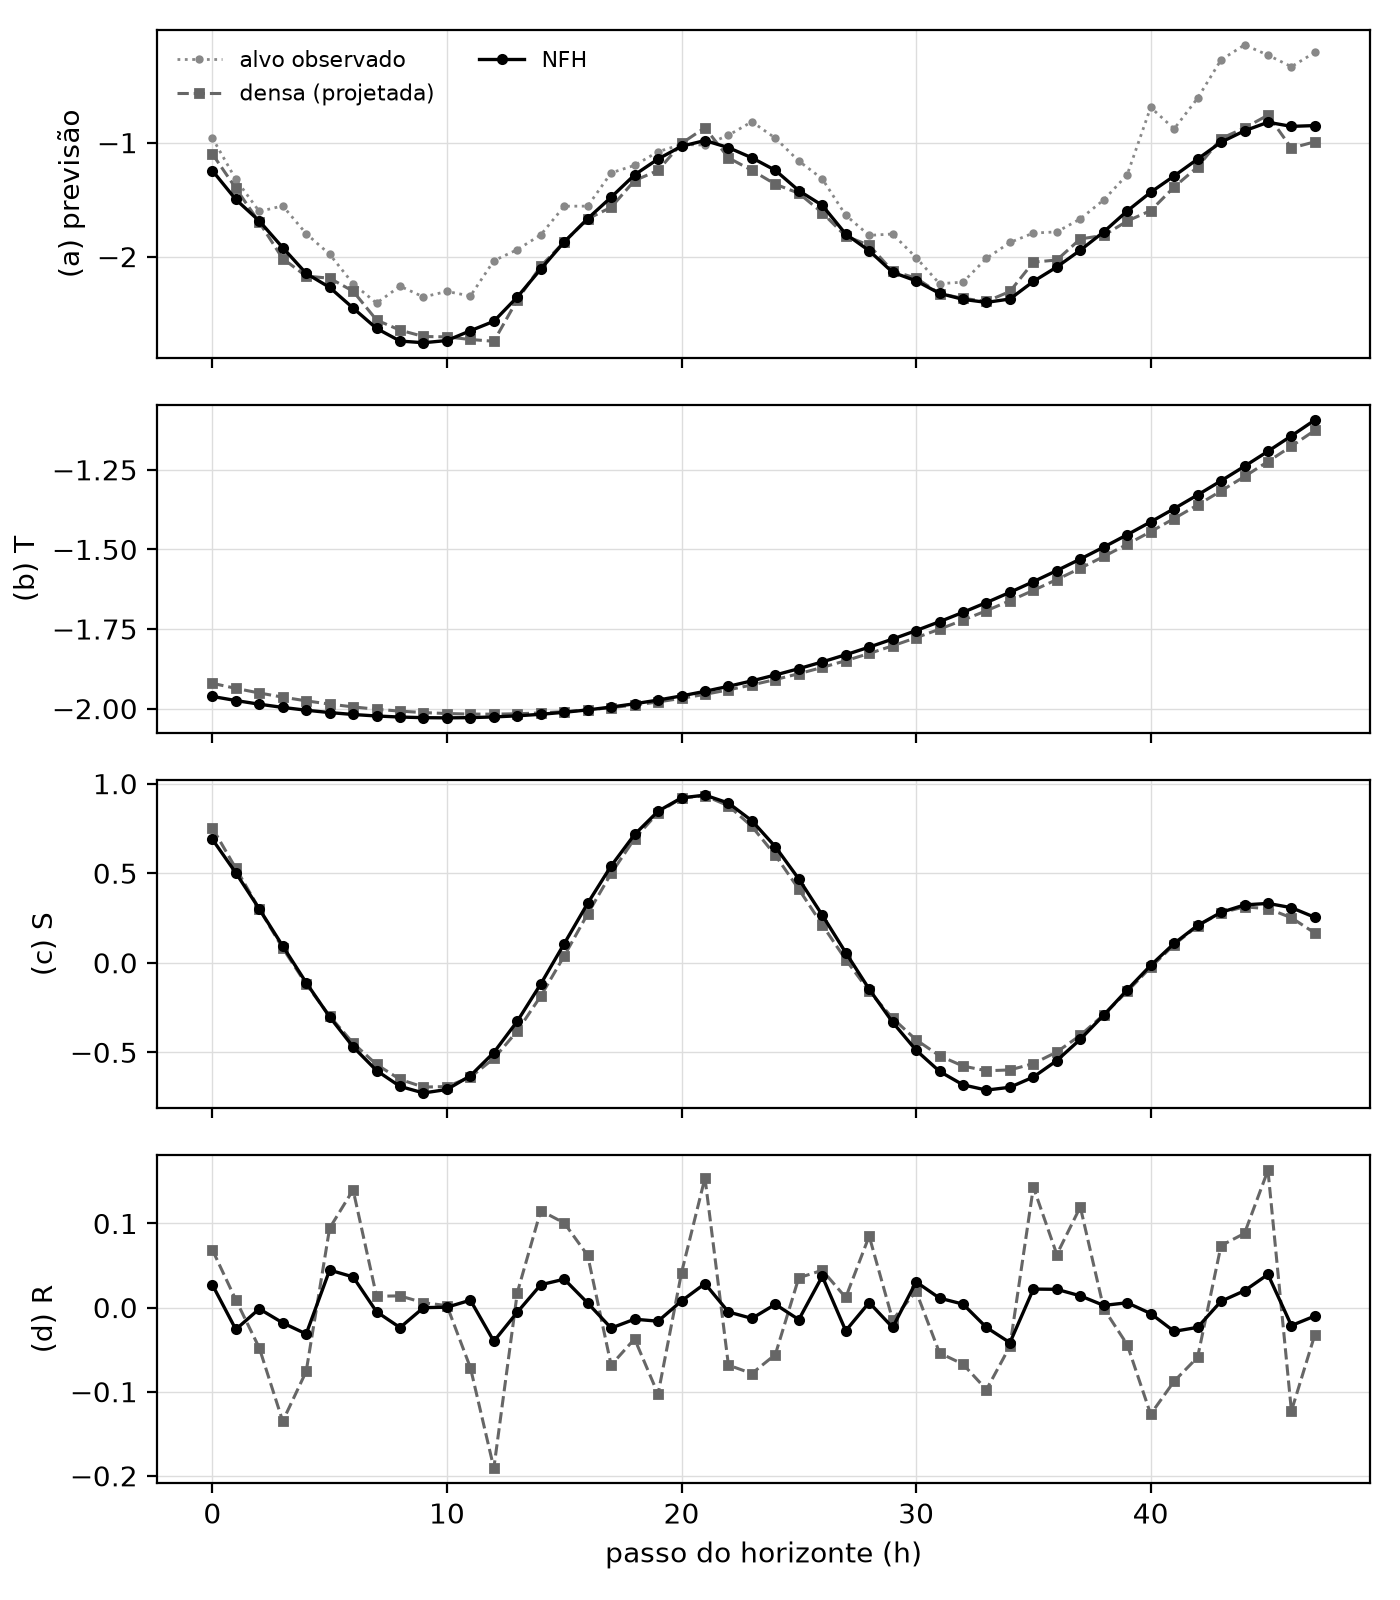
\includegraphics[width=0.95\linewidth]{figuras/expl_SINT-M_M_PatchTST_w1_f0.1.png}\par\smallskip{\scriptsize Fonte: explicar\_bb.py.}\end{figure}
\subsection{SINT-\allowbreak{}M\_\allowbreak{}M\_\allowbreak{}iTransformer\_\allowbreak{}w2\_\allowbreak{}f0.\allowbreak{}25}
Semente 10, 1650 janelas de teste. Participações de energia da NFH (mediana [Q1; Q3]): $\varepsilon_T=0,101 [0,065; 0,167]$, $\varepsilon_S=0,899 [0,833; 0,935]$, $\varepsilon_R=0,000 [0,000; 0,000]$. A densa da mesma semente, decomposta só pelo Projetor, dá $\varepsilon_T=0,111 [0,069; 0,172]$, $\varepsilon_S=0,889 [0,827; 0,929]$, $\varepsilon_R=0,001 [0,001; 0,001]$. O harmônico de maior amplitude mediana da NFH é $k=2$ (período 24,0 h, amplitude 0,899). RMSE e MAE de teste desta semente: NFH 0,2914 e 0,2290; densa 0,3215 e 0,2517. IG de $g_T$ (50 janelas, 64 passos, referência zero): maior participação mediana em ``y'' (100,0\%); erro de completude mediano 0,000007 (relativo 0,0000). IG de $g_S$ (50 janelas, 64 passos, referência zero): maior participação mediana em ``y'' (100,0\%); erro de completude mediano 0,000004 (relativo 0,0000). SINT-M: acerto da tendência (x1) 0,00 com as 5 colunas e 0,46 só com as 4 covariáveis; acerto do ciclo (x2) 0,00 e 0,02. Aviso: aqui $d=5$ e a última coluna é o próprio $y$ passado (na v3, $d=4$); sua participação mediana é 100,0\% em $g_T$ e 100,0\% em $g_S$.

\begin{figure}[htbp]\centering\caption{SINT-\allowbreak{}M\_\allowbreak{}M\_\allowbreak{}iTransformer\_\allowbreak{}w2\_\allowbreak{}f0.\allowbreak{}25: uma janela de teste (previs\~ao, $T$, $S$, $R$ e, nos sint\'eticos, a verdade).}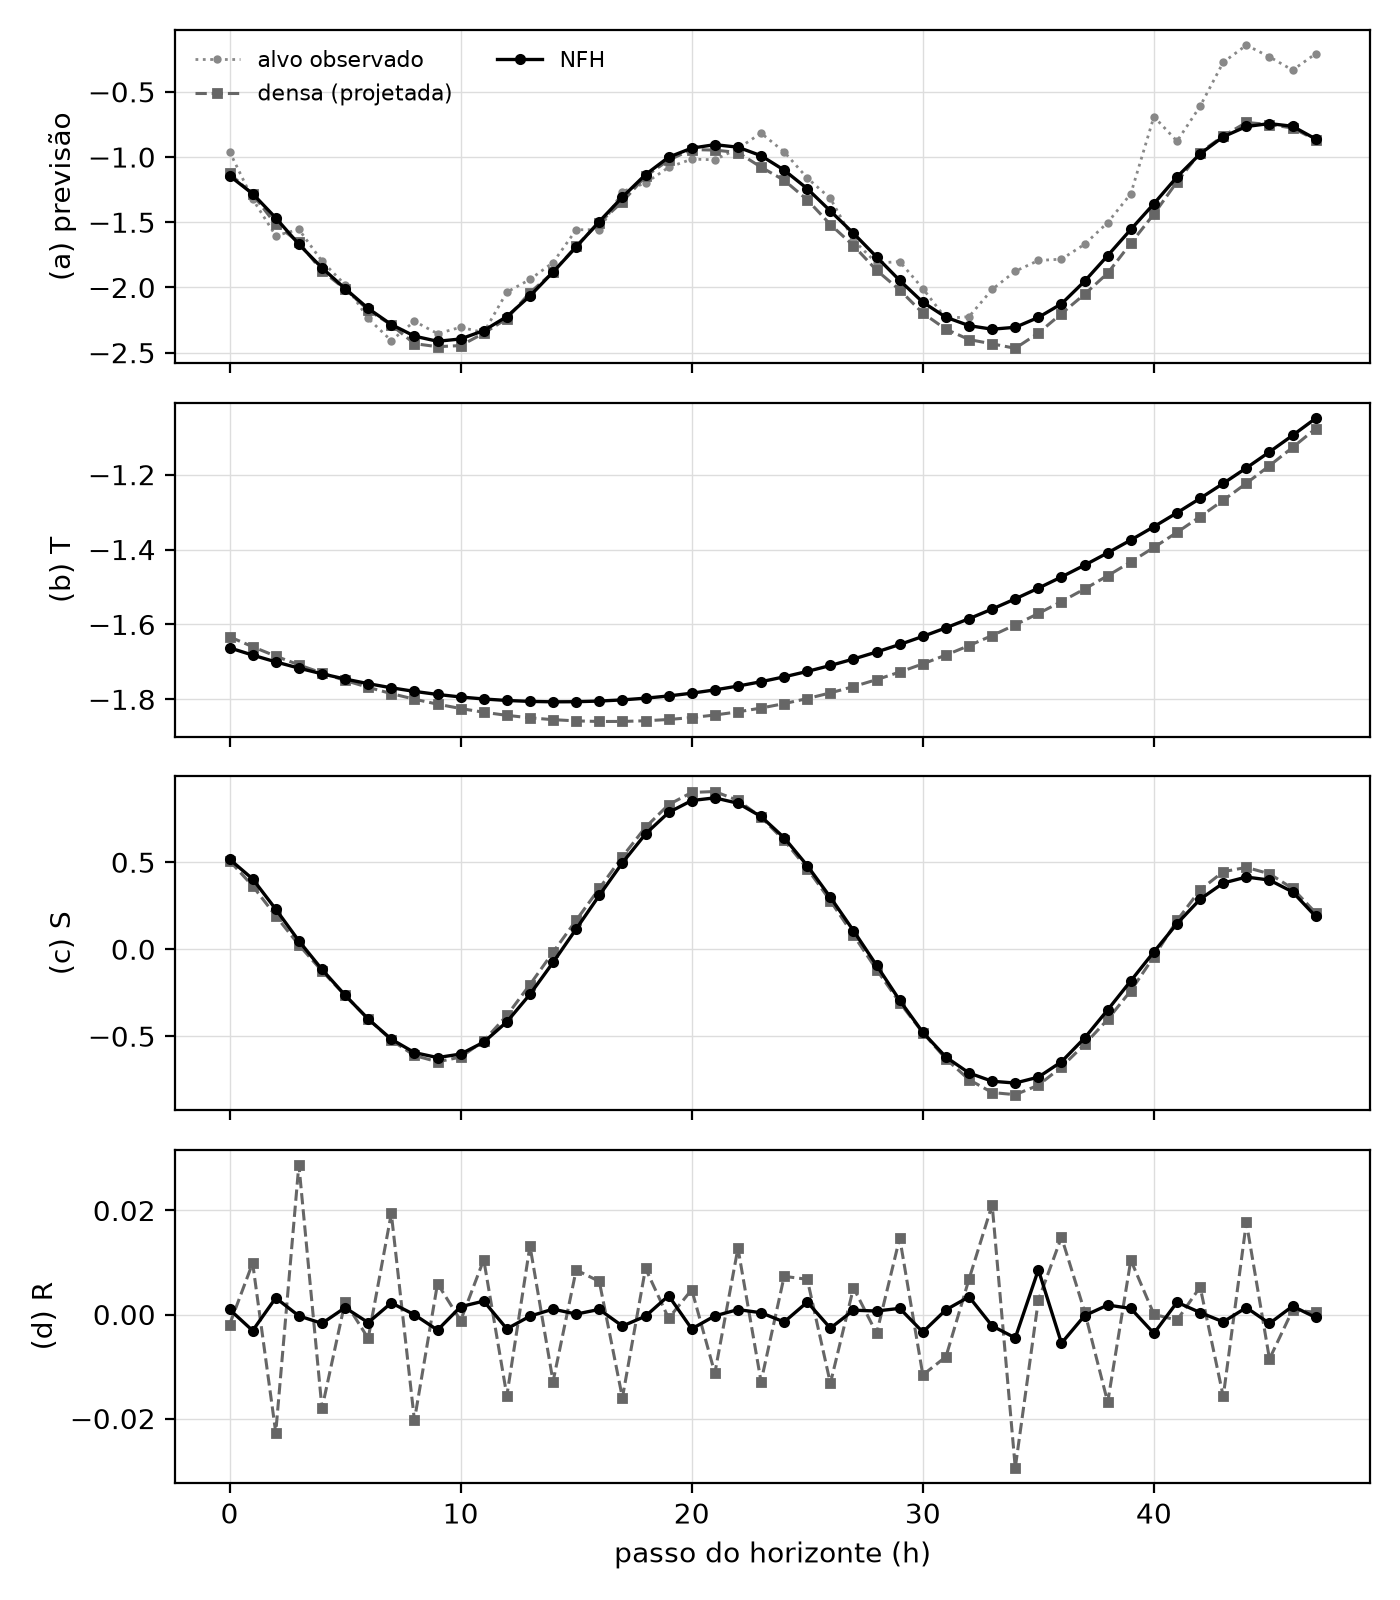
\includegraphics[width=0.95\linewidth]{figuras/expl_SINT-M_M_iTransformer_w2_f0.25.png}\par\smallskip{\scriptsize Fonte: explicar\_bb.py.}\end{figure}
\subsection{SINT-\allowbreak{}U48\_\allowbreak{}U\_\allowbreak{}DLinear\_\allowbreak{}w1\_\allowbreak{}f0.\allowbreak{}1}
Semente 10, 1657 janelas de teste. Participações de energia da NFH (mediana [Q1; Q3]): $\varepsilon_T=0,068 [0,048; 0,107]$, $\varepsilon_S=0,932 [0,893; 0,952]$, $\varepsilon_R=0,000 [0,000; 0,000]$. A densa da mesma semente, decomposta só pelo Projetor, dá $\varepsilon_T=0,076 [0,054; 0,114]$, $\varepsilon_S=0,914 [0,875; 0,937]$, $\varepsilon_R=0,009 [0,007; 0,013]$. O harmônico de maior amplitude mediana da NFH é $k=2$ (período 24,0 h, amplitude 0,820). RMSE e MAE de teste desta semente: NFH 0,3062 e 0,2433; densa 0,3140 e 0,2490. IG de $g_T$ (50 janelas, 64 passos, referência zero): maior participação mediana em ``defasagens 1 a 24 h'' (56,0\%); erro de completude mediano 0,000000 (relativo 0,0000). IG de $g_S$ (50 janelas, 64 passos, referência zero): maior participação mediana em ``defasagens 25 a 48 h'' (32,9\%); erro de completude mediano 0,000002 (relativo 0,0000). SINT-U48, contra o sinal sem ruído do futuro decomposto pelas mesmas fórmulas: RMSE da previsão da NFH contra o sinal 0,1500 (densa projetada 0,1652); RMSE de $T$ 0,1199 e de $S$ 0,0900; erro relativo mediano de $S$ 0,134. Referência amostral do oráculo (janelas de teste): 0,2671.

\begin{figure}[htbp]\centering\caption{SINT-\allowbreak{}U48\_\allowbreak{}U\_\allowbreak{}DLinear\_\allowbreak{}w1\_\allowbreak{}f0.\allowbreak{}1: uma janela de teste (previs\~ao, $T$, $S$, $R$ e, nos sint\'eticos, a verdade).}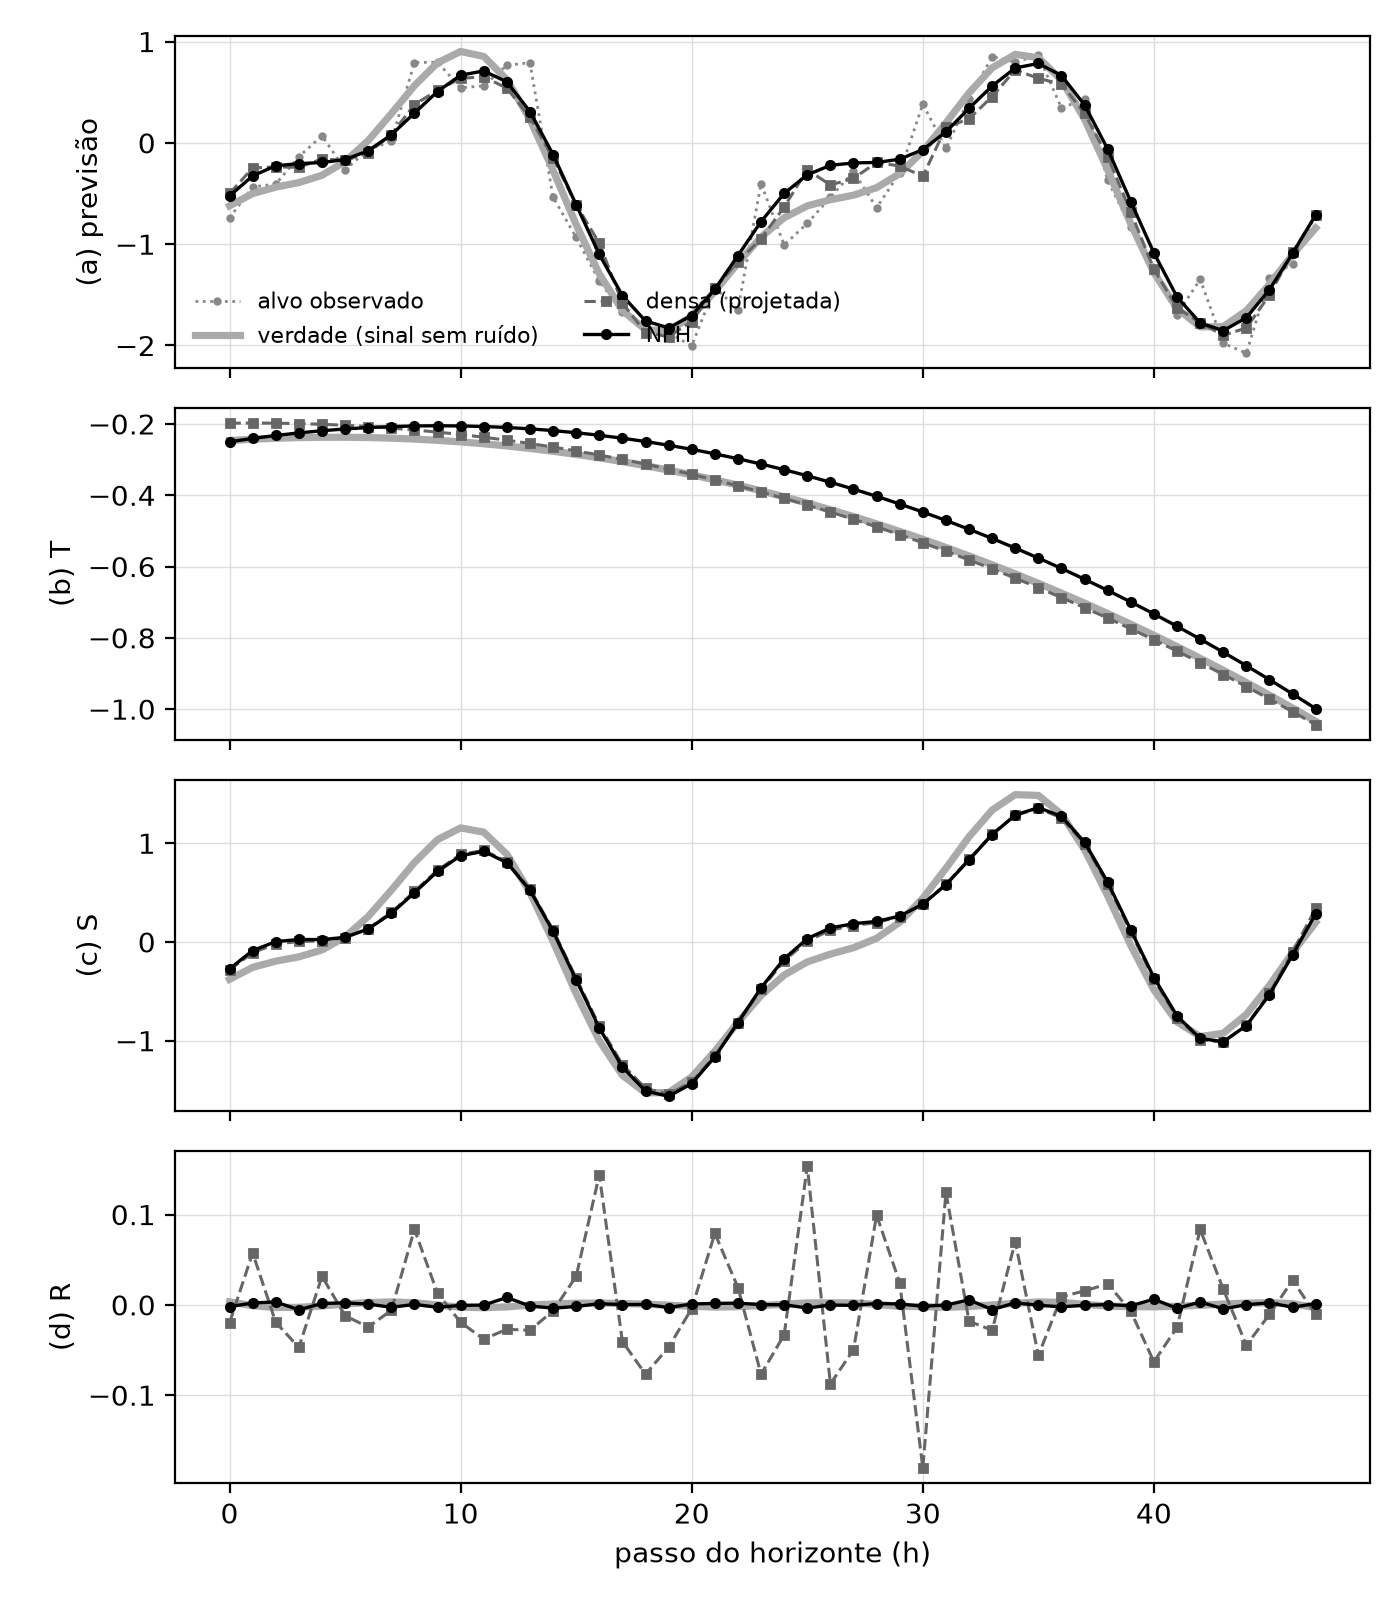
\includegraphics[width=0.95\linewidth]{figuras/expl_SINT-U48_U_DLinear_w1_f0.1.png}\par\smallskip{\scriptsize Fonte: explicar\_bb.py.}\end{figure}
\subsection{SINT-\allowbreak{}U48\_\allowbreak{}U\_\allowbreak{}Linear\_\allowbreak{}w1\_\allowbreak{}f0.\allowbreak{}1}
Semente 10, 1657 janelas de teste. Participações de energia da NFH (mediana [Q1; Q3]): $\varepsilon_T=0,074 [0,049; 0,114]$, $\varepsilon_S=0,926 [0,886; 0,951]$, $\varepsilon_R=0,000 [0,000; 0,000]$. A densa da mesma semente, decomposta só pelo Projetor, dá $\varepsilon_T=0,076 [0,053; 0,119]$, $\varepsilon_S=0,911 [0,866; 0,935]$, $\varepsilon_R=0,012 [0,009; 0,017]$. O harmônico de maior amplitude mediana da NFH é $k=2$ (período 24,0 h, amplitude 0,814). RMSE e MAE de teste desta semente: NFH 0,3066 e 0,2436; densa 0,3152 e 0,2499. IG de $g_T$ (50 janelas, 64 passos, referência zero): maior participação mediana em ``defasagens 1 a 24 h'' (55,3\%); erro de completude mediano 0,000000 (relativo 0,0000). IG de $g_S$ (50 janelas, 64 passos, referência zero): maior participação mediana em ``defasagens 25 a 48 h'' (33,1\%); erro de completude mediano 0,000002 (relativo 0,0000). SINT-U48, contra o sinal sem ruído do futuro decomposto pelas mesmas fórmulas: RMSE da previsão da NFH contra o sinal 0,1507 (densa projetada 0,1680); RMSE de $T$ 0,1204 e de $S$ 0,0906; erro relativo mediano de $S$ 0,135. Referência amostral do oráculo (janelas de teste): 0,2671.

\begin{figure}[htbp]\centering\caption{SINT-\allowbreak{}U48\_\allowbreak{}U\_\allowbreak{}Linear\_\allowbreak{}w1\_\allowbreak{}f0.\allowbreak{}1: uma janela de teste (previs\~ao, $T$, $S$, $R$ e, nos sint\'eticos, a verdade).}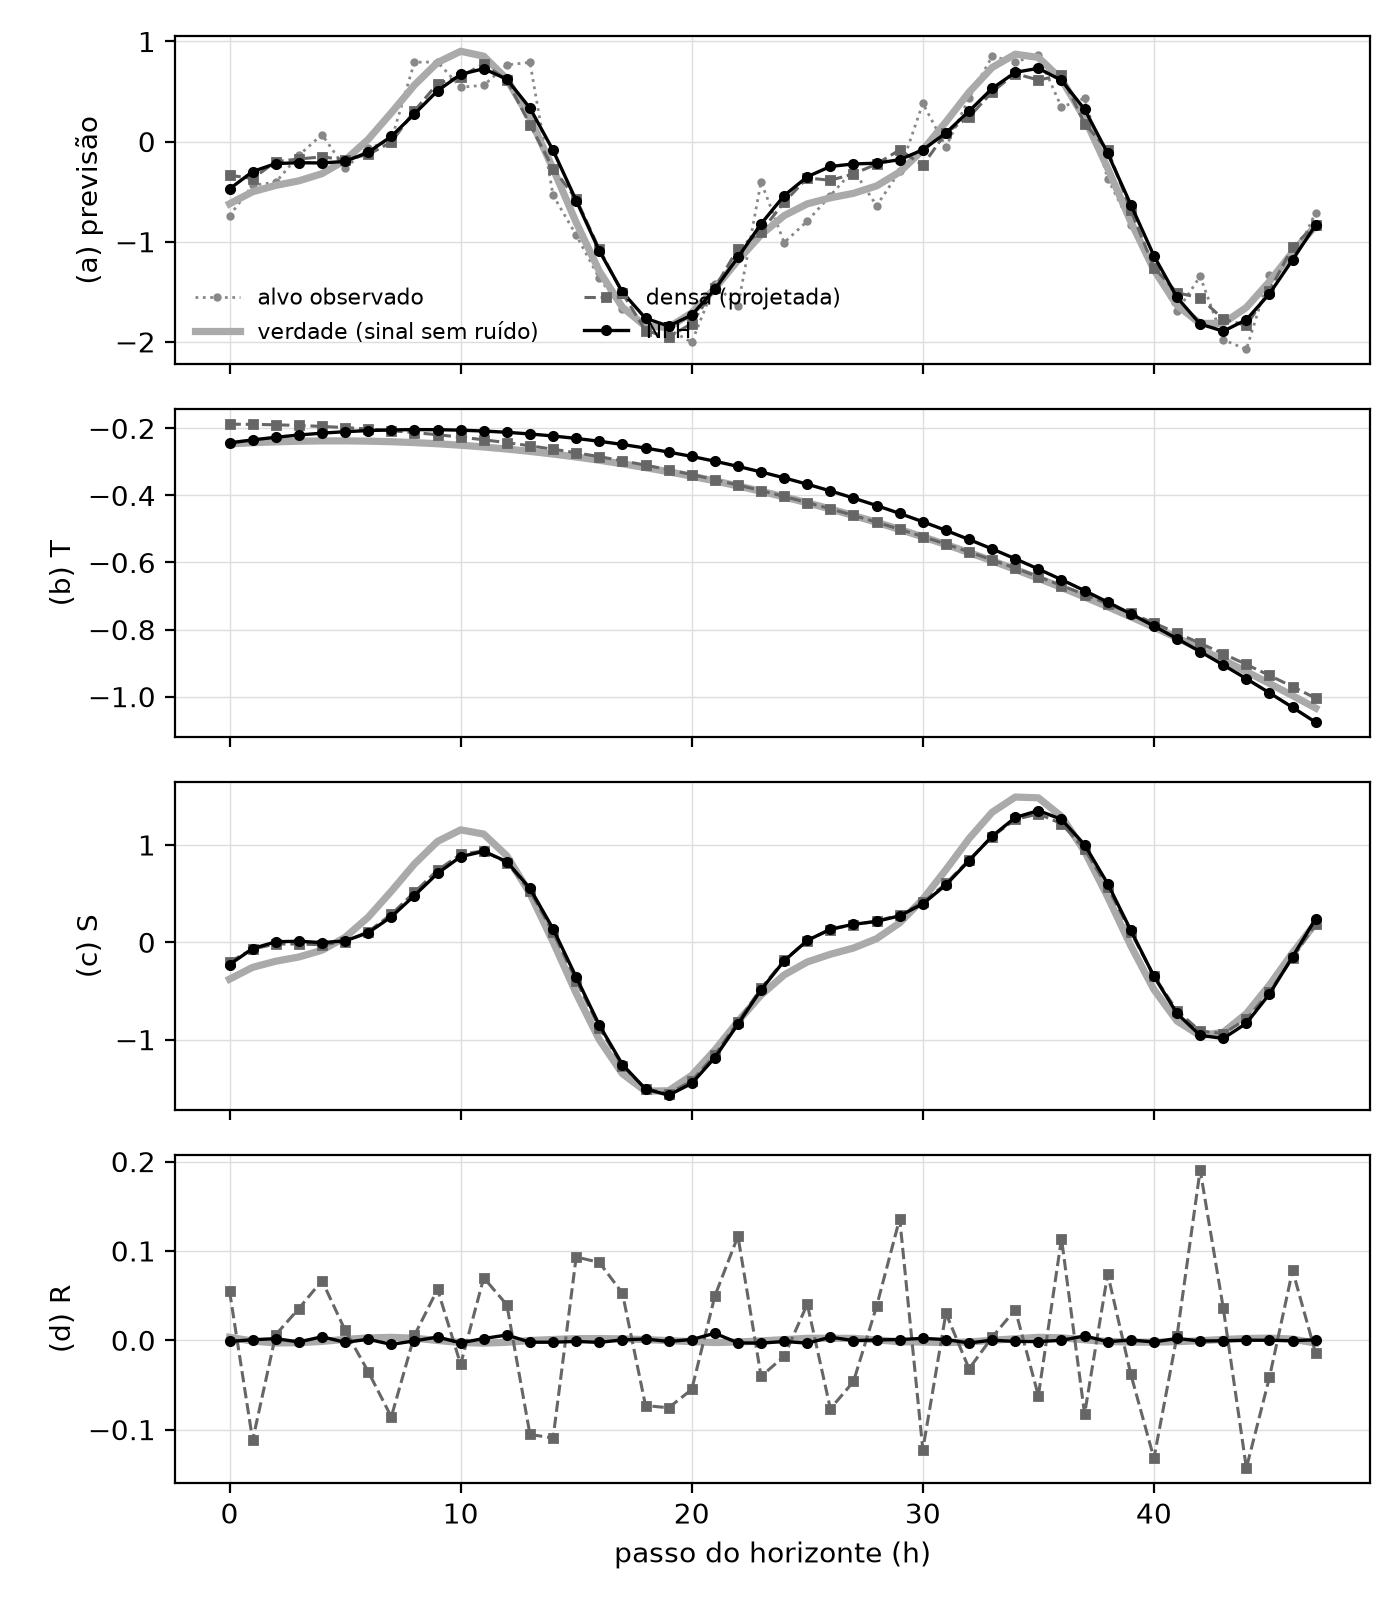
\includegraphics[width=0.95\linewidth]{figuras/expl_SINT-U48_U_Linear_w1_f0.1.png}\par\smallskip{\scriptsize Fonte: explicar\_bb.py.}\end{figure}
\appendix
\section{Todas as combinações da T1}\label{ap:t1}
\tiny
\setlength{\tabcolsep}{2pt}
\begin{longtable}{llrlrrrrrrll}
\caption{T1: todas as combina\c{c}\~oes (melhor variante NFH pelo RMSE de valida\c{c}\~ao; diferen\c{c}as contra a densa+E, e contra a densa nas colunas ``vs densa'').}\label{tab:t1_todas}\\
\toprule
Conjunto & Backbone & Fr. & Variante & \shortstack[l]{RMSE val} & \shortstack[l]{MAE val} & \shortstack[l]{RMSE teste} & \shortstack[l]{MAE teste} & \shortstack[l]{RMSE teste\\ vs densa} & \shortstack[l]{MAE teste\\ vs densa} & Qualif. & T2 \\ \midrule
\endfirsthead
\toprule
Conjunto & Backbone & Fr. & Variante & \shortstack[l]{RMSE val} & \shortstack[l]{MAE val} & \shortstack[l]{RMSE teste} & \shortstack[l]{MAE teste} & \shortstack[l]{RMSE teste\\ vs densa} & \shortstack[l]{MAE teste\\ vs densa} & Qualif. & T2 \\ \midrule
\endhead
\bottomrule
\multicolumn{12}{l}{\textit{Fonte: resultados/t1.csv e selecao\_T1.md.}}\\
\endlastfoot
ETTh1-M & PatchTST & 0.25 & \texttt{zero\_\allowbreak{}L1000\_\allowbreak{}K10} & \textminus{}8,84\% & \textminus{}7,16\% & \textminus{}3,60\% & \textminus{}0,40\% & \textminus{}4,66\% & \textminus{}1,86\% & sim & sim \\
SINT-M-M & PatchTST & 0.1 & \texttt{zero\_\allowbreak{}L1000\_\allowbreak{}K10} & \textminus{}8,20\% & \textminus{}7,51\% & \textminus{}5,48\% & \textminus{}5,94\% & \textminus{}10,28\% & \textminus{}10,46\% & sim & sim \\
SINT-M-M & Conv1D+LSTM & 1 & \texttt{zero\_\allowbreak{}L100\_\allowbreak{}K10} & \textminus{}6,14\% & \textminus{}7,26\% & \textminus{}1,89\% & \textminus{}1,75\% & \textminus{}1,89\% & \textminus{}1,75\% & sim & sim \\
SINT-M-M & iTransformer & 0.25 & \texttt{zero\_\allowbreak{}L100\_\allowbreak{}K10} & \textminus{}5,83\% & \textminus{}6,44\% & \textminus{}7,68\% & \textminus{}9,25\% & \textminus{}7,68\% & \textminus{}9,25\% & sim & sim \\
SINT-M-M & iTransformer & 0.1 & \texttt{zero\_\allowbreak{}L1000\_\allowbreak{}K4} & \textminus{}5,63\% & \textminus{}4,87\% & \textminus{}3,69\% & \textminus{}2,41\% & \textminus{}5,52\% & \textminus{}4,77\% & sim & n\~ao \\
ETTh1-M & iTransformer & 0.25 & \texttt{zero\_\allowbreak{}L1000\_\allowbreak{}K10} & \textminus{}5,03\% & \textminus{}5,09\% & +3,20\% & +5,58\% & +6,87\% & +7,92\% & sim & sim \\
air\_quality-U & PatchTST & 1 & \texttt{zero\_\allowbreak{}L1000\_\allowbreak{}K10} & \textminus{}5,02\% & \textminus{}5,29\% & +1,52\% & \textminus{}0,42\% & \textminus{}1,85\% & \textminus{}3,11\% & sim & sim \\
ETTh1-U & PatchTST & 0.25 & \texttt{conv\_\allowbreak{}L1000\_\allowbreak{}K10} & \textminus{}4,76\% & \textminus{}4,25\% & \textminus{}7,24\% & \textminus{}5,55\% & \textminus{}3,97\% & \textminus{}3,85\% & sim & n\~ao \\
seoul\_bike-U & PatchTST & 0.25 & \texttt{zero\_\allowbreak{}L1000\_\allowbreak{}K10} & \textminus{}4,09\% & \textminus{}2,71\% & \textminus{}1,86\% & \textminus{}0,49\% & \textminus{}4,88\% & \textminus{}5,47\% & sim & n\~ao \\
ETTh2-U & iTransformer & 0.25 & \texttt{zero\_\allowbreak{}L1000\_\allowbreak{}K10} & \textminus{}3,66\% & \textminus{}3,48\% & \textminus{}2,55\% & \textminus{}2,91\% & \textminus{}2,06\% & \textminus{}2,18\% & sim & sim \\
SINT-M-M & Conv1D+LSTM & 0.25 & \texttt{zero\_\allowbreak{}L100\_\allowbreak{}K10} & \textminus{}3,03\% & \textminus{}4,00\% & \textminus{}6,29\% & \textminus{}6,32\% & \textminus{}4,66\% & \textminus{}4,60\% & sim & n\~ao \\
ETTh2-U & PatchTST & 0.25 & \texttt{conv\_\allowbreak{}L1000\_\allowbreak{}K10} & \textminus{}2,85\% & \textminus{}3,09\% & \textminus{}0,40\% & +2,35\% & \textminus{}0,40\% & +2,35\% & sim & n\~ao \\
SINT-M-M & TSMixer & 0.1 & \texttt{conv\_\allowbreak{}L1000\_\allowbreak{}K10} & \textminus{}2,77\% & \textminus{}1,91\% & \textminus{}2,62\% & \textminus{}3,33\% & \textminus{}2,73\% & \textminus{}3,03\% & sim & n\~ao \\
SINT-M-M & MLP & 0.25 & \texttt{conv\_\allowbreak{}L1000\_\allowbreak{}K10} & \textminus{}2,68\% & \textminus{}2,03\% & \textminus{}0,21\% & \textminus{}0,25\% & \textminus{}9,83\% & \textminus{}9,61\% & sim & n\~ao \\
SINT-U48-U & Linear & 0.1 & \texttt{zero\_\allowbreak{}L1000\_\allowbreak{}K4} & \textminus{}2,37\% & \textminus{}2,35\% & \textminus{}2,46\% & \textminus{}2,22\% & \textminus{}2,78\% & \textminus{}2,59\% & sim & sim \\
SINT-U48-U & PatchTST & 0.1 & \texttt{zero\_\allowbreak{}L1000\_\allowbreak{}K4} & \textminus{}2,27\% & \textminus{}2,02\% & \textminus{}4,86\% & \textminus{}4,95\% & \textminus{}7,76\% & \textminus{}7,96\% & sim & n\~ao \\
SINT-M-M & FreqMLP & 0.1 & \texttt{zero\_\allowbreak{}L1000\_\allowbreak{}K10} & \textminus{}2,25\% & \textminus{}0,27\% & +11,32\% & +10,52\% & +11,32\% & +10,52\% & sim & n\~ao \\
SINT-U48-U & DLinear & 0.1 & \texttt{zero\_\allowbreak{}L1000\_\allowbreak{}K4} & \textminus{}2,14\% & \textminus{}2,18\% & \textminus{}2,22\% & \textminus{}2,05\% & \textminus{}2,51\% & \textminus{}2,33\% & sim & sim \\
ETTh2-U & FreqMLP & 0.25 & \texttt{conv\_\allowbreak{}L1000\_\allowbreak{}K10} & \textminus{}2,04\% & \textminus{}1,86\% & \textminus{}2,26\% & \textminus{}1,30\% & \textminus{}2,26\% & \textminus{}1,30\% & sim & sim \\
air\_quality-U & iTransformer & 1 & \texttt{conv\_\allowbreak{}L1000\_\allowbreak{}K10} & \textminus{}1,94\% & \textminus{}0,15\% & +1,53\% & +1,79\% & \textminus{}3,12\% & \textminus{}1,85\% & sim & n\~ao \\
SINT-U48-U & PatchTST & 0.25 & \texttt{conv\_\allowbreak{}L1000\_\allowbreak{}K10} & \textminus{}1,92\% & \textminus{}2,17\% & \textminus{}1,93\% & \textminus{}2,16\% & \textminus{}2,16\% & \textminus{}2,15\% & sim & n\~ao \\
ETTh1-U & iTransformer & 0.25 & \texttt{conv\_\allowbreak{}L1000\_\allowbreak{}K10} & \textminus{}1,92\% & \textminus{}2,37\% & +0,71\% & +0,99\% & \textminus{}2,52\% & \textminus{}4,76\% & sim & n\~ao \\
SINT-M-M & FreqMLP & 0.25 & \texttt{zero\_\allowbreak{}L100\_\allowbreak{}K10} & \textminus{}1,92\% & \textminus{}0,76\% & +4,34\% & +4,59\% & +4,34\% & +4,59\% & sim & n\~ao \\
SINT-U48-U & iTransformer & 0.25 & \texttt{zero\_\allowbreak{}L1000\_\allowbreak{}K10} & \textminus{}1,91\% & \textminus{}1,67\% & \textminus{}0,10\% & \textminus{}0,49\% & \textminus{}0,96\% & \textminus{}1,29\% & sim & n\~ao \\
SINT-U48-U & FreqMLP & 0.1 & \texttt{zero\_\allowbreak{}L100\_\allowbreak{}K10} & \textminus{}1,86\% & \textminus{}1,60\% & \textminus{}0,61\% & \textminus{}0,87\% & \textminus{}1,22\% & \textminus{}1,42\% & sim & sim \\
SINT-M-M & MLP & 1 & \texttt{conv\_\allowbreak{}L1000\_\allowbreak{}K10} & \textminus{}1,76\% & \textminus{}0,94\% & \textminus{}5,29\% & \textminus{}5,24\% & \textminus{}8,37\% & \textminus{}8,53\% & sim & n\~ao \\
air\_quality-U & PatchTST & 0.25 & \texttt{zero\_\allowbreak{}L100\_\allowbreak{}K10} & \textminus{}1,73\% & \textminus{}2,54\% & +2,91\% & +2,33\% & +2,91\% & +2,33\% & sim & n\~ao \\
seoul\_bike-U & Conv1D+LSTM & 1 & \texttt{conv\_\allowbreak{}L1000\_\allowbreak{}K10} & \textminus{}1,73\% & \textminus{}2,28\% & +0,41\% & \textminus{}0,93\% & +0,41\% & \textminus{}0,93\% & sim & sim \\
SINT-M-M & Conv1D+LSTM & 0.1 & \texttt{conv\_\allowbreak{}L1000\_\allowbreak{}K10} & \textminus{}1,71\% & \textminus{}0,68\% & \textminus{}3,44\% & \textminus{}3,09\% & \textminus{}2,27\% & \textminus{}2,21\% & sim & n\~ao \\
jena\_climate-U & iTransformer & 0.25 & \texttt{conv\_\allowbreak{}L1000\_\allowbreak{}K10} & \textminus{}1,70\% & \textminus{}2,17\% & \textminus{}1,90\% & \textminus{}2,84\% & \textminus{}1,90\% & \textminus{}2,84\% & sim & n\~ao \\
ETTh2-U & PatchTST & 1 & \texttt{zero\_\allowbreak{}L100\_\allowbreak{}K10} & \textminus{}1,62\% & \textminus{}1,95\% & \textminus{}1,51\% & \textminus{}0,97\% & \textminus{}1,51\% & \textminus{}0,97\% & sim & n\~ao \\
seoul\_bike-U & PatchTST & 1 & \texttt{zero\_\allowbreak{}L100\_\allowbreak{}K10} & \textminus{}1,46\% & \textminus{}1,29\% & +1,19\% & +0,54\% & +1,19\% & +0,54\% & sim & n\~ao \\
SINT-U48-U & FreqMLP & 0.25 & \texttt{zero\_\allowbreak{}L100\_\allowbreak{}K10} & \textminus{}1,41\% & \textminus{}1,38\% & +0,52\% & +0,29\% & +0,09\% & \textminus{}0,08\% & sim & n\~ao \\
SINT-U48-U & iTransformer & 0.1 & \texttt{zero\_\allowbreak{}L100\_\allowbreak{}K10} & \textminus{}1,36\% & \textminus{}1,46\% & \textminus{}1,50\% & \textminus{}1,75\% & \textminus{}2,91\% & \textminus{}3,28\% & sim & n\~ao \\
SINT-U48-U & TSMixer & 0.1 & \texttt{zero\_\allowbreak{}L100\_\allowbreak{}K10} & \textminus{}1,33\% & \textminus{}1,18\% & \textminus{}1,38\% & \textminus{}1,34\% & \textminus{}1,74\% & \textminus{}1,70\% & sim & n\~ao \\
ETTh1-U & TSMixer & 0.25 & \texttt{conv\_\allowbreak{}L1000\_\allowbreak{}K10} & \textminus{}1,30\% & \textminus{}1,16\% & +2,50\% & +5,49\% & +2,53\% & +4,74\% & sim & n\~ao \\
ETTh1-U & Conv1D+LSTM & 0.25 & \texttt{conv\_\allowbreak{}L1000\_\allowbreak{}K10} & \textminus{}1,29\% & \textminus{}1,58\% & \textminus{}1,07\% & \textminus{}0,94\% & \textminus{}1,07\% & \textminus{}0,94\% & sim & n\~ao \\
SINT-U48-U & iTransformer & 1 & \texttt{zero\_\allowbreak{}L1000\_\allowbreak{}K4} & \textminus{}1,25\% & \textminus{}1,18\% & +0,62\% & +0,41\% & +0,04\% & \textminus{}0,39\% & sim & n\~ao \\
jena\_climate-U & PatchTST & 0.25 & \texttt{conv\_\allowbreak{}L1000\_\allowbreak{}K10} & \textminus{}1,25\% & \textminus{}1,08\% & \textminus{}2,13\% & \textminus{}1,98\% & \textminus{}5,21\% & \textminus{}5,85\% & sim & n\~ao \\
ETTh1-M & TSMixer & 0.25 & \texttt{conv\_\allowbreak{}L1000\_\allowbreak{}K10} & \textminus{}1,23\% & \textminus{}0,51\% & +2,05\% & +4,62\% & +2,17\% & +4,68\% & sim & n\~ao \\
SINT-U48-U & Linear & 0.25 & \texttt{zero\_\allowbreak{}L1000\_\allowbreak{}K4} & \textminus{}1,22\% & \textminus{}1,01\% & \textminus{}1,55\% & \textminus{}1,37\% & \textminus{}2,06\% & \textminus{}1,90\% & sim & n\~ao \\
SINT-M-M & LSTM & 0.1 & \texttt{conv\_\allowbreak{}L1000\_\allowbreak{}K10} & \textminus{}1,12\% & \textminus{}0,22\% & \textminus{}5,83\% & \textminus{}6,27\% & \textminus{}2,82\% & \textminus{}3,76\% & sim & n\~ao \\
ETTh2-U & iTransformer & 1 & \texttt{zero\_\allowbreak{}L1000\_\allowbreak{}K10} & \textminus{}1,12\% & \textminus{}1,12\% & +0,19\% & +0,42\% & +0,19\% & +0,42\% & sim & n\~ao \\
SINT-U48-U & LSTM & 0.25 & \texttt{zero\_\allowbreak{}L100\_\allowbreak{}K10} & \textminus{}1,12\% & \textminus{}0,93\% & +2,69\% & +2,64\% & +1,33\% & +1,30\% & sim & n\~ao \\
melbourne\_pedestrian\_southbank-U & LSTM & 0.25 & \texttt{conv\_\allowbreak{}L1000\_\allowbreak{}K10} & \textminus{}1,09\% & \textminus{}0,23\% & \textminus{}1,21\% & \textminus{}0,30\% & \textminus{}0,58\% & +0,56\% & sim & n\~ao \\
SINT-U48-U & TSMixer & 0.25 & \texttt{zero\_\allowbreak{}L100\_\allowbreak{}K10} & \textminus{}1,09\% & \textminus{}1,11\% & \textminus{}1,59\% & \textminus{}1,77\% & \textminus{}2,19\% & \textminus{}2,39\% & sim & n\~ao \\
SINT-M-M & PatchTST & 0.25 & \texttt{zero\_\allowbreak{}L100\_\allowbreak{}K10} & \textminus{}1,06\% & \textminus{}1,17\% & \textminus{}5,40\% & \textminus{}6,13\% & \textminus{}5,40\% & \textminus{}6,13\% & sim & n\~ao \\
SINT-M-M & iTransformer & 1 & \texttt{zero\_\allowbreak{}L1000\_\allowbreak{}K10} & \textminus{}1,06\% & \textminus{}1,12\% & +1,17\% & \textminus{}1,05\% & +0,61\% & \textminus{}1,19\% & sim & n\~ao \\
ETTh1-U & iTransformer & 1 & \texttt{zero\_\allowbreak{}L1000\_\allowbreak{}K10} & \textminus{}1,04\% & \textminus{}0,92\% & \textminus{}0,00\% & +0,66\% & \textminus{}0,00\% & +0,66\% & sim & n\~ao \\
SINT-M-M & FreqMLP & 1 & \texttt{conv\_\allowbreak{}L1000\_\allowbreak{}K10} & \textminus{}0,97\% & \textminus{}0,73\% & +0,60\% & +0,10\% & +0,60\% & +0,10\% & sim & n\~ao \\
SINT-U48-U & Conv1D+LSTM & 0.25 & \texttt{zero\_\allowbreak{}L1000\_\allowbreak{}K10} & \textminus{}0,96\% & \textminus{}0,95\% & +1,99\% & +1,71\% & \textminus{}1,13\% & \textminus{}1,46\% & sim & n\~ao \\
air\_quality-U & TCN & 1 & \texttt{conv\_\allowbreak{}L1000\_\allowbreak{}K10} & \textminus{}0,92\% & \textminus{}0,87\% & +4,33\% & +5,60\% & +4,33\% & +5,60\% & sim & n\~ao \\
air\_quality-U & iTransformer & 0.25 & \texttt{zero\_\allowbreak{}L1000\_\allowbreak{}K10} & \textminus{}0,82\% & \textminus{}0,66\% & +0,43\% & +1,03\% & \textminus{}1,82\% & \textminus{}1,51\% & sim & n\~ao \\
SINT-M-M & LSTM & 0.25 & \texttt{conv\_\allowbreak{}L1000\_\allowbreak{}K10} & \textminus{}0,79\% & \textminus{}1,52\% & \textminus{}3,07\% & \textminus{}3,12\% & \textminus{}4,69\% & \textminus{}4,84\% & sim & n\~ao \\
electricity\_mt156-U & TSMixer & 0.25 & \texttt{zero\_\allowbreak{}L100\_\allowbreak{}K10} & \textminus{}0,78\% & +0,42\% & \textminus{}0,42\% & +0,56\% & \textminus{}0,63\% & \textminus{}0,54\% & n\~ao & n\~ao \\
seoul\_bike-U & FreqMLP & 0.25 & \texttt{conv\_\allowbreak{}L1000\_\allowbreak{}K10} & \textminus{}0,71\% & +0,15\% & \textminus{}1,48\% & \textminus{}0,77\% & \textminus{}1,48\% & \textminus{}0,77\% & n\~ao & n\~ao \\
air\_quality-U & Conv1D+LSTM & 1 & \texttt{conv\_\allowbreak{}L1000\_\allowbreak{}K10} & \textminus{}0,70\% & +0,85\% & +0,25\% & +3,04\% & +0,25\% & +3,04\% & n\~ao & n\~ao \\
opsd\_de\_solar-M & iTransformer & 0.25 & \texttt{conv\_\allowbreak{}L1000\_\allowbreak{}K10} & \textminus{}0,70\% & +2,75\% & \textminus{}5,23\% & \textminus{}3,04\% & \textminus{}5,01\% & \textminus{}6,56\% & n\~ao & n\~ao \\
opsd\_de\_solar-U & PatchTST & 0.25 & \texttt{conv\_\allowbreak{}L1000\_\allowbreak{}K10} & \textminus{}0,70\% & +0,49\% & \textminus{}1,46\% & \textminus{}0,51\% & \textminus{}1,57\% & \textminus{}6,99\% & n\~ao & n\~ao \\
household\_power-U & FreqMLP & 0.25 & \texttt{zero\_\allowbreak{}L100\_\allowbreak{}K10} & \textminus{}0,68\% & \textminus{}0,32\% & +0,98\% & +2,14\% & +0,37\% & +1,49\% & sim & n\~ao \\
opsd\_de\_solar-M & TSMixer & 0.25 & \texttt{conv\_\allowbreak{}L1000\_\allowbreak{}K10} & \textminus{}0,67\% & \textminus{}2,45\% & \textminus{}2,63\% & \textminus{}4,52\% & \textminus{}2,28\% & \textminus{}5,47\% & sim & n\~ao \\
household\_power-U & Conv1D+LSTM & 0.25 & \texttt{conv\_\allowbreak{}L1000\_\allowbreak{}K10} & \textminus{}0,66\% & \textminus{}0,33\% & +0,36\% & +0,63\% & \textminus{}0,11\% & \textminus{}1,27\% & sim & n\~ao \\
seoul\_bike-U & Conv1D+LSTM & 0.25 & \texttt{conv\_\allowbreak{}L1000\_\allowbreak{}K10} & \textminus{}0,65\% & \textminus{}0,26\% & \textminus{}0,04\% & \textminus{}0,20\% & \textminus{}1,64\% & \textminus{}2,72\% & sim & n\~ao \\
SINT-U48-U & DLinear & 0.25 & \texttt{conv\_\allowbreak{}L1000\_\allowbreak{}K10} & \textminus{}0,64\% & \textminus{}0,55\% & \textminus{}0,84\% & \textminus{}0,75\% & \textminus{}1,34\% & \textminus{}1,16\% & sim & n\~ao \\
SINT-U48-U & PatchTST & 1 & \texttt{conv\_\allowbreak{}L1000\_\allowbreak{}K10} & \textminus{}0,60\% & \textminus{}0,60\% & \textminus{}1,26\% & \textminus{}1,42\% & \textminus{}1,63\% & \textminus{}1,80\% & sim & n\~ao \\
ETTh2-U & MLP & 1 & \texttt{conv\_\allowbreak{}L1000\_\allowbreak{}K10} & \textminus{}0,59\% & \textminus{}0,85\% & \textminus{}0,98\% & \textminus{}0,98\% & \textminus{}1,19\% & \textminus{}1,73\% & sim & n\~ao \\
ETTh2-U & FreqMLP & 1 & \texttt{conv\_\allowbreak{}L1000\_\allowbreak{}K10} & \textminus{}0,58\% & \textminus{}0,88\% & +0,55\% & \textminus{}0,22\% & \textminus{}0,41\% & \textminus{}0,55\% & sim & n\~ao \\
household\_power-U & PatchTST & 0.25 & \texttt{conv\_\allowbreak{}L1000\_\allowbreak{}K10} & \textminus{}0,57\% & \textminus{}1,71\% & +0,37\% & \textminus{}1,31\% & \textminus{}1,62\% & \textminus{}2,36\% & sim & n\~ao \\
seoul\_bike-U & LSTM & 0.25 & \texttt{zero\_\allowbreak{}L1000\_\allowbreak{}K10} & \textminus{}0,55\% & +0,51\% & \textminus{}0,04\% & +1,55\% & \textminus{}0,59\% & +0,88\% & n\~ao & n\~ao \\
SINT-U48-U & Conv1D+LSTM & 1 & \texttt{zero\_\allowbreak{}L1000\_\allowbreak{}K10} & \textminus{}0,54\% & \textminus{}1,27\% & \textminus{}1,15\% & \textminus{}1,29\% & \textminus{}2,68\% & \textminus{}2,87\% & sim & n\~ao \\
SINT-M-M & TSMixer & 0.25 & \texttt{conv\_\allowbreak{}L1000\_\allowbreak{}K10} & \textminus{}0,50\% & \textminus{}0,47\% & +0,26\% & +0,29\% & +0,26\% & +0,29\% & sim & n\~ao \\
ETTh1-U & TCN & 1 & \texttt{conv\_\allowbreak{}L1000\_\allowbreak{}K10} & \textminus{}0,47\% & \textminus{}0,66\% & +1,59\% & +3,35\% & +1,59\% & +3,35\% & sim & n\~ao \\
SINT-U48-U & TSMixer & 1 & \texttt{conv\_\allowbreak{}L1000\_\allowbreak{}K10} & \textminus{}0,46\% & \textminus{}0,50\% & \textminus{}0,59\% & \textminus{}0,50\% & \textminus{}1,01\% & \textminus{}1,23\% & sim & n\~ao \\
ETTh1-U & TCN & 0.25 & \texttt{zero\_\allowbreak{}L1000\_\allowbreak{}K10} & \textminus{}0,40\% & \textminus{}0,37\% & +5,41\% & +6,88\% & +4,93\% & +5,61\% & sim & n\~ao \\
ETTh2-U & TSMixer & 1 & \texttt{conv\_\allowbreak{}L1000\_\allowbreak{}K10} & \textminus{}0,38\% & \textminus{}0,28\% & \textminus{}1,14\% & \textminus{}1,91\% & \textminus{}1,14\% & \textminus{}1,91\% & sim & n\~ao \\
SINT-U48-U & Linear & 1 & \texttt{conv\_\allowbreak{}L1000\_\allowbreak{}K10} & \textminus{}0,36\% & \textminus{}0,30\% & \textminus{}0,45\% & \textminus{}0,48\% & \textminus{}1,10\% & \textminus{}1,10\% & sim & n\~ao \\
air\_quality-U & DLinear & 1 & \texttt{zero\_\allowbreak{}L100\_\allowbreak{}K10} & \textminus{}0,35\% & \textminus{}1,12\% & \textminus{}0,36\% & \textminus{}1,48\% & \textminus{}0,36\% & \textminus{}1,48\% & sim & n\~ao \\
ETTh2-U & TSMixer & 0.25 & \texttt{zero\_\allowbreak{}L100\_\allowbreak{}K10} & \textminus{}0,35\% & +0,02\% & \textminus{}0,63\% & \textminus{}0,25\% & \textminus{}1,77\% & \textminus{}1,28\% & n\~ao & n\~ao \\
SINT-M-M & LSTM & 1 & \texttt{conv\_\allowbreak{}L1000\_\allowbreak{}K10} & \textminus{}0,34\% & \textminus{}0,78\% & \textminus{}7,53\% & \textminus{}6,68\% & \textminus{}7,53\% & \textminus{}6,68\% & sim & n\~ao \\
SINT-U48-U & DLinear & 1 & \texttt{conv\_\allowbreak{}L1000\_\allowbreak{}K10} & \textminus{}0,34\% & \textminus{}0,29\% & \textminus{}0,42\% & \textminus{}0,41\% & \textminus{}1,11\% & \textminus{}0,98\% & sim & n\~ao \\
seoul\_bike-U & TSMixer & 0.25 & \texttt{conv\_\allowbreak{}L1000\_\allowbreak{}K10} & \textminus{}0,34\% & +0,38\% & \textminus{}0,85\% & \textminus{}0,42\% & \textminus{}0,85\% & \textminus{}0,42\% & n\~ao & n\~ao \\
household\_power-U & LSTM & 0.25 & \texttt{conv\_\allowbreak{}L1000\_\allowbreak{}K10} & \textminus{}0,33\% & \textminus{}0,31\% & \textminus{}0,10\% & +0,34\% & \textminus{}0,36\% & \textminus{}0,43\% & sim & n\~ao \\
household\_power-U & iTransformer & 0.25 & \texttt{conv\_\allowbreak{}L1000\_\allowbreak{}K10} & \textminus{}0,32\% & +0,28\% & +0,51\% & +1,87\% & \textminus{}0,10\% & +0,80\% & n\~ao & n\~ao \\
SINT-U48-U & FreqMLP & 1 & \texttt{conv\_\allowbreak{}L1000\_\allowbreak{}K10} & \textminus{}0,29\% & \textminus{}0,35\% & \textminus{}0,93\% & \textminus{}0,81\% & \textminus{}1,82\% & \textminus{}1,79\% & sim & n\~ao \\
ETTh2-U & Conv1D+LSTM & 1 & \texttt{conv\_\allowbreak{}L1000\_\allowbreak{}K10} & \textminus{}0,28\% & \textminus{}0,48\% & \textminus{}4,83\% & \textminus{}6,71\% & \textminus{}4,83\% & \textminus{}6,71\% & sim & n\~ao \\
household\_power-U & MLP & 0.25 & \texttt{conv\_\allowbreak{}L1000\_\allowbreak{}K10} & \textminus{}0,24\% & +0,33\% & \textminus{}0,10\% & +0,43\% & \textminus{}0,85\% & \textminus{}1,53\% & n\~ao & n\~ao \\
SINT-U48-U & LSTM & 1 & \texttt{zero\_\allowbreak{}L100\_\allowbreak{}K10} & \textminus{}0,22\% & \textminus{}0,40\% & \textminus{}0,81\% & \textminus{}0,63\% & \textminus{}0,81\% & \textminus{}0,63\% & sim & n\~ao \\
ETTh2-U & Conv1D+LSTM & 0.25 & \texttt{conv\_\allowbreak{}L1000\_\allowbreak{}K10} & \textminus{}0,21\% & +0,21\% & +0,20\% & +1,50\% & +0,20\% & +1,50\% & n\~ao & n\~ao \\
ETTh1-U & LSTM & 0.25 & \texttt{conv\_\allowbreak{}L1000\_\allowbreak{}K10} & \textminus{}0,18\% & \textminus{}0,31\% & +0,54\% & +0,74\% & \textminus{}1,19\% & \textminus{}1,31\% & sim & n\~ao \\
electricity\_mt156-U & LSTM & 0.25 & \texttt{conv\_\allowbreak{}L1000\_\allowbreak{}K10} & \textminus{}0,18\% & +0,91\% & +0,69\% & +1,55\% & \textminus{}0,30\% & \textminus{}1,07\% & n\~ao & n\~ao \\
ETTh2-U & LSTM & 0.25 & \texttt{conv\_\allowbreak{}L1000\_\allowbreak{}K10} & \textminus{}0,14\% & \textminus{}0,18\% & \textminus{}0,79\% & \textminus{}0,83\% & \textminus{}0,79\% & \textminus{}0,83\% & sim & n\~ao \\
SINT-U48-U & MLP & 1 & \texttt{conv\_\allowbreak{}L1000\_\allowbreak{}K10} & \textminus{}0,13\% & \textminus{}0,19\% & \textminus{}0,54\% & \textminus{}0,50\% & \textminus{}1,64\% & \textminus{}1,71\% & sim & n\~ao \\
household\_power-U & DLinear & 0.25 & \texttt{conv\_\allowbreak{}L1000\_\allowbreak{}K10} & \textminus{}0,10\% & +0,03\% & +0,05\% & +0,17\% & \textminus{}0,05\% & \textminus{}0,03\% & n\~ao & n\~ao \\
ETTh1-U & PatchTST & 1 & \texttt{conv\_\allowbreak{}L1000\_\allowbreak{}K10} & \textminus{}0,10\% & \textminus{}0,37\% & \textminus{}2,66\% & \textminus{}2,96\% & \textminus{}2,66\% & \textminus{}2,96\% & sim & n\~ao \\
ETTh1-U & TSMixer & 1 & \texttt{conv\_\allowbreak{}L1000\_\allowbreak{}K10} & \textminus{}0,10\% & \textminus{}0,19\% & \textminus{}0,88\% & +0,19\% & \textminus{}0,88\% & +0,19\% & sim & n\~ao \\
seoul\_bike-U & iTransformer & 1 & \texttt{conv\_\allowbreak{}L1000\_\allowbreak{}K10} & \textminus{}0,09\% & \textminus{}1,51\% & \textminus{}0,28\% & \textminus{}1,36\% & \textminus{}0,28\% & \textminus{}1,36\% & sim & n\~ao \\
jena\_climate-U & Conv1D+LSTM & 0.25 & \texttt{conv\_\allowbreak{}L1000\_\allowbreak{}K10} & \textminus{}0,09\% & +0,88\% & +1,04\% & +2,17\% & \textminus{}1,90\% & \textminus{}1,70\% & n\~ao & n\~ao \\
SINT-M-M & DLinear & 0.25 & \texttt{conv\_\allowbreak{}L1000\_\allowbreak{}K10} & \textminus{}0,09\% & \textminus{}0,24\% & \textminus{}0,35\% & \textminus{}0,33\% & \textminus{}4,72\% & \textminus{}4,74\% & sim & n\~ao \\
electricity\_mt156-U & FreqMLP & 0.25 & \texttt{conv\_\allowbreak{}L1000\_\allowbreak{}K10} & \textminus{}0,08\% & \textminus{}0,15\% & \textminus{}0,19\% & \textminus{}0,21\% & \textminus{}0,81\% & \textminus{}1,53\% & sim & n\~ao \\
opsd\_de\_solar-U & Conv1D+LSTM & 0.25 & \texttt{conv\_\allowbreak{}L1000\_\allowbreak{}K10} & \textminus{}0,08\% & +2,06\% & \textminus{}3,55\% & \textminus{}2,19\% & \textminus{}3,55\% & \textminus{}2,19\% & n\~ao & n\~ao \\
household\_power-U & Linear & 0.25 & \texttt{conv\_\allowbreak{}L1000\_\allowbreak{}K10} & \textminus{}0,08\% & +0,04\% & +0,05\% & +0,13\% & \textminus{}0,11\% & \textminus{}0,20\% & n\~ao & n\~ao \\
ETTh1-U & MLP & 1 & \texttt{conv\_\allowbreak{}L1000\_\allowbreak{}K10} & \textminus{}0,06\% & \textminus{}0,23\% & \textminus{}2,64\% & \textminus{}2,02\% & \textminus{}2,64\% & \textminus{}2,02\% & sim & n\~ao \\
opsd\_de\_solar-U & iTransformer & 0.25 & \texttt{conv\_\allowbreak{}L1000\_\allowbreak{}K10} & \textminus{}0,06\% & +0,93\% & \textminus{}1,77\% & \textminus{}1,22\% & \textminus{}1,45\% & \textminus{}3,28\% & n\~ao & n\~ao \\
ETTh2-U & MLP & 0.25 & \texttt{conv\_\allowbreak{}L1000\_\allowbreak{}K10} & \textminus{}0,05\% & \textminus{}0,08\% & +0,83\% & +1,52\% & +0,83\% & +1,52\% & sim & n\~ao \\
SINT-M-M & DLinear & 0.1 & \texttt{conv\_\allowbreak{}L1000\_\allowbreak{}K10} & \textminus{}0,05\% & +0,01\% & \textminus{}0,21\% & \textminus{}0,09\% & \textminus{}2,68\% & \textminus{}1,99\% & n\~ao & n\~ao \\
air\_quality-U & FreqMLP & 1 & \texttt{conv\_\allowbreak{}L1000\_\allowbreak{}K10} & \textminus{}0,04\% & +1,11\% & \textminus{}0,48\% & \textminus{}1,36\% & \textminus{}0,48\% & \textminus{}1,36\% & n\~ao & n\~ao \\
SINT-M-M & MLP & 0.1 & \texttt{conv\_\allowbreak{}L1000\_\allowbreak{}K10} & \textminus{}0,03\% & \textminus{}0,31\% & \textminus{}3,33\% & \textminus{}2,45\% & \textminus{}3,33\% & \textminus{}2,45\% & sim & n\~ao \\
seoul\_bike-U & FreqMLP & 1 & \texttt{conv\_\allowbreak{}L1000\_\allowbreak{}K10} & \textminus{}0,03\% & \textminus{}0,23\% & \textminus{}1,13\% & \textminus{}0,57\% & \textminus{}1,67\% & \textminus{}1,78\% & sim & n\~ao \\
ETTh1-U & FreqMLP & 1 & \texttt{conv\_\allowbreak{}L1000\_\allowbreak{}K10} & \textminus{}0,02\% & +0,19\% & +1,15\% & +1,67\% & +1,15\% & +1,67\% & n\~ao & n\~ao \\
ETTh1-U & DLinear & 0.25 & \texttt{conv\_\allowbreak{}L1000\_\allowbreak{}K10} & \textminus{}0,02\% & +0,03\% & \textminus{}0,53\% & \textminus{}0,40\% & \textminus{}0,53\% & \textminus{}0,40\% & n\~ao & n\~ao \\
air\_quality-U & FreqMLP & 0.25 & \texttt{conv\_\allowbreak{}L1000\_\allowbreak{}K10} & \textminus{}0,01\% & +0,70\% & +0,89\% & +0,90\% & +0,57\% & +0,56\% & n\~ao & n\~ao \\
ETTh1-U & MLP & 0.25 & \texttt{conv\_\allowbreak{}L1000\_\allowbreak{}K10} & \textminus{}0,01\% & \textminus{}0,12\% & \textminus{}0,99\% & \textminus{}0,95\% & \textminus{}0,19\% & \textminus{}0,35\% & sim & n\~ao \\
SINT-U48-U & MLP & 0.25 & \texttt{zero\_\allowbreak{}L1000\_\allowbreak{}K4} & \textminus{}0,01\% & +0,11\% & +0,02\% & \textminus{}0,09\% & \textminus{}1,26\% & \textminus{}1,41\% & n\~ao & n\~ao \\
SINT-M-M & PatchTST & 1 & \texttt{conv\_\allowbreak{}L1000\_\allowbreak{}K10} & \textminus{}0,00\% & \textminus{}0,00\% & +0,00\% & +0,00\% & +0,00\% & +0,00\% & sim & n\~ao \\
SINT-M-M & TSMixer & 1 & \texttt{conv\_\allowbreak{}L1000\_\allowbreak{}K10} & \textminus{}0,00\% & \textminus{}0,00\% & \textminus{}0,00\% & \textminus{}0,00\% & \textminus{}0,00\% & \textminus{}0,00\% & sim & n\~ao \\
seoul\_bike-U & TSMixer & 1 & \texttt{conv\_\allowbreak{}L1000\_\allowbreak{}K10} & \textminus{}0,00\% & \textminus{}0,00\% & \textminus{}0,00\% & +0,00\% & \textminus{}0,00\% & +0,00\% & sim & n\~ao \\
air\_quality-U & DLinear & 0.25 & \texttt{conv\_\allowbreak{}L1000\_\allowbreak{}K10} & \textminus{}0,00\% & \textminus{}0,00\% & \textminus{}0,00\% & \textminus{}0,00\% & \textminus{}0,00\% & \textminus{}0,00\% & sim & n\~ao \\
melbourne\_pedestrian\_southbank-U & Conv1D+LSTM & 1 & \texttt{conv\_\allowbreak{}L1000\_\allowbreak{}K10} & \textminus{}0,00\% & \textminus{}0,00\% & \textminus{}0,00\% & \textminus{}0,00\% & \textminus{}0,00\% & \textminus{}0,00\% & sim & n\~ao \\
seoul\_bike-U & LSTM & 1 & \texttt{conv\_\allowbreak{}L1000\_\allowbreak{}K10} & \textminus{}0,00\% & \textminus{}0,00\% & +0,00\% & +0,00\% & +0,00\% & +0,00\% & sim & n\~ao \\
melbourne\_pedestrian\_southbank-U & LSTM & 1 & \texttt{conv\_\allowbreak{}L1000\_\allowbreak{}K10} & \textminus{}0,00\% & \textminus{}0,00\% & +0,00\% & \textminus{}0,00\% & +0,00\% & \textminus{}0,00\% & sim & n\~ao \\
ETTh2-U & DLinear & 0.25 & \texttt{conv\_\allowbreak{}L1000\_\allowbreak{}K10} & \textminus{}0,00\% & \textminus{}0,00\% & \textminus{}0,00\% & \textminus{}0,00\% & \textminus{}0,00\% & \textminus{}0,00\% & sim & n\~ao \\
melbourne\_pedestrian\_southbank-U & Conv1D+LSTM & 0.25 & \texttt{conv\_\allowbreak{}L1000\_\allowbreak{}K10} & \textminus{}0,00\% & \textminus{}0,00\% & \textminus{}0,00\% & \textminus{}0,00\% & \textminus{}0,00\% & \textminus{}0,00\% & sim & n\~ao \\
ETTh1-U & Conv1D+LSTM & 1 & \texttt{conv\_\allowbreak{}L1000\_\allowbreak{}K10} & \textminus{}0,00\% & \textminus{}0,00\% & +0,00\% & +0,00\% & +0,00\% & +0,00\% & sim & n\~ao \\
ETTh1-U & LSTM & 1 & \texttt{conv\_\allowbreak{}L1000\_\allowbreak{}K10} & \textminus{}0,00\% & \textminus{}0,00\% & \textminus{}0,00\% & \textminus{}0,00\% & \textminus{}0,00\% & \textminus{}0,00\% & sim & n\~ao \\
ETTh1-U & Linear & 1 & \texttt{conv\_\allowbreak{}L1000\_\allowbreak{}K10} & \textminus{}0,00\% & \textminus{}0,00\% & +0,00\% & +0,00\% & +0,00\% & +0,00\% & sim & n\~ao \\
jena\_climate-U & Linear & 0.25 & \texttt{conv\_\allowbreak{}L1000\_\allowbreak{}K10} & \textminus{}0,00\% & +0,00\% & \textminus{}0,00\% & \textminus{}0,00\% & \textminus{}0,00\% & \textminus{}0,00\% & n\~ao & n\~ao \\
air\_quality-U & TCN & 0.25 & \texttt{conv\_\allowbreak{}L1000\_\allowbreak{}K10} & \textminus{}0,00\% & \textminus{}0,00\% & \textminus{}0,00\% & \textminus{}0,00\% & \textminus{}0,00\% & \textminus{}0,00\% & sim & n\~ao \\
ETTh2-U & Linear & 0.25 & \texttt{conv\_\allowbreak{}L1000\_\allowbreak{}K10} & \textminus{}0,00\% & \textminus{}0,00\% & \textminus{}0,00\% & \textminus{}0,00\% & \textminus{}0,00\% & \textminus{}0,00\% & sim & n\~ao \\
ETTh1-U & Linear & 0.25 & \texttt{conv\_\allowbreak{}L1000\_\allowbreak{}K10} & \textminus{}0,00\% & \textminus{}0,00\% & +0,00\% & +0,00\% & +0,00\% & +0,00\% & sim & n\~ao \\
ETTh1-U & DLinear & 1 & \texttt{conv\_\allowbreak{}L1000\_\allowbreak{}K10} & +0,00\% & +0,00\% & +0,00\% & +0,00\% & +0,00\% & +0,00\% & n\~ao & n\~ao \\
ETTh2-U & LSTM & 1 & \texttt{conv\_\allowbreak{}L1000\_\allowbreak{}K10} & +0,00\% & +0,00\% & \textminus{}0,00\% & \textminus{}0,00\% & \textminus{}0,00\% & \textminus{}0,00\% & n\~ao & n\~ao \\
seoul\_bike-U & TCN & 0.25 & \texttt{conv\_\allowbreak{}L1000\_\allowbreak{}K10} & +0,00\% & +0,00\% & +0,00\% & +0,00\% & +0,00\% & +0,00\% & n\~ao & n\~ao \\
ETTh2-U & TCN & 1 & \texttt{conv\_\allowbreak{}L1000\_\allowbreak{}K10} & +0,00\% & +0,00\% & \textminus{}0,00\% & \textminus{}0,00\% & \textminus{}0,00\% & \textminus{}0,00\% & n\~ao & n\~ao \\
jena\_climate-U & DLinear & 0.25 & \texttt{conv\_\allowbreak{}L1000\_\allowbreak{}K10} & +0,00\% & +0,00\% & \textminus{}0,00\% & \textminus{}0,00\% & \textminus{}0,00\% & \textminus{}0,00\% & n\~ao & n\~ao \\
air\_quality-U & Linear & 1 & \texttt{conv\_\allowbreak{}L1000\_\allowbreak{}K10} & +0,00\% & +0,00\% & +0,00\% & +0,00\% & +0,00\% & +0,00\% & n\~ao & n\~ao \\
SINT-U48-U & TCN & 0.25 & \texttt{conv\_\allowbreak{}L1000\_\allowbreak{}K10} & +0,00\% & +0,00\% & +0,00\% & +0,00\% & +0,00\% & +0,00\% & n\~ao & n\~ao \\
SINT-U48-U & Conv1D+LSTM & 0.1 & \texttt{conv\_\allowbreak{}L1000\_\allowbreak{}K10} & +0,00\% & +0,00\% & \textminus{}0,00\% & \textminus{}0,00\% & \textminus{}0,00\% & \textminus{}0,00\% & n\~ao & n\~ao \\
air\_quality-U & Linear & 0.25 & \texttt{conv\_\allowbreak{}L1000\_\allowbreak{}K10} & +0,00\% & +0,00\% & +0,00\% & \textminus{}0,00\% & +0,00\% & \textminus{}0,00\% & n\~ao & n\~ao \\
air\_quality-U & TSMixer & 1 & \texttt{conv\_\allowbreak{}L1000\_\allowbreak{}K10} & +0,00\% & +0,00\% & \textminus{}0,00\% & \textminus{}0,00\% & \textminus{}0,00\% & \textminus{}0,00\% & n\~ao & n\~ao \\
bike\_sharing\_dc-U & TCN & 0.25 & \texttt{conv\_\allowbreak{}L1000\_\allowbreak{}K10} & +0,00\% & \textminus{}0,00\% & \textminus{}0,00\% & \textminus{}0,00\% & \textminus{}0,00\% & \textminus{}0,00\% & n\~ao & n\~ao \\
SINT-M-M & TCN & 0.25 & \texttt{conv\_\allowbreak{}L1000\_\allowbreak{}K10} & +0,00\% & +0,00\% & \textminus{}0,00\% & \textminus{}0,00\% & \textminus{}0,00\% & \textminus{}0,00\% & n\~ao & n\~ao \\
SINT-M-M & TCN & 1 & \texttt{conv\_\allowbreak{}L1000\_\allowbreak{}K10} & +0,00\% & +0,00\% & \textminus{}0,00\% & \textminus{}0,00\% & \textminus{}0,00\% & \textminus{}0,00\% & n\~ao & n\~ao \\
melbourne\_pedestrian\_southbank-U & FreqMLP & 0.25 & \texttt{conv\_\allowbreak{}L1000\_\allowbreak{}K10} & +0,00\% & +0,10\% & +0,68\% & +0,77\% & +0,00\% & +0,00\% & n\~ao & n\~ao \\
seoul\_bike-U & Linear & 1 & \texttt{conv\_\allowbreak{}L1000\_\allowbreak{}K10} & +0,01\% & +0,07\% & +0,18\% & +0,28\% & \textminus{}0,02\% & \textminus{}0,13\% & n\~ao & n\~ao \\
air\_quality-U & Conv1D+LSTM & 0.25 & \texttt{conv\_\allowbreak{}L1000\_\allowbreak{}K10} & +0,01\% & \textminus{}0,44\% & \textminus{}1,23\% & \textminus{}2,82\% & \textminus{}0,00\% & +0,00\% & n\~ao & n\~ao \\
seoul\_bike-U & Linear & 0.25 & \texttt{conv\_\allowbreak{}L1000\_\allowbreak{}K10} & +0,01\% & +0,23\% & +0,16\% & +0,46\% & \textminus{}0,00\% & \textminus{}0,00\% & n\~ao & n\~ao \\
seoul\_bike-U & DLinear & 0.25 & \texttt{conv\_\allowbreak{}L1000\_\allowbreak{}K10} & +0,02\% & +0,06\% & \textminus{}0,05\% & \textminus{}0,06\% & +0,15\% & \textminus{}0,02\% & n\~ao & n\~ao \\
ETTh2-U & Linear & 1 & \texttt{conv\_\allowbreak{}L1000\_\allowbreak{}K10} & +0,03\% & +0,08\% & \textminus{}0,06\% & \textminus{}0,11\% & \textminus{}0,69\% & \textminus{}1,14\% & n\~ao & n\~ao \\
ETTh2-U & DLinear & 1 & \texttt{conv\_\allowbreak{}L1000\_\allowbreak{}K10} & +0,04\% & +0,06\% & +0,03\% & +0,11\% & \textminus{}0,07\% & \textminus{}0,12\% & n\~ao & n\~ao \\
opsd\_de\_solar-U & LSTM & 0.25 & \texttt{conv\_\allowbreak{}L1000\_\allowbreak{}K10} & +0,04\% & +2,60\% & \textminus{}0,62\% & +0,81\% & \textminus{}0,96\% & \textminus{}2,05\% & n\~ao & n\~ao \\
seoul\_bike-U & MLP & 1 & \texttt{conv\_\allowbreak{}L1000\_\allowbreak{}K10} & +0,04\% & +1,31\% & +0,77\% & +2,78\% & +0,00\% & \textminus{}0,00\% & n\~ao & n\~ao \\
electricity\_mt156-U & TCN & 0.25 & \texttt{zero\_\allowbreak{}L100\_\allowbreak{}K10} & +0,05\% & +1,09\% & +0,24\% & +1,79\% & \textminus{}0,88\% & +0,26\% & n\~ao & n\~ao \\
SINT-U48-U & TCN & 1 & \texttt{conv\_\allowbreak{}L1000\_\allowbreak{}K10} & +0,07\% & +0,05\% & \textminus{}0,44\% & \textminus{}0,39\% & \textminus{}1,44\% & \textminus{}1,50\% & n\~ao & n\~ao \\
jena\_climate-U & MLP & 0.25 & \texttt{conv\_\allowbreak{}L1000\_\allowbreak{}K10} & +0,07\% & +0,36\% & \textminus{}0,20\% & \textminus{}0,05\% & +0,85\% & +0,18\% & n\~ao & n\~ao \\
household\_power-U & TSMixer & 0.25 & \texttt{conv\_\allowbreak{}L1000\_\allowbreak{}K10} & +0,10\% & +0,99\% & +0,83\% & +2,11\% & +0,31\% & +1,29\% & n\~ao & n\~ao \\
seoul\_bike-U & DLinear & 1 & \texttt{conv\_\allowbreak{}L1000\_\allowbreak{}K10} & +0,10\% & +0,19\% & +0,26\% & +0,47\% & +0,43\% & +0,55\% & n\~ao & n\~ao \\
opsd\_de\_solar-M & PatchTST & 0.25 & \texttt{conv\_\allowbreak{}L1000\_\allowbreak{}K10} & +0,11\% & \textminus{}1,83\% & \textminus{}1,06\% & \textminus{}2,63\% & \textminus{}1,88\% & \textminus{}4,06\% & n\~ao & n\~ao \\
electricity\_mt156-U & Linear & 0.25 & \texttt{conv\_\allowbreak{}L1000\_\allowbreak{}K10} & +0,12\% & +0,06\% & +0,14\% & +0,03\% & +0,06\% & \textminus{}0,02\% & n\~ao & n\~ao \\
opsd\_de\_solar-U & Linear & 0.25 & \texttt{conv\_\allowbreak{}L1000\_\allowbreak{}K10} & +0,15\% & +0,09\% & +0,07\% & \textminus{}0,01\% & \textminus{}0,51\% & \textminus{}3,95\% & n\~ao & n\~ao \\
air\_quality-U & MLP & 1 & \texttt{conv\_\allowbreak{}L1000\_\allowbreak{}K10} & +0,15\% & \textminus{}0,19\% & +1,83\% & +1,78\% & +0,00\% & +0,00\% & n\~ao & n\~ao \\
opsd\_de\_solar-U & MLP & 0.25 & \texttt{conv\_\allowbreak{}L1000\_\allowbreak{}K10} & +0,15\% & +0,48\% & +0,82\% & +1,14\% & +0,23\% & \textminus{}2,92\% & n\~ao & n\~ao \\
opsd\_de\_solar-U & TSMixer & 0.25 & \texttt{zero\_\allowbreak{}L100\_\allowbreak{}K10} & +0,16\% & +1,49\% & +2,90\% & +4,90\% & +1,76\% & +1,72\% & n\~ao & n\~ao \\
air\_quality-U & MLP & 0.25 & \texttt{conv\_\allowbreak{}L1000\_\allowbreak{}K10} & +0,17\% & +0,45\% & +1,19\% & +1,31\% & \textminus{}1,26\% & \textminus{}0,95\% & n\~ao & n\~ao \\
seoul\_bike-U & iTransformer & 0.25 & \texttt{conv\_\allowbreak{}L1000\_\allowbreak{}K10} & +0,17\% & +1,55\% & +0,24\% & +0,23\% & \textminus{}1,03\% & \textminus{}1,87\% & n\~ao & n\~ao \\
electricity\_mt156-U & DLinear & 0.25 & \texttt{conv\_\allowbreak{}L1000\_\allowbreak{}K10} & +0,17\% & +0,12\% & +0,20\% & +0,06\% & +0,12\% & \textminus{}0,03\% & n\~ao & n\~ao \\
air\_quality-U & TSMixer & 0.25 & \texttt{conv\_\allowbreak{}L1000\_\allowbreak{}K10} & +0,18\% & +0,36\% & +0,45\% & +0,59\% & +0,00\% & +0,00\% & n\~ao & n\~ao \\
ETTh2-U & TCN & 0.25 & \texttt{zero\_\allowbreak{}L100\_\allowbreak{}K10} & +0,19\% & +1,53\% & \textminus{}2,36\% & \textminus{}1,29\% & \textminus{}4,39\% & \textminus{}4,51\% & n\~ao & n\~ao \\
SINT-M-M & Linear & 0.1 & \texttt{conv\_\allowbreak{}L1000\_\allowbreak{}K10} & +0,19\% & +0,19\% & \textminus{}0,15\% & \textminus{}0,14\% & \textminus{}3,20\% & \textminus{}3,07\% & n\~ao & n\~ao \\
melbourne\_pedestrian\_southbank-U & Linear & 0.25 & \texttt{conv\_\allowbreak{}L1000\_\allowbreak{}K10} & +0,21\% & +0,25\% & +0,09\% & +0,16\% & \textminus{}0,02\% & \textminus{}0,04\% & n\~ao & n\~ao \\
opsd\_de\_solar-U & DLinear & 0.25 & \texttt{conv\_\allowbreak{}L1000\_\allowbreak{}K10} & +0,22\% & \textminus{}0,29\% & +0,05\% & \textminus{}0,69\% & \textminus{}0,64\% & \textminus{}4,34\% & n\~ao & n\~ao \\
household\_power-U & TCN & 0.25 & \texttt{conv\_\allowbreak{}L1000\_\allowbreak{}K10} & +0,23\% & \textminus{}0,26\% & +0,57\% & +0,02\% & +0,00\% & +0,00\% & n\~ao & n\~ao \\
melbourne\_pedestrian\_southbank-U & DLinear & 0.25 & \texttt{conv\_\allowbreak{}L1000\_\allowbreak{}K10} & +0,23\% & +0,29\% & +0,06\% & +0,10\% & \textminus{}0,01\% & \textminus{}0,04\% & n\~ao & n\~ao \\
bike\_sharing\_dc-U & Linear & 1 & \texttt{conv\_\allowbreak{}L1000\_\allowbreak{}K10} & +0,24\% & +0,28\% & +0,31\% & +0,36\% & \textminus{}0,34\% & \textminus{}0,17\% & n\~ao & n\~ao \\
jena\_climate-U & TSMixer & 0.25 & \texttt{conv\_\allowbreak{}L1000\_\allowbreak{}K10} & +0,25\% & +0,90\% & \textminus{}0,29\% & +0,22\% & \textminus{}0,07\% & +0,01\% & n\~ao & n\~ao \\
bike\_sharing\_dc-U & DLinear & 0.25 & \texttt{conv\_\allowbreak{}L1000\_\allowbreak{}K10} & +0,26\% & +0,49\% & +0,29\% & +0,49\% & \textminus{}0,01\% & \textminus{}0,02\% & n\~ao & n\~ao \\
bike\_sharing\_dc-U & Linear & 0.25 & \texttt{conv\_\allowbreak{}L1000\_\allowbreak{}K10} & +0,30\% & +0,53\% & +0,33\% & +0,53\% & \textminus{}0,08\% & \textminus{}0,00\% & n\~ao & n\~ao \\
bike\_sharing\_dc-U & LSTM & 1 & \texttt{conv\_\allowbreak{}L1000\_\allowbreak{}K10} & +0,31\% & +2,94\% & +0,27\% & +1,57\% & \textminus{}0,00\% & \textminus{}0,00\% & n\~ao & n\~ao \\
bike\_sharing\_dc-U & DLinear & 1 & \texttt{conv\_\allowbreak{}L1000\_\allowbreak{}K10} & +0,33\% & +0,46\% & +0,45\% & +0,58\% & \textminus{}0,20\% & \textminus{}0,33\% & n\~ao & n\~ao \\
air\_quality-U & LSTM & 0.25 & \texttt{conv\_\allowbreak{}L1000\_\allowbreak{}K10} & +0,34\% & +0,43\% & +1,30\% & +1,36\% & +0,00\% & +0,00\% & n\~ao & n\~ao \\
jena\_climate-U & FreqMLP & 0.25 & \texttt{conv\_\allowbreak{}L1000\_\allowbreak{}K10} & +0,34\% & +0,43\% & \textminus{}0,28\% & \textminus{}0,08\% & +0,00\% & +0,00\% & n\~ao & n\~ao \\
electricity\_mt156-U & PatchTST & 0.25 & \texttt{zero\_\allowbreak{}L100\_\allowbreak{}K10} & +0,36\% & +1,23\% & \textminus{}0,15\% & +0,74\% & \textminus{}0,81\% & \textminus{}0,43\% & n\~ao & n\~ao \\
opsd\_de\_solar-U & TCN & 0.25 & \texttt{conv\_\allowbreak{}L1000\_\allowbreak{}K10} & +0,37\% & +0,54\% & +0,23\% & +0,84\% & \textminus{}0,52\% & \textminus{}2,38\% & n\~ao & n\~ao \\
melbourne\_pedestrian\_southbank-U & TCN & 0.25 & \texttt{conv\_\allowbreak{}L1000\_\allowbreak{}K10} & +0,38\% & +0,71\% & +0,62\% & +1,25\% & +0,00\% & +0,00\% & n\~ao & n\~ao \\
ETTh1-U & FreqMLP & 0.25 & \texttt{conv\_\allowbreak{}L1000\_\allowbreak{}K10} & +0,40\% & +1,07\% & +10,52\% & +14,37\% & +8,88\% & +11,66\% & n\~ao & n\~ao \\
opsd\_de\_solar-U & FreqMLP & 0.25 & \texttt{conv\_\allowbreak{}L1000\_\allowbreak{}K10} & +0,43\% & +0,03\% & +0,03\% & \textminus{}0,32\% & \textminus{}1,61\% & \textminus{}3,78\% & n\~ao & n\~ao \\
melbourne\_pedestrian\_southbank-U & TSMixer & 0.25 & \texttt{conv\_\allowbreak{}L1000\_\allowbreak{}K10} & +0,43\% & +0,77\% & +0,58\% & +1,02\% & +0,00\% & +0,00\% & n\~ao & n\~ao \\
SINT-M-M & DLinear & 1 & \texttt{conv\_\allowbreak{}L1000\_\allowbreak{}K10} & +0,48\% & +0,43\% & \textminus{}0,21\% & \textminus{}0,07\% & \textminus{}5,35\% & \textminus{}5,40\% & n\~ao & n\~ao \\
jena\_climate-U & LSTM & 0.25 & \texttt{conv\_\allowbreak{}L1000\_\allowbreak{}K10} & +0,49\% & +0,30\% & +1,23\% & +1,78\% & \textminus{}0,75\% & \textminus{}0,39\% & n\~ao & n\~ao \\
SINT-U48-U & TCN & 0.1 & \texttt{conv\_\allowbreak{}L1000\_\allowbreak{}K10} & +0,51\% & +0,67\% & \textminus{}0,04\% & \textminus{}0,09\% & \textminus{}0,00\% & \textminus{}0,00\% & n\~ao & n\~ao \\
electricity\_mt156-U & iTransformer & 0.25 & \texttt{conv\_\allowbreak{}L1000\_\allowbreak{}K10} & +0,51\% & +1,34\% & +0,16\% & +0,46\% & \textminus{}1,63\% & \textminus{}1,62\% & n\~ao & n\~ao \\
bike\_sharing\_dc-U & LSTM & 0.25 & \texttt{conv\_\allowbreak{}L1000\_\allowbreak{}K10} & +0,52\% & +1,70\% & +0,94\% & +1,93\% & \textminus{}0,00\% & \textminus{}0,00\% & n\~ao & n\~ao \\
melbourne\_pedestrian\_southbank-U & Linear & 1 & \texttt{conv\_\allowbreak{}L1000\_\allowbreak{}K10} & +0,53\% & +1,36\% & +0,55\% & +1,24\% & \textminus{}0,00\% & \textminus{}0,00\% & n\~ao & n\~ao \\
melbourne\_pedestrian\_southbank-U & DLinear & 1 & \texttt{conv\_\allowbreak{}L1000\_\allowbreak{}K10} & +0,65\% & +1,59\% & +0,60\% & +1,29\% & +0,00\% & \textminus{}0,00\% & n\~ao & n\~ao \\
electricity\_mt156-U & MLP & 0.25 & \texttt{conv\_\allowbreak{}L1000\_\allowbreak{}K10} & +0,66\% & +1,06\% & \textminus{}0,28\% & +0,02\% & \textminus{}1,40\% & \textminus{}1,17\% & n\~ao & n\~ao \\
melbourne\_pedestrian\_southbank-U & iTransformer & 0.25 & \texttt{conv\_\allowbreak{}L1000\_\allowbreak{}K10} & +0,69\% & +2,61\% & +0,99\% & +3,53\% & +0,00\% & +0,00\% & n\~ao & n\~ao \\
seoul\_bike-U & TCN & 1 & \texttt{conv\_\allowbreak{}L1000\_\allowbreak{}K10} & +0,71\% & +1,35\% & +2,00\% & +3,19\% & +0,00\% & +0,00\% & n\~ao & n\~ao \\
SINT-U48-U & LSTM & 0.1 & \texttt{conv\_\allowbreak{}L1000\_\allowbreak{}K10} & +0,72\% & +0,55\% & +1,69\% & +1,65\% & +0,00\% & +0,00\% & n\~ao & n\~ao \\
bike\_sharing\_dc-U & TSMixer & 0.25 & \texttt{conv\_\allowbreak{}L1000\_\allowbreak{}K10} & +0,84\% & +0,98\% & +1,08\% & +1,65\% & +0,00\% & \textminus{}0,00\% & n\~ao & n\~ao \\
melbourne\_pedestrian\_southbank-U & MLP & 0.25 & \texttt{conv\_\allowbreak{}L1000\_\allowbreak{}K10} & +0,88\% & +1,89\% & +0,40\% & +1,44\% & \textminus{}0,00\% & \textminus{}0,00\% & n\~ao & n\~ao \\
bike\_sharing\_dc-U & Conv1D+LSTM & 0.25 & \texttt{conv\_\allowbreak{}L1000\_\allowbreak{}K10} & +0,90\% & +2,25\% & +4,80\% & +7,15\% & +0,00\% & +0,00\% & n\~ao & n\~ao \\
SINT-M-M & TCN & 0.1 & \texttt{conv\_\allowbreak{}L1000\_\allowbreak{}K10} & +0,99\% & +1,36\% & +4,37\% & +3,74\% & +0,00\% & +0,00\% & n\~ao & n\~ao \\
bike\_sharing\_dc-U & FreqMLP & 0.25 & \texttt{conv\_\allowbreak{}L1000\_\allowbreak{}K10} & +1,01\% & +1,40\% & +0,70\% & +1,46\% & +0,00\% & +0,00\% & n\~ao & n\~ao \\
seoul\_bike-U & MLP & 0.25 & \texttt{conv\_\allowbreak{}L1000\_\allowbreak{}K10} & +1,02\% & +1,44\% & \textminus{}0,06\% & +0,82\% & +0,02\% & \textminus{}0,61\% & n\~ao & n\~ao \\
SINT-U48-U & MLP & 0.1 & \texttt{zero\_\allowbreak{}L1000\_\allowbreak{}K4} & +1,10\% & +1,20\% & +1,70\% & +1,67\% & +0,04\% & +0,00\% & n\~ao & n\~ao \\
jena\_climate-U & TCN & 0.25 & \texttt{conv\_\allowbreak{}L1000\_\allowbreak{}K10} & +1,15\% & +1,65\% & \textminus{}0,51\% & +0,04\% & \textminus{}0,00\% & +0,00\% & n\~ao & n\~ao \\
melbourne\_pedestrian\_southbank-U & FreqMLP & 1 & \texttt{conv\_\allowbreak{}L1000\_\allowbreak{}K10} & +1,17\% & +1,92\% & +1,38\% & +2,23\% & +0,00\% & +0,00\% & n\~ao & n\~ao \\
SINT-M-M & Linear & 0.25 & \texttt{conv\_\allowbreak{}L1000\_\allowbreak{}K10} & +1,20\% & +0,90\% & \textminus{}0,13\% & \textminus{}0,06\% & \textminus{}5,09\% & \textminus{}5,17\% & n\~ao & n\~ao \\
melbourne\_pedestrian\_southbank-U & TCN & 1 & \texttt{conv\_\allowbreak{}L1000\_\allowbreak{}K10} & +1,25\% & +2,71\% & +1,50\% & +2,38\% & \textminus{}0,00\% & \textminus{}0,00\% & n\~ao & n\~ao \\
SINT-M-M & Linear & 1 & \texttt{conv\_\allowbreak{}L1000\_\allowbreak{}K10} & +1,31\% & +1,14\% & \textminus{}0,64\% & \textminus{}0,65\% & \textminus{}6,12\% & \textminus{}6,33\% & n\~ao & n\~ao \\
bike\_sharing\_dc-U & Conv1D+LSTM & 1 & \texttt{conv\_\allowbreak{}L1000\_\allowbreak{}K10} & +1,40\% & +1,58\% & +0,83\% & +1,53\% & +0,00\% & \textminus{}0,00\% & n\~ao & n\~ao \\
bike\_sharing\_dc-U & PatchTST & 0.25 & \texttt{conv\_\allowbreak{}L1000\_\allowbreak{}K10} & +1,41\% & +2,96\% & +3,32\% & +5,35\% & +0,00\% & +0,00\% & n\~ao & n\~ao \\
melbourne\_pedestrian\_southbank-U & PatchTST & 1 & \texttt{conv\_\allowbreak{}L1000\_\allowbreak{}K10} & +1,68\% & +2,64\% & +3,04\% & +4,49\% & +0,00\% & +0,00\% & n\~ao & n\~ao \\
bike\_sharing\_dc-U & MLP & 0.25 & \texttt{conv\_\allowbreak{}L1000\_\allowbreak{}K10} & +1,81\% & +2,92\% & +1,39\% & +3,34\% & +0,00\% & +0,00\% & n\~ao & n\~ao \\
melbourne\_pedestrian\_southbank-U & TSMixer & 1 & \texttt{conv\_\allowbreak{}L1000\_\allowbreak{}K10} & +1,82\% & +2,69\% & +1,69\% & +2,84\% & +0,00\% & +0,00\% & n\~ao & n\~ao \\
bike\_sharing\_dc-U & iTransformer & 0.25 & \texttt{conv\_\allowbreak{}L1000\_\allowbreak{}K10} & +1,86\% & +2,67\% & +2,53\% & +4,02\% & +0,00\% & +0,00\% & n\~ao & n\~ao \\
electricity\_mt156-U & Conv1D+LSTM & 0.25 & \texttt{conv\_\allowbreak{}L1000\_\allowbreak{}K10} & +1,90\% & +2,88\% & \textminus{}0,81\% & +0,83\% & \textminus{}3,46\% & \textminus{}2,43\% & n\~ao & n\~ao \\
air\_quality-U & LSTM & 1 & \texttt{conv\_\allowbreak{}L1000\_\allowbreak{}K10} & +1,99\% & +1,93\% & +8,25\% & +8,00\% & +1,84\% & +2,11\% & n\~ao & n\~ao \\
melbourne\_pedestrian\_southbank-U & iTransformer & 1 & \texttt{conv\_\allowbreak{}L1000\_\allowbreak{}K10} & +2,05\% & +3,18\% & +2,14\% & +4,00\% & +0,00\% & +0,00\% & n\~ao & n\~ao \\
bike\_sharing\_dc-U & FreqMLP & 1 & \texttt{conv\_\allowbreak{}L1000\_\allowbreak{}K10} & +2,07\% & +2,99\% & +1,16\% & +2,06\% & \textminus{}0,00\% & +0,00\% & n\~ao & n\~ao \\
bike\_sharing\_dc-U & TSMixer & 1 & \texttt{conv\_\allowbreak{}L1000\_\allowbreak{}K10} & +2,18\% & +3,90\% & +1,76\% & +3,68\% & +0,00\% & +0,00\% & n\~ao & n\~ao \\
bike\_sharing\_dc-U & TCN & 1 & \texttt{conv\_\allowbreak{}L1000\_\allowbreak{}K10} & +2,23\% & +5,03\% & +0,77\% & +2,45\% & \textminus{}0,00\% & +0,00\% & n\~ao & n\~ao \\
melbourne\_pedestrian\_southbank-U & PatchTST & 0.25 & \texttt{conv\_\allowbreak{}L1000\_\allowbreak{}K10} & +2,23\% & +2,90\% & +2,46\% & +3,57\% & \textminus{}0,00\% & \textminus{}0,00\% & n\~ao & n\~ao \\
melbourne\_pedestrian\_southbank-U & MLP & 1 & \texttt{conv\_\allowbreak{}L1000\_\allowbreak{}K10} & +2,59\% & +3,82\% & +3,03\% & +5,10\% & \textminus{}0,00\% & \textminus{}0,00\% & n\~ao & n\~ao \\
bike\_sharing\_dc-U & PatchTST & 1 & \texttt{conv\_\allowbreak{}L1000\_\allowbreak{}K10} & +3,17\% & +5,30\% & +0,28\% & +0,83\% & +0,00\% & \textminus{}0,00\% & n\~ao & n\~ao \\
bike\_sharing\_dc-U & MLP & 1 & \texttt{conv\_\allowbreak{}L1000\_\allowbreak{}K10} & +3,20\% & +6,01\% & +2,86\% & +4,95\% & +0,00\% & +0,00\% & n\~ao & n\~ao \\
bike\_sharing\_dc-U & iTransformer & 1 & \texttt{conv\_\allowbreak{}L1000\_\allowbreak{}K10} & +3,28\% & +5,42\% & +2,48\% & +3,66\% & \textminus{}0,00\% & \textminus{}0,00\% & n\~ao & n\~ao \\
\end{longtable}
\normalsize


\section{Diferença por semente na confirmação}
\begin{table}[htbp]
\centering
\scriptsize
\setlength{\tabcolsep}{2pt}
\caption{Confirma\c{c}\~ao: RMSE de teste da NFH relativo \`a densa+E em cada semente.}\label{tab:conf_semente}
\begin{tabular}{llrrrrrr}
\toprule
Conjunto & Backbone & Fr. & s10 & s11 & s12 & s13 & s14 \\ \midrule
ETTh1-M & PatchTST & 0.25 & \textminus{}6,88\% & \textminus{}4,50\% & \textminus{}6,26\% & \textminus{}1,70\% & \textminus{}0,34\% \\
ETTh1-M & PatchTST & 0.25 & \textminus{}4,93\% & \textminus{}7,22\% & \textminus{}0,09\% & +1,98\% & \textminus{}3,31\% \\
ETTh2-U & FreqMLP & 0.25 & \textminus{}2,28\% & \textminus{}0,89\% & \textminus{}1,11\% & \textminus{}1,51\% & \textminus{}1,80\% \\
ETTh2-U & iTransformer & 0.25 & \textminus{}2,29\% & \textminus{}8,96\% & \textminus{}1,11\% & \textminus{}1,39\% & \textminus{}0,75\% \\
SINT-M-M & PatchTST & 0.1 & \textminus{}8,49\% & \textminus{}8,45\% & \textminus{}7,76\% & \textminus{}7,87\% & \textminus{}6,23\% \\
SINT-M-M & iTransformer & 0.25 & \textminus{}9,38\% & \textminus{}5,74\% & \textminus{}6,04\% & \textminus{}2,91\% & \textminus{}6,78\% \\
SINT-U48-U & DLinear & 0.1 & \textminus{}2,22\% & \textminus{}1,97\% & \textminus{}1,56\% & \textminus{}1,84\% & \textminus{}1,85\% \\
SINT-U48-U & Linear & 0.1 & \textminus{}2,59\% & \textminus{}2,71\% & \textminus{}2,73\% & \textminus{}2,67\% & \textminus{}2,80\% \\
\bottomrule
\end{tabular}
\par\smallskip{\scriptsize Fonte: resultados/confirmacao.csv.}
\end{table}


\section{Registro do \S{}10 do protocolo (texto integral)}\label{ap:s10}
\begin{itemize}\setlength{\itemsep}{2pt}\small
\item 21/11/2026: versão inicial (coordenador).
\item 21/11/2026, 16h10 (coordenador), antes de qualquer execução de T1, com base no relatório do pesquisador (\texttt{pesquisa/\allowbreak{}relatorio\_\allowbreak{}backbones.\allowbreak{}md}) e na revisão do código (\texttt{.\allowbreak{}kiro/\allowbreak{}specs/\allowbreak{}rodada-\allowbreak{}20261121/\allowbreak{}logs/\allowbreak{}revisao\_\allowbreak{}codigo.\allowbreak{}md}): 1. \textbf{Backbone acrescentado:} \texttt{FreqMLP} (rfft da janela, bins k = 1..12 em parte real e imaginária, duas camadas com GELU, p = 64$\cdot$largura), como sugerido pelo revisor. \texttt{CycleMLP} não entra (soma uma tabela fora da cabeça e quebra a decomposição única). 2. \textbf{Corte de T1 (B2):} a estimativa da T1 completa foi 6,3 h (típico) e 20,3 h (pior caso). Em vez do corte do \S{}7 (insuficiente, 5,35 h) e do corte B (que apagaria a fração 1,0 de todos os reais), usa-se o B2: sintéticos com as três frações; reais com fração 0,25 e, com fração 1,0, só os que têm até 12.100 janelas de treino. 3. \textbf{Opção M:} \texttt{ETTh1-\allowbreak{}M} e \texttt{opsd\_\allowbreak{}de\_\allowbreak{}solar-\allowbreak{}M} com fração 0,25, só para iTransformer, TSMixer e PatchTST (o iTransformer mistura variáveis e só faz sentido com d > 1). 4. \textbf{T2:} acrescenta \texttt{conv\_\allowbreak{}L0\_\allowbreak{}K10} (conversão + ajuste sem penalização) como controle da parametrização. 5. \textbf{Oráculo do SINT-U48:} o texto usa o RMSE do oráculo sobre as janelas de teste avaliadas e o chama de "referência amostral", não de piso.
\item 21/11/2026, 17h20 (coordenador). \textbf{Exemplo passo a passo (\S{}9), pré-registro.} Para que as contas caibam à mão, o exemplo não usa os \emph{backbones} grandes da T1: usa a série de livro de \texttt{teste\_\allowbreak{}exemplificacao\_\allowbreak{}nfh/\allowbreak{}exemplo\_\allowbreak{}livro/\allowbreak{}gerar.\allowbreak{}py} (H = 8, q = 1, K = 2, L = 16, d = 4, alvo y\_t = x1\_\{t$-$8\} + x2\_\{t$-$8\} + ruído, y fora da entrada, oráculo linear conhecido), com ruído $\sigma$ = 0,3, e um \emph{backbone} de uma camada, h = tanh(W\_$\varphi$ vec(X) + b\_$\varphi$). Grade de seleção (só validação, sementes 0 a 4): p $\in$ \{8, 16\}, janelas de treino n $\in$ \{300, 1000\}; variantes \texttt{densa}, \texttt{densa+E}, \texttt{conv\_\allowbreak{}L1000} (conversão + ajuste com seleção segura), \texttt{zero\_\allowbreak{}L0}, \texttt{zero\_\allowbreak{}L1000}. Escolha: a combinação (p, n, variante NFH) de menor média do RMSE de validação relativo à \texttt{densa+E}, exigindo média < 0, MAE de validação relativo $\leq$ 0 e NFH melhor na validação nas 5 sementes; empate decidido pelo menor p. Confirmação: sementes 10 a 19, no teste. Sucesso: média do RMSE e do MAE de teste $\leq$ as da \texttt{densa} e as da \texttt{densa+E}, e NFH melhor que a \texttt{densa+E} em $\geq$ 8 das 10 sementes. O documento passo a passo usa a semente 10 da combinação confirmada. Se nada se qualificar ou a confirmação falhar, o documento é feito assim mesmo e diz, na primeira página, que nesse exemplo a NFH não superou a densa. Motivo da escolha da série: a de livro já foi validada (futuro linear na janela e quase todo em T $\oplus$ S; verdade de referência para as atribuições) e, no regime B do teste de 16/11, a NFH do zero com $\lambda$ = 1000 teve RMSE de teste menor que a densa com 300 e 1000 janelas (\texttt{teste\_\allowbreak{}exemplificacao\_\allowbreak{}nfh/\allowbreak{}exemplo\_\allowbreak{}livro/\allowbreak{}resultados\_\allowbreak{}treino\_\allowbreak{}B.\allowbreak{}csv}). Decisão tomada sem usar a T1 desta pasta. Registro honesto: às 17h17 o coordenador imprimiu, para conferir o formato, as diferenças de teste das 36 primeiras linhas NFH da T1 (nenhuma do SINT-M, uma combinação do SINT-U48); daqui em diante, até a confirmação, só lê colunas \texttt{val\_\allowbreak{}*}. As regras de seleção da T1 e da T2 (\S{}6) não mudam.
\item 21/11/2026, 18h15 (coordenador), \textbf{por tempo de máquina}, antes de rodar qualquer seleção sobre a T1 e sem ler colunas de teste: as tarefas da T1 duram de 12 a 92 min (TCN em CPU), e a ETA da T1 passou a \textasciitilde{}9 h. Para que T2 e confirmação terminem na manhã de 22/11: (1) um 9.º worker (GPU, \texttt{-\allowbreak{}-\allowbreak{}worker 8}) entrou na T1 às 18h10, com reivindicação dinâmica (não muda nenhuma tarefa); (2) \textbf{T2 reduzida:} até 12 combinações (não 16), no máximo 3 por conjunto e 3 por \emph{backbone}, ao menos 2 sintéticas; largura 2 só para as 4 primeiras pelo RMSE de validação relativo (as demais só largura 1); variantes sem \texttt{conv\_\allowbreak{}L100\_\allowbreak{}K4} (ficam \texttt{conv\_\allowbreak{}L\{0,100,1000\}\_\allowbreak{}K10}, \texttt{conv\_\allowbreak{}L1000\_\allowbreak{}K4}, \texttt{zero\_\allowbreak{}L\{0,100,1000\}\_\allowbreak{}K10}, \texttt{zero\_\allowbreak{}L1000\_\allowbreak{}K4}). A regra de seleção T2 $\to$ confirmação e a confirmação (\S{}6) não mudam. (3) A sequência T1 $\to$ seleção $\to$ T2 $\to$ seleção $\to$ confirmação roda sozinha (\texttt{codigo/\allowbreak{}orquestrar.\allowbreak{}sh}), sem intervenção humana entre as etapas.
\item 21/11/2026, 21h25 (coordenador), \textbf{depois da confirmação do exemplo passo a passo}, a pedido da auditoria externa (\texttt{.\allowbreak{}kiro/\allowbreak{}specs/\allowbreak{}rodada-\allowbreak{}20261121/\allowbreak{}avaliadores\_\allowbreak{}externos/\allowbreak{}20261121b\_\allowbreak{}exemplo\_\allowbreak{}auditor.\allowbreak{}md}, item 2): controle relatado da densa projetada em T $\oplus$ S, sem treino (\texttt{exemplo\_\allowbreak{}sintetico/\allowbreak{}projetar\_\allowbreak{}confirmacao.\allowbreak{}py}; ŷ $-$ QQᵀŷ nas sementes 10 a 19; confere que a densa retreinada reproduz \texttt{confirmacao.\allowbreak{}csv} com tolerância 1e-5). Saída: \texttt{projecao\_\allowbreak{}confirmacao.\allowbreak{}csv}, \texttt{protocolo\_\allowbreak{}exemplo.\allowbreak{}json}; o documento passo a passo foi regenerado às 21h33. Não participa da seleção e não muda o veredito pré-registrado. Registrado em 22/11 18h35, porque o desligamento da máquina às 21h33 interrompeu o registro; validação independente em \texttt{.\allowbreak{}kiro/\allowbreak{}specs/\allowbreak{}rodada-\allowbreak{}20261121/\allowbreak{}logs/\allowbreak{}exemplo\_\allowbreak{}projecao\_\allowbreak{}validacao.\allowbreak{}md}.
\item 22/11/2026, 18h28 (coordenador), \textbf{retomada depois do desligamento da máquina (21/11 21h33)}. Nada muda no protocolo: mesmas filas (\texttt{filas/\allowbreak{}t2.\allowbreak{}json}, md5 22ac3027..., gerada pela seleção automática de 21/11 21h14), mesmas regras de seleção e de confirmação, mesmo código de treino. Só muda a alocação: o controle das épocas (\texttt{experimento\_\allowbreak{}controle\_\allowbreak{}epocas/\allowbreak{}}) tem prioridade na GPU (3 workers GPU + 4 CPU); a T2 recomeça com 1 worker GPU e ganha workers quando o controle libera a máquina (\texttt{.\allowbreak{}kiro/\allowbreak{}specs/\allowbreak{}rodada-\allowbreak{}20261121/\allowbreak{}operacao/\allowbreak{}orquestrar\_\allowbreak{}retomada.\allowbreak{}sh}, que depois roda \texttt{selecionar.\allowbreak{}py t2}, a confirmação e \texttt{pos\_\allowbreak{}confirmacao.\allowbreak{}sh}, como o \texttt{orquestrar.\allowbreak{}sh}). Um vigia (\texttt{operacao/\allowbreak{}vigia\_\allowbreak{}recursos.\allowbreak{}py}) pausa workers com SIGSTOP quando a GPU passa de 83 °C, a memória da GPU passa de 7400 MiB ou a RAM disponível cai abaixo de 1536 MiB, e os retoma depois; a pausa não muda nenhum resultado, só o \texttt{tempo\_\allowbreak{}s} gravado. As 9 tarefas parciais da T2 são refeitas a partir das variantes que faltam, com o checkpoint da densa salvo (\texttt{executar.\allowbreak{}py} só apaga o checkpoint quando nada falhou). md5 antes da retomada: \texttt{.\allowbreak{}kiro/\allowbreak{}specs/\allowbreak{}rodada-\allowbreak{}20261121/\allowbreak{}checksums/\allowbreak{}antes\_\allowbreak{}retomada\_\allowbreak{}20261122.\allowbreak{}md5}.
\item 22/11/2026, 23h07 (coordenador), \textbf{registro que faltava}, a pedido da auditoria externa (\texttt{.\allowbreak{}kiro/\allowbreak{}specs/\allowbreak{}rodada-\allowbreak{}20261121/\allowbreak{}avaliadores\_\allowbreak{}externos/\allowbreak{}20261122\_\allowbreak{}backbones\_\allowbreak{}auditor.\allowbreak{}md}, \S{}6 e \S{}9 item 6). Nada muda no protocolo nem em nenhum resultado. O exemplo passo a passo (\S{}9 e o registro de 21/11 17h20) \textbf{não usa} os hiperparâmetros do \S{}3. Valores de \texttt{exemplo\_\allowbreak{}sintetico/\allowbreak{}protocolo\_\allowbreak{}exemplo.\allowbreak{}json} (vêm de \texttt{teste\_\allowbreak{}exemplificacao\_\allowbreak{}nfh/\allowbreak{}exemplo\_\allowbreak{}livro/\allowbreak{}treinar.\allowbreak{}py}, reusado por \texttt{exemplo\_\allowbreak{}sintetico/\allowbreak{}comum.\allowbreak{}py}): até 400 épocas (\texttt{EPOCAS}), paciência 40 (\texttt{PACIENCIA}), taxa de aprendizado 3e-3 (\texttt{LR}), E = 50 épocas extras (\texttt{E\_\allowbreak{}EXTRA}) com taxa de ajuste 3e-4 (\texttt{LR\_\allowbreak{}AJ}) e lote 64 (\texttt{LOTE}); o \S{}3 manda até 60 épocas, paciência 10, taxa 1e-3, E = 15 e lote 32. O arquivo \texttt{protocolo\_\allowbreak{}exemplo.\allowbreak{}json} foi gravado em 21/11 às 21h29, depois da confirmação do exemplo (\texttt{exemplo\_\allowbreak{}sintetico/\allowbreak{}confirmacao.\allowbreak{}csv}, 21/11 às 17h29), e por isso este registro não é pré-registro: os valores vêm do código reusado; a auditoria não achou sinal de ajuste com o teste, mas essa conclusão depende de \texttt{comum.\allowbreak{}py}, que ela não leu linha a linha. Além disso, o exemplo treina com as \textbf{primeiras} n janelas do segmento de treino (como no \texttt{treinar.\allowbreak{}py} do livro, dito em \texttt{exemplo\_\allowbreak{}sintetico/\allowbreak{}LEIAME.\allowbreak{}md}), e o \S{}3 manda usar as \textbf{últimas} para a fração de treino da T1, da T2 e da confirmação. Consequência: o exemplo não é comparável em protocolo com as combinações de \emph{backbones}; o relatório já o trata à parte.
\item 23/11/2026, 09h10 (coordenador), \textbf{depois de todos os resultados}, ao preparar o repositório público: o rótulo de licença do OPSD em \texttt{dados/\allowbreak{}baixar\_\allowbreak{}dados.\allowbreak{}py} (l. 212) e \texttt{dados/\allowbreak{}catalogo.\allowbreak{}json} dizia "CC BY 4.0", o que a página do pacote não sustenta (a licença dos dados não é declarada; ver \texttt{DATA.\allowbreak{}md} do repositório público, seção OPSD). O rótulo foi trocado por "licença dos dados não declarada pelo OPSD". É só metadado: nenhum dado, seleção ou número muda. Cópias anteriores: \texttt{.\allowbreak{}kiro/\allowbreak{}specs/\allowbreak{}rodada-\allowbreak{}20261121/\allowbreak{}backup\_\allowbreak{}publicacao\_\allowbreak{}20261123/\allowbreak{}}.
\end{itemize}
\end{document}
